%! TEX program = xelatex
\documentclass{article}
\usepackage[UTF8]{ctex}
\usepackage{geometry}
\geometry{left=2cm,right=2cm,top=2cm,bottom=2cm}
\usepackage[hidelinks]{hyperref}
%\usepackage{hyperref}
\usepackage{amsmath}
\usepackage{lmodern}
\usepackage{footnote}
\usepackage{graphicx}
\usepackage{float}
\usepackage{placeins}
\usepackage{xparse}
\usepackage{listings}
\usepackage{fontspec}
\usepackage{color}
\usepackage{xcolor}
\usepackage{fancyhdr}
\usepackage{comment}
\usepackage{textcomp}
\usepackage{titlesec}
\usepackage{titletoc}
\usepackage{longtable}
\usepackage{enumitem}
\usepackage{booktabs}
\usepackage{float}
%\usepackage[sort]{natbib}
\usepackage{subfigure}
\usepackage{tabularx}
\usepackage{wrapfig}
\usepackage{multirow}
\usepackage{textcomp}
\usepackage{url}
\usepackage{colortbl}
\usepackage{supertabular}
\graphicspath{{res/}}

\fancypagestyle{plain}{
	\pagestyle{fancy}      %改变章节首页页眉
}

%\pagestyle{fancy}
%\lhead{\kaishu~课程论文~}
%\rhead{\kaishu~2020 年 11 月 5 日}
\cfoot{\thepage}


\setmonofont[
    Contextuals={Alternate},
    ItalicFont = Fira Code      % to avoid font warning
]{Fira Code}
\definecolor{codegreen}{rgb}{0,0.6,0}
\definecolor{codegray}{rgb}{0.5,0.5,0.5}
\definecolor{codepurple}{rgb}{0.58,0,0.82}
\definecolor{backcolour}{rgb}{0.95,0.95,0.92}

\lstset{
	backgroundcolor=\color{backcolour},   
	commentstyle=\color{codegreen},
	keywordstyle=\color{magenta},
	numberstyle=\tiny\color{codegray},
	stringstyle=\color{codepurple},
	basicstyle=\normalsize,
	breakatwhitespace=false,         
	breaklines=true,                 
	captionpos=b,                    
	keepspaces=true,                 
	numbers=left,                    
	numbersep=10pt,                  
	showspaces=false,                
	showstringspaces=false,
	showtabs=false, 
    %escapebegin=\begin{CJK*}{GBK}{hei},escapeend=\end{CJK*},
	tabsize=4
}

\NewDocumentCommand{\inputCode}{ O{matlab} m }{
	{
		\setmainfont{FiraCode Nerd Font}[
		ItalicFont  = FiraCode Nerd Font
		]
		\lstinputlisting[
		basicstyle=\codeF,
		language=#1,
		tabsize=4,
		showstringspaces=false,
		breaklines=true,
		frame=shadowbox,
		framexleftmargin=10mm,
		rulesepcolor=\color{black},
		basicstyle=\large\monaco,
		numbers=left,
		xleftmargin=3em,
		]{#2}
	}
}
\renewcommand{\contentsname}{目录}
\titlecontents{section}[0em]{\songti\zihao{-4}}{\thecontentslabel\ }{}
{\hspace{.5em}\titlerule*[4pt]{$\cdot$}\contentspage}
\titlecontents{subsection}[2em]{\vspace{0.1\baselineskip}\songti\zihao{-4}}{\thecontentslabel\ }{}
{\hspace{.5em}\titlerule*[4pt]{$\cdot$}\contentspage}
\titlecontents{subsubsection}[4em]{\vspace{0.1\baselineskip}\songti\zihao{-4}}{\thecontentslabel\ }{}
{\hspace{.5em}\titlerule*[4pt]{$\cdot$}\contentspage}

\newcommand{\upcite}[1]{\textsuperscript{\textsuperscript{\cite{#1}}}}
%\title{\LARGE 基于平衡状态的数据中心散热分析}
\begin{document}
	%\maketitle

	\begin{center}
	\LARGE 基于LAB颜色空间计算相似度和均匀度的RGB颜色选择
    \end{center}
	\large

    \par
	\begin{center}
		\Large{摘要}
  \end{center}

	本文首先评价了各种不同颜色空间的优缺点,综合其他文献,认为LAB空间最适合本文问题的求解,进而建立了在LAB颜色空间中计算颜色相似度和均匀度的算法(\textbf{CIE76,CIE2000}及对应的简化算法)和模型(\textbf{独占体模型})。
	\\
	\par
	
	对于问题一,首先将\textbf{RGB映射成LAB},使用计算颜色相似度的算法CIE97和CIE2000分别计算两张图片颜色点与22种瓷砖颜色点的色差,\textbf{获得最小色差对应的编号},即得到图片颜色与瓷砖颜色的对应关系;
	\\
	\par
	
	对于问题二,颜色越均匀,相同数目的颜色点能够覆盖的颜色空间越大,表现力也越大,于是\textbf{表现力可以转化为点集均匀度}。另一方面,均匀度与\textbf{最邻近点距离的立方和}成正比,
	于是建立目标函数为最邻近点距离的立方和的\textbf{整数规划},使用Yalmip和Gurobi求解,得到新增n个点的目标函数值和n个RGB值。当新增1个点时,目标函数值为\textbf{124330},RGB值为\textbf{(159,0,255)},其他情况见附录。	
	\\
	\par

	对于问题三,本文认为,表现力随新增颜色数量的增大而增大,且增速逐渐减小,并且\textbf{趋于一个极限值}。综合成本和表现力考虑最佳新增颜色点数,首先利用问题2中求得的新增颜色点数与目标函数值,进行归一,然后数据拟合,得到二者之间的函数方程为\textbf{ f(n)=(1.459 n -0.1841)/( n + 7.622)}。然后建立\textbf{多目标规划}问题并用遗传算法求解。
	
	但这种方法只能得到一个解集。为了得到单一的最佳解,本文又使用\textbf{熵权法}确定成本与表现力的权重,建立以相对得分为目标函数的\textbf{单目标规划}模型,当新增颜色数量上限为20时,权重分别为\textbf{0.6444,0.3556}。对各数据归一,求解最大值处对应的自变量,得到最佳新增颜色数量为\textbf{6},对应的RGB值如表\ref{6ys}。
	\\
	\par
	
	本文的特色在于,第一,模型建立在LAB空间上,求解结果能够较好的反映人眼对颜色的感知特点;第二,用颜色点集均匀度量化表现力;第三,整数规划迭代次数很大,确保求得的解尽可能接近最优;第四,找到了表达表现力与新增颜色数量的较精确的函数方程,为进一步的求解作铺垫。
	\\
	\par
	\noindent\textbf{关键词:\quad LAB空间 \quad 相似度 \quad 点集均匀度\quad 整数规划 \quad 遗传算法 \quad 多目标和单目标规划 \quad 熵权法}
	\newpage
	
	\tableofcontents
	\thispagestyle{empty}
	\newpage
	\setcounter{page}{1}
	\section{问题重述}
	马赛克瓷砖是一种尺寸较小(常见规格为边长不超过5cm)的正方形瓷砖,便于在非平整的表面铺设,并且容易拼接组合出各种文字或图案。但是受工艺和成本的限制,瓷砖的颜色只能是有限的几种。用户在拼接图案时,首先要根据原图中的颜色,选出颜色相近的瓷砖,才能进行拼接。
	某马赛克瓷砖生产厂只能生产22 种颜色(见附件 1 )的马赛克瓷砖。该厂要开发一个	软件,能够根据原始图片的颜色,自动找出颜色最接近的瓷砖,以减少客户人工选色的工作量。该厂希望你们团队提供确定原始颜色与瓷砖颜色对应关系的算法。假设原始图像为24 位真彩色格式,即 R 、 G 、 B 三个颜色分量均为 8 位,共有 $2^8 \times 2^8\times 2^8$=16777216种颜色,对于任何一种指定的颜色,算法输出颜色最相近的瓷砖的颜色编号。
	请完成以下任务。
	
	1)附件 2 是图像 1 中的 216 种颜色,附件 3 是图像 2 中的 2 00 种颜色,请找出 与每种
	颜色 最接近的瓷砖颜色 ,将选出的瓷砖颜色的编 号 按照附件 4 的要求输出至结 果文件 。
	
	2)如果该厂技术革新,计划研发新颜色的瓷砖。那么,不考虑研发难度,只考虑到
	拼接图像的表现力,应该优先增加哪些颜色的瓷砖?当同时增加 1 种颜色、同时增加 2 种
	颜色、 、同时增加 10 种颜色时,分别给出对应颜色的 RGB 编码值。
	
	3)如果研发一种新颜色瓷砖的成本是相同的,与颜色本身无关,那么,综合考虑成
	本和表现效果,你们建议新增 哪 几种颜色, 说明理由并 给出对应的 RGB 编码值。
	
	\section{问题分析}
	
	\textbf{对于问题一},首先需要解决如何评价颜色的相似度。对此,可以用两个颜色点的空间位置距离评价相似度,即认为两个颜色的空间位置越接近,相似度就越高。
	
	另外,以距离评价相似度的前提是颜色空间是均匀的,这方面前人已有很多研究,例如LAB颜色空间比RGB空间的均匀度更高。建立了相似度的评价标准后,可以遍历每一个颜色点,寻找与之最近的瓷砖颜色点,并最终找到两张图像中的点与瓷砖颜色点的对应关系。
	
	\textbf{对于问题二},第一,需要解决如何评价表现力,显然,颜色越多,表现力相对越大。同时,颜色越均匀,相同数目的颜色点能够覆盖的颜色空间越大,表现力也越大。于是表现力可以转化为点集均匀度。问题概括为:空间中有若干个已知的点,现在要在空间中插入一个或若干个点,使其点的分布尽可能均匀,求解几个点的RGB坐标。
	
	第二,如何计算点集的均匀度。经过分析可知,均匀度与独占球半径的立方成正比。可以建立整数规划模型,目标函数为均匀度的最大值。将已知的22个点与未知的n个点组合成一个点集,计算距离矩阵,均匀度为最邻近点距离的立方和。为了简化计算,方次可以适当减小,可以取距离和而不是距离立方和。
	
	\textbf{对于问题三},需要综合成本和表现力考虑最佳新增颜色点数。可以首先利用问题2中求得的新增颜色点数与目标函数值,进行数据拟合,得到二者之间的函数方程。然后建立多目标规划问题并用遗传算法求解。
	
	但这种方法只能得到一个解集。为了得到单一的最佳解,可以使用熵权法确定成本与表现力的权重,建立以相对得分为目标函数的单目标规划模型,求解最大值处对应的自变量,即可得到最佳新增颜色数量。
	
	
	
	
	
	\section{模型假设}
		\begin{itemize}
			\item 颜色相似度可以用颜色空间中的欧式距离(或加权距离)衡量;
			\item (表现力以及覆盖率)与颜色点在颜色空间中分布的均匀度成正比,显然,分布越均匀,能覆盖的空间越多,表现力随之提高。
			\item 表现力随新增颜色数量的增大而增大,且增速逐渐减小,并且趋于一个极限值。因为当颜色足够多时,表现力已经很大,继续增加颜色没有意义。
			
			
		\end{itemize}	
	
	\section{符号说明}
	下表为本文较重要的符号,不太重要的符号在文中有说明,本表未列出。
	\begin{table}[H]
	\centering
	\caption{符号表}
	\begin{tabularx}{0.9\textwidth}{@{}c *2{>{\centering\arraybackslash}X}@{}}
		\toprule[1.5pt]
		变量    & 说明    & 量纲 \\
		\midrule
		$n$     & 新增颜色数量 & 个 \\
		$\Delta E$     & 颜色相似度(色差) & 相对值 \\
		s     & 独占体的半径 & - \\
		$s_i$     & 第i个点的独占体的半径 & - \\
		J    & 均匀度(也可理解为覆盖率,表现力) & 相对量 \\
		$R_i,G_i,B_i$    & 第i个点的RGB值 & $0 \sim 255$ \\
		D    & 颜色相似度(色差距离)矩阵 & 相对量 \\
		MIN & 求最小值函数  &   - \\ 
		Sum  & 求和函数 & - \\
	    f(n)    & 相对表现力随新增颜色数量的函数关系 & - \\
		F(n)     & 评价得分随新增颜色数量的函数关系  & -\\ 
		\bottomrule[1.5pt]
	\end{tabularx}%
	\label{b}%
\end{table}%
	

 \section{模型的建立}
 \subsection{颜色相似度的计算}
 色彩有多种颜色空间表示方式,如RGB,HSV,HSL,LAB等等,
 
 \textbf{RGB颜色空间}:
 
 RGB颜色空间相对简单,也最为普遍,就分为三个颜色通道,分别为红色,绿色,蓝色这三种基本色调的值,然后将这三个颜色融合在一起,也就成为一种颜色。RGB模型的一个优点是它是三维正交空间,正是我们需要的欧几里得距离函数。
 
 但用RGB比较颜色之间的相似度时,存在很大的问题\upcite{wangSeCaiXiangSiXingDuLiangDeYanJiuYuYingYong200},不建议直接使用,因为往往一个通道的一点改变,会导致最后融合在一起的颜色发生巨大变化,而如果三个通道的同时改变,却只会使最后的明暗发生变化,色调并不会产生巨大变化。而这也是H系列色彩空间普遍存在的问题。
 
 RGB的问题在于,它并非始终是最容易使用的模型,并且从根本上讲,它没有对我们(人类)感知颜色的方式进行建模。具体而言,颜色感知是非线性的,并且不是完全正交的。
 以下是RGB和Lab空间下瓷砖颜色分布散点图:
 \begin{figure}[H]
 	\centering
 	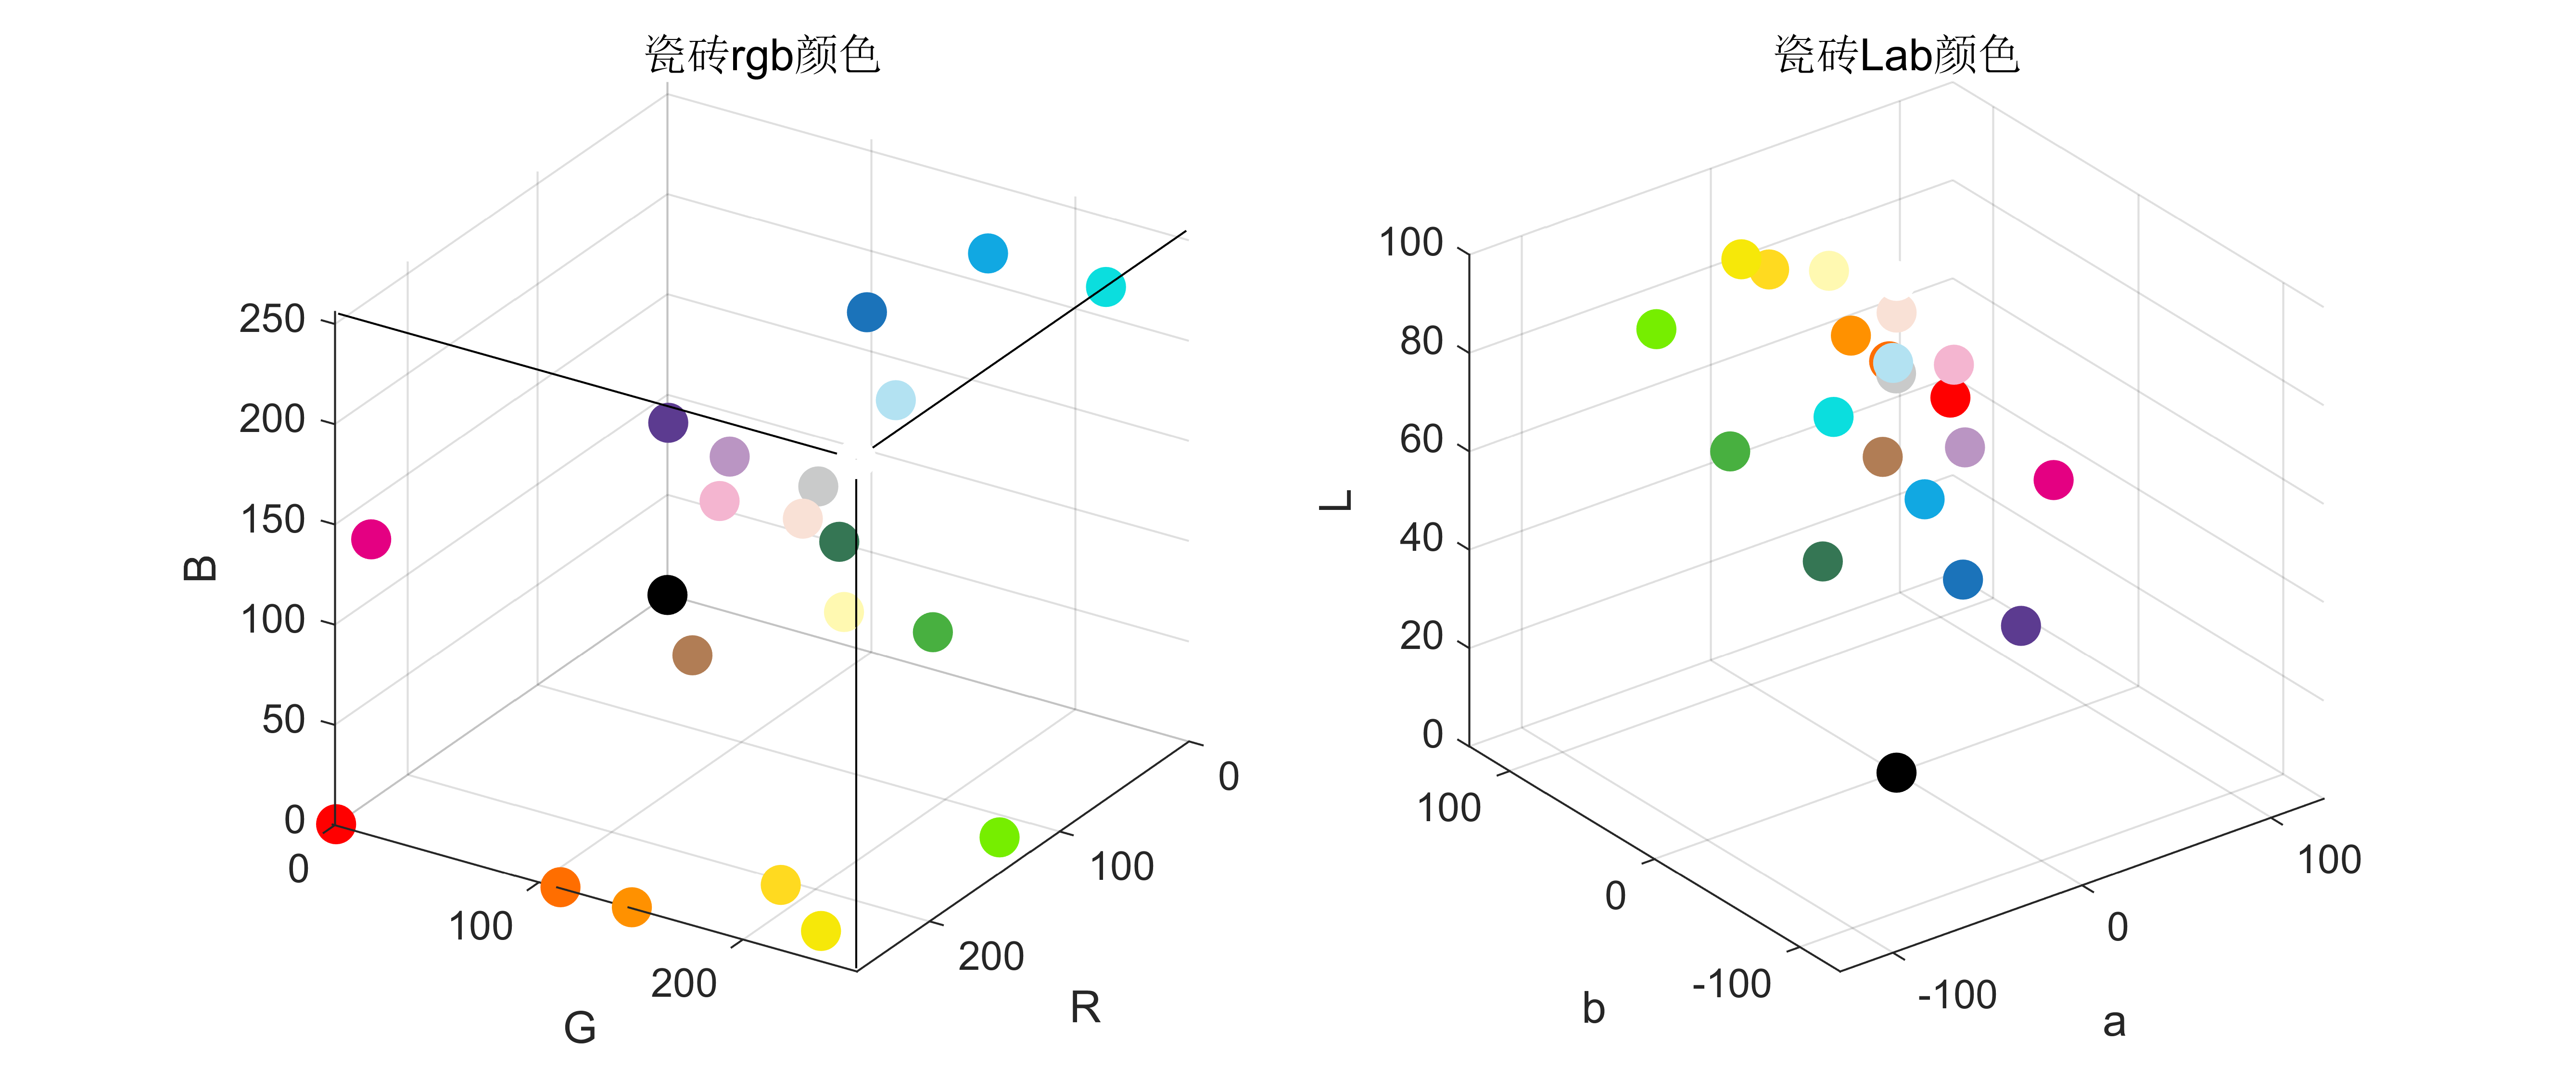
\includegraphics[width=0.85\textwidth]{img/瓷砖的rgb和Lab颜色.png}
 	\caption{瓷砖的rgb和Lab颜色}
 	\label{瓷砖的rgb和Lab颜色}
 \end{figure}
 \textbf{HSV颜色空间}:
 
 HSV是个六棱锥模型,这个模型中颜色的参数分别是:色调(H),饱和度(S),明度(V)。使用HSV空间计算距离时,存在一定的问题,比如,在接近顶点的地方,基本都接近黑色,不管H色调怎么改变,而在底面的中心或者S饱和度接近0时,基本都接近灰色,不管H色调怎么改变,而在饱和度S较大,且V亮度较大时,H色调的一点改变往往会让整体的颜色产生巨大变化,所以,用HSV计算距离时往往还存在某些问题.
 
  \textbf{LAB颜色空间}:
 
 LAB颜色空间是基于人眼对颜色的感知,可以表示人眼所能感受到的所有颜色。L表示明度,A表示红绿色差,B表示蓝黄色差。应用$\left(L_{1}^{*}, a_{1}^{*}, b_{1}^{*}\right)$和$\left(L_{2}^{*}, a_{2}^{*}, b_{2}^{*}\right)$两个L*a*b*色彩空间的颜色色差(CIE76公式\upcite{YanSeChaiYi2021}):
 \begin{equation}
 \Delta E_{a b}^{*}=\sqrt{\left(L_{2}^{*}-L_{1}^{*}\right)^{2}+\left(a_{2}^{*}-a_{1}^{*}\right)^{2}+\left(b_{2}^{*}-b_{1}^{*}\right)^{2}}
 \label{cie76}
 \end{equation}
 
 在1994年,人们将1976年的定义进行了进一步的发展,以更好地应对感知非均匀特性,提出CIE94公式。鉴于1994年的公式并没有充分解决感知非均匀特性的问题,CIE再次修缮了定义,形成了CIE2000公式\upcite{YanSeChaiYi2021}:
 \begin{equation}
 \Delta E_{00}^{*}=\sqrt{\left(\frac{\Delta L^{\prime}}{k_{L} S_{L}}\right)^{2}+\left(\frac{\Delta C^{\prime}}{k_{C} S_{C}}\right)^{2}+\left(\frac{\Delta H^{\prime}}{k_{H} S_{H}}\right)^{2}+R_{T} \frac{\Delta C^{\prime}}{k_{C} S_{C}} \frac{\Delta H^{\prime}}{k_{H} S_{H}}}
 \label{cie2000}
 \end{equation}
 
 为了简化计算及保证计算效果,有人在RGB空间上通过公式计算出加权的欧式距离\upcite{SeDuZhiBiao}(以下称简化公式)。其为加权欧氏距离函数的组合,权重因子取决于颜色的“红色”分量有多大。首先计算“红色”的平均水平,然后加权$\Delta R^{\prime}$ 和 $\Delta B^{\prime}$信号作为平均红色水平的函数。颜色$C_1$和$C_2$之间的距离(红色,绿色和蓝色通道中的每个通道的范围为0-255):
 \begin{equation}
 \begin{array}{l}
 \bar{r}=\frac{C_{1, R}+C_{2, R}}{2} \\
 \Delta R=C_{1, R}-C_{2, R} \\
 \Delta G=C_{1, G}-C_{2, G} \\
 \Delta B=C_{1, B}-C_{2, B} \\
 \Delta E=\sqrt{\left(2+\frac{\bar{r}}{256}\right) \times \Delta R^{2}+4 \times \Delta G^{2}+\left(2+\frac{255-\bar{r}}{256}\right) \times \Delta B^{2}}
 \end{array}
 \label{jianhuags}
 \end{equation}
 
 经过测试,CIEDE2000色差公式与简化公式计算方法的效果对比,结果各有千秋,具体使用哪种方法,看应用场景测试决定。
 \subsection{空间点集均匀性的计算}
 \subsubsection{独占线,独占圆,独占球,和独占体的定义}
 独占线,独占圆,独占球,和独占体的定义\upcite{luoDianKongJianFenXiFenWeiYuJunYunDu2004}:
 
 独占线:在一维欧氏空间中的一个闭区间内分布的点集,对于左右都有邻体的点b,设ab 线段与bc 线段长度的最小者为s,则以b点为中心,以s/2为半径的区间为b点的独占线;
  \begin{figure}[H]
 	\centering
 	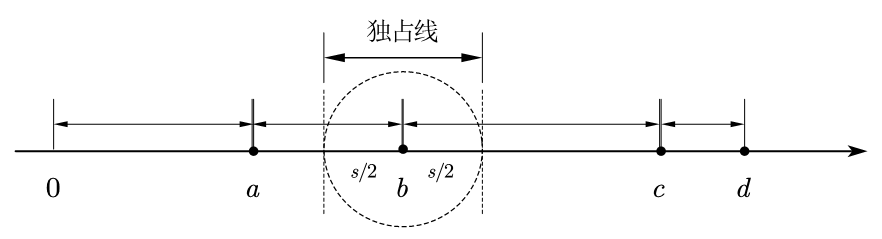
\includegraphics[width=0.85\textwidth]{img/独占线.png}
 	\caption{独占线}
 	\label{独占线}
 \end{figure}

 同理,可定义独占圆,独占球,和独占体:
 
 独占圆:在2维欧氏空间中,对于一定空间范围内分布的点集,设任意一点与最近邻体的距离为s,以s/2为半径所
 画的圆为该点的独占圆;
   \begin{figure}[H]
 	\centering
 	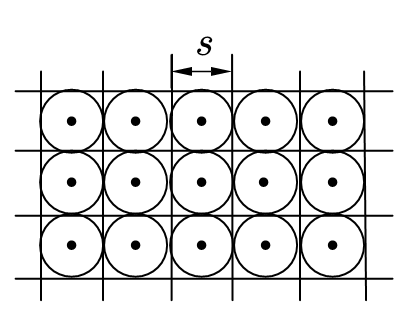
\includegraphics[width=0.45\textwidth]{img/独占圆.png}
 	\caption{独占圆}
 	\label{独占圆}
 \end{figure}
 独占球:考虑在n 维欧氏空间中的点集,设任意一点与最近邻体的距离为s,则称以该点为球心$s/2$ 为半径所画的球为该点的独占球。
 
 独占体:一个独占圆的外接正方形称之为独占方,一个n维球的外接n维正方体称之为n维独占体.
 
 \subsubsection{点集均匀性的计算}
 在1维欧氏空间中区间$[a,b]$上的点集,点集的独占线总长度与区间长度之比称为1 维点集的均匀度若独占线长度正好等于区间长度, 则称之为1维完全均匀分布\upcite{shenErWeiLiZiFenBuJunYunDuCeSuanFangFaYanJiu1993}。设均匀度为$J$,由于区间的总长度是固定的(对于2维,面积固定;对于3维,体积固定,因此只需要计算分子的大小)则易知一维点集均匀度与独占线的和成正比,即:
 \begin{equation}
 J \propto \sum_{i=1}^{n} s_{i}\,\, ,n\text{为点的数量}
 \end{equation}
 同理,对于n维点集,
 \begin{equation}
 J\propto \sum_{i=1}^n{s}_{i}^{n}\,\, ,n\text{为点的数量}
 \end{equation}
 所以评价颜色在3维颜色空间(Lab)中的均匀度可以使用以下公式:
 \begin{equation}
 J \propto  \sum_{i=1}^{n} s_{i}^{3}\,\, ,n\text{为点的数量}
 \label{j3}
 \end{equation}
 
 \section{问题一的求解}
 作出两张图片颜色的LAB空间分布如图\ref{txlab},
    \begin{figure}[H]
 	\centering
 	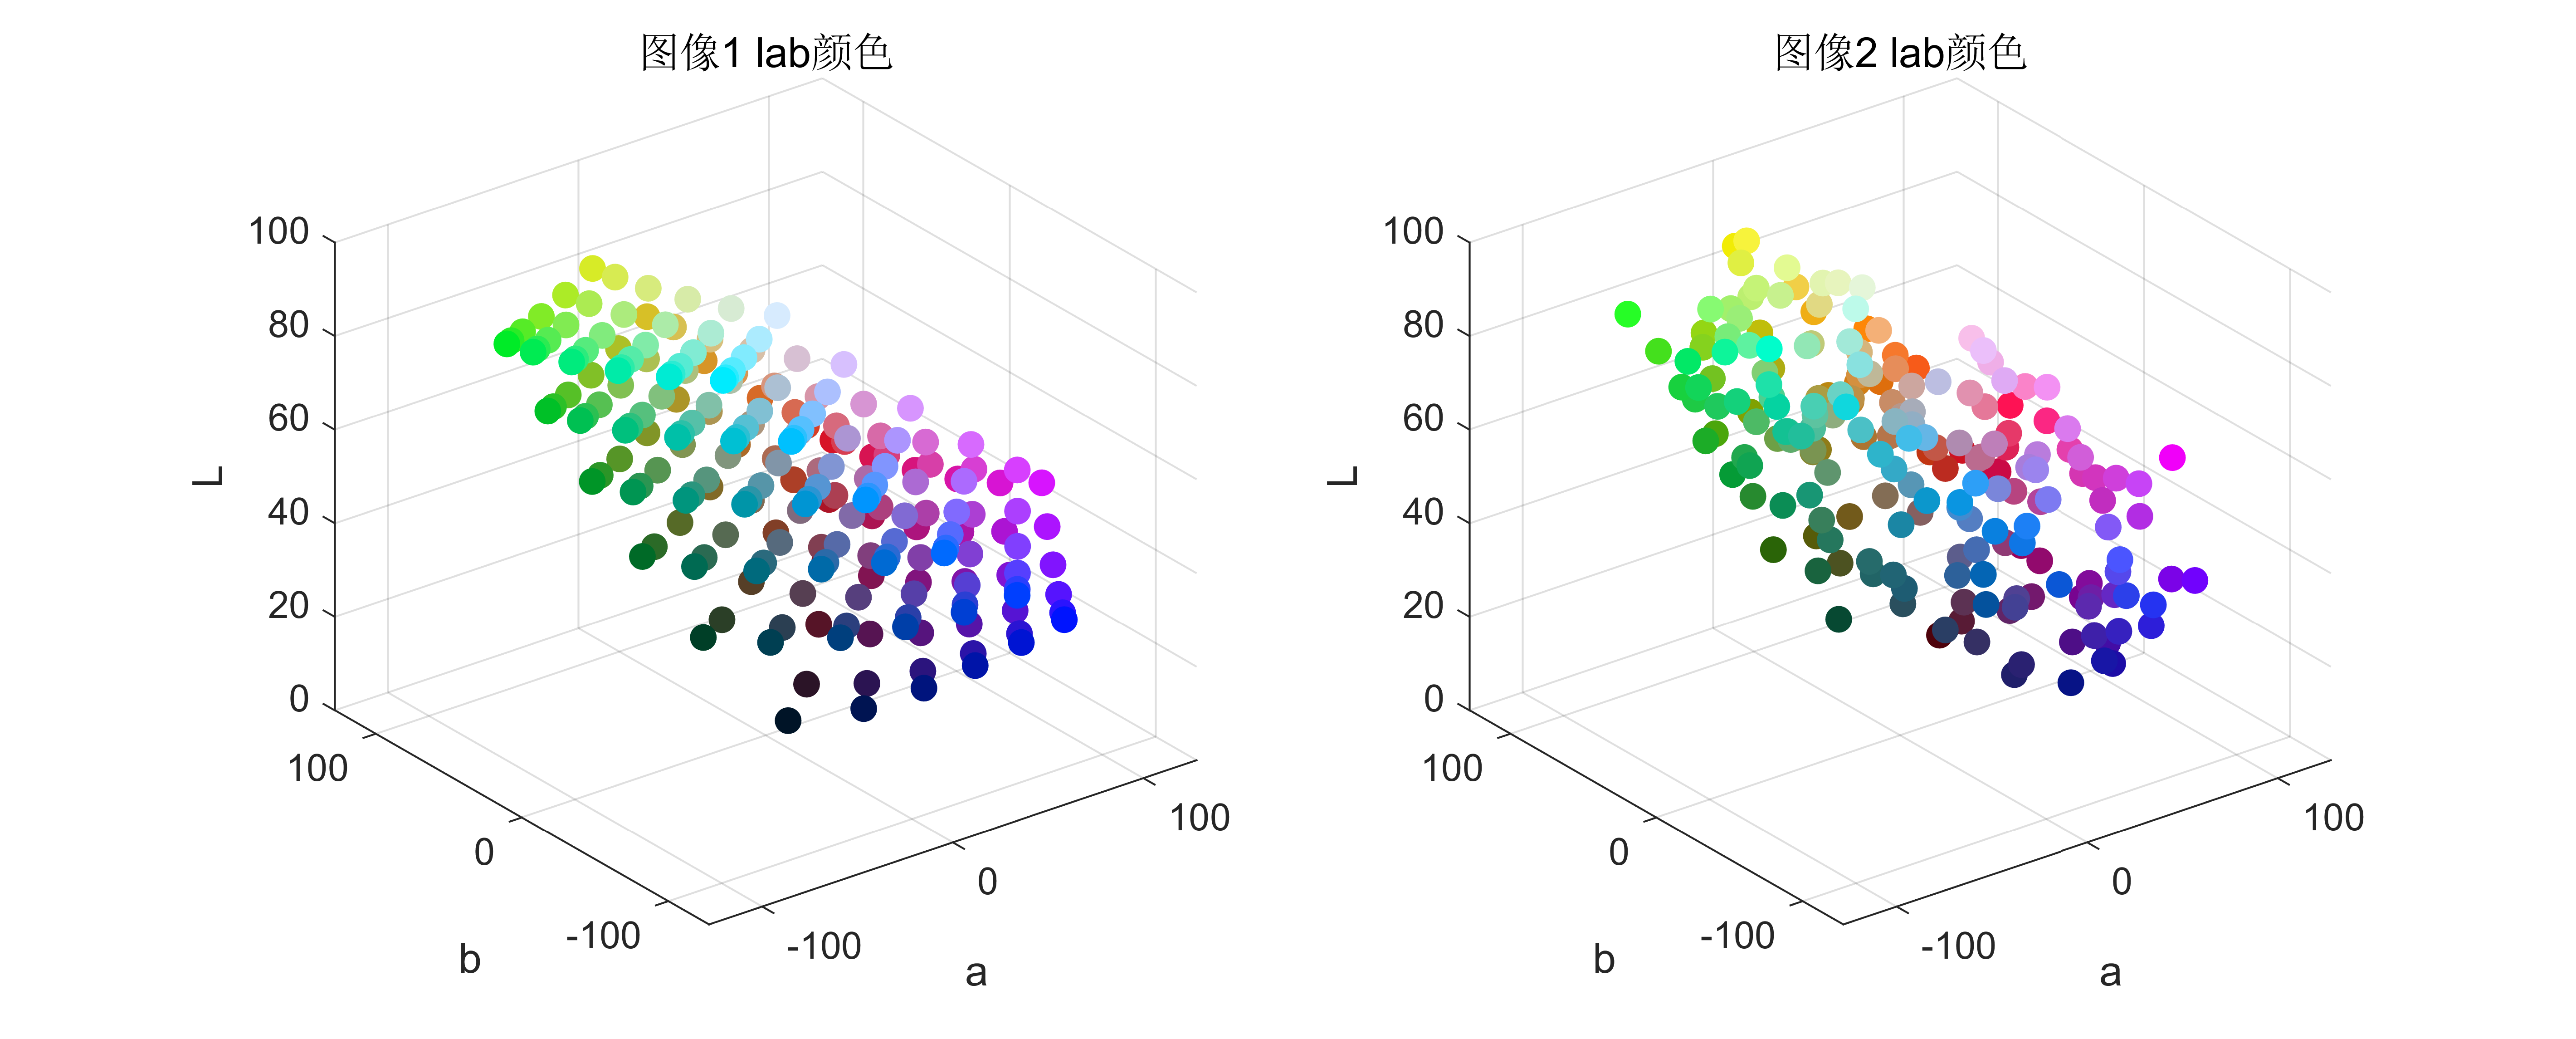
\includegraphics[width=0.9\textwidth]{img/图像12的lab颜色.png}
 	\caption{图像1 2的lab颜色}
 	\label{txlab}
 \end{figure}
 找出两张图片每种颜色最接近的瓷砖颜色,就是求每种颜色与22种瓷砖颜色的距离$\Delta E$,$\Delta E$越大,相似度越小,所以需要找到最小的$\Delta E$对应的瓷砖颜色。本问题的求解使用两种算法(CIE76 公式\eqref{cie76}和CIE2000 公式\eqref{cie2000})分别计算。
 算法的流程图如下:
   \begin{figure}[H]
 	\centering
 	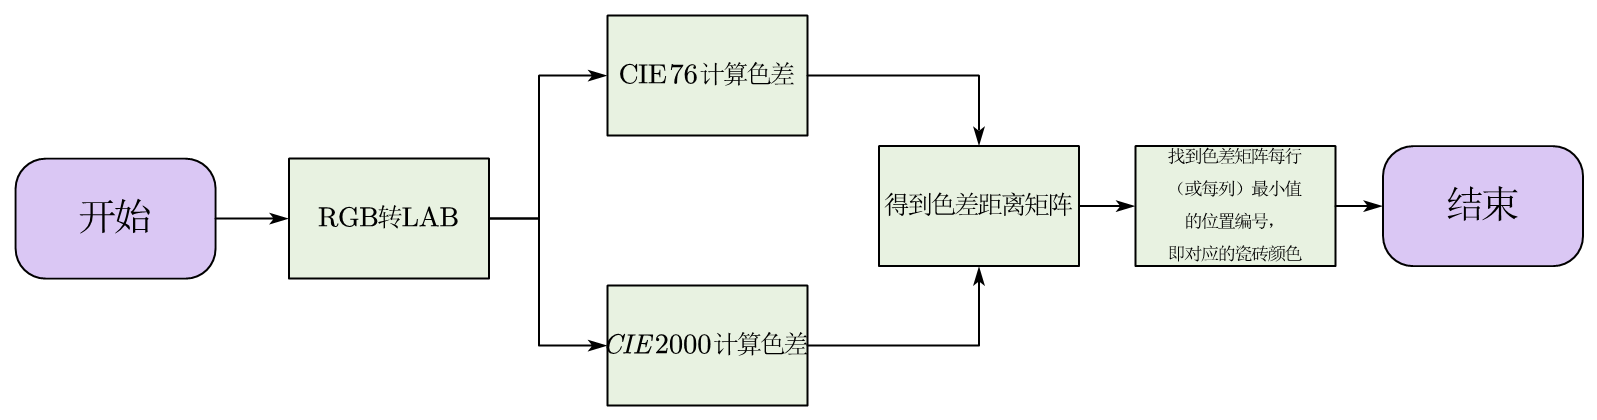
\includegraphics[width=0.85\textwidth]{img/问题1流程图.png}
 	\caption{问题1流程图}
 	\label{问题1流程图}
 \end{figure}
计算结果见附录。
其中使用CIE2000计算的结果绘制成网络连接图如下,图中大点为瓷砖颜色点,小点为图像颜色点。从拓扑图分析,算法的匹配效果很好。
	 \begin{figure}[H]
	\centering
	\subfigure[图像1的RGB网络连接]{
		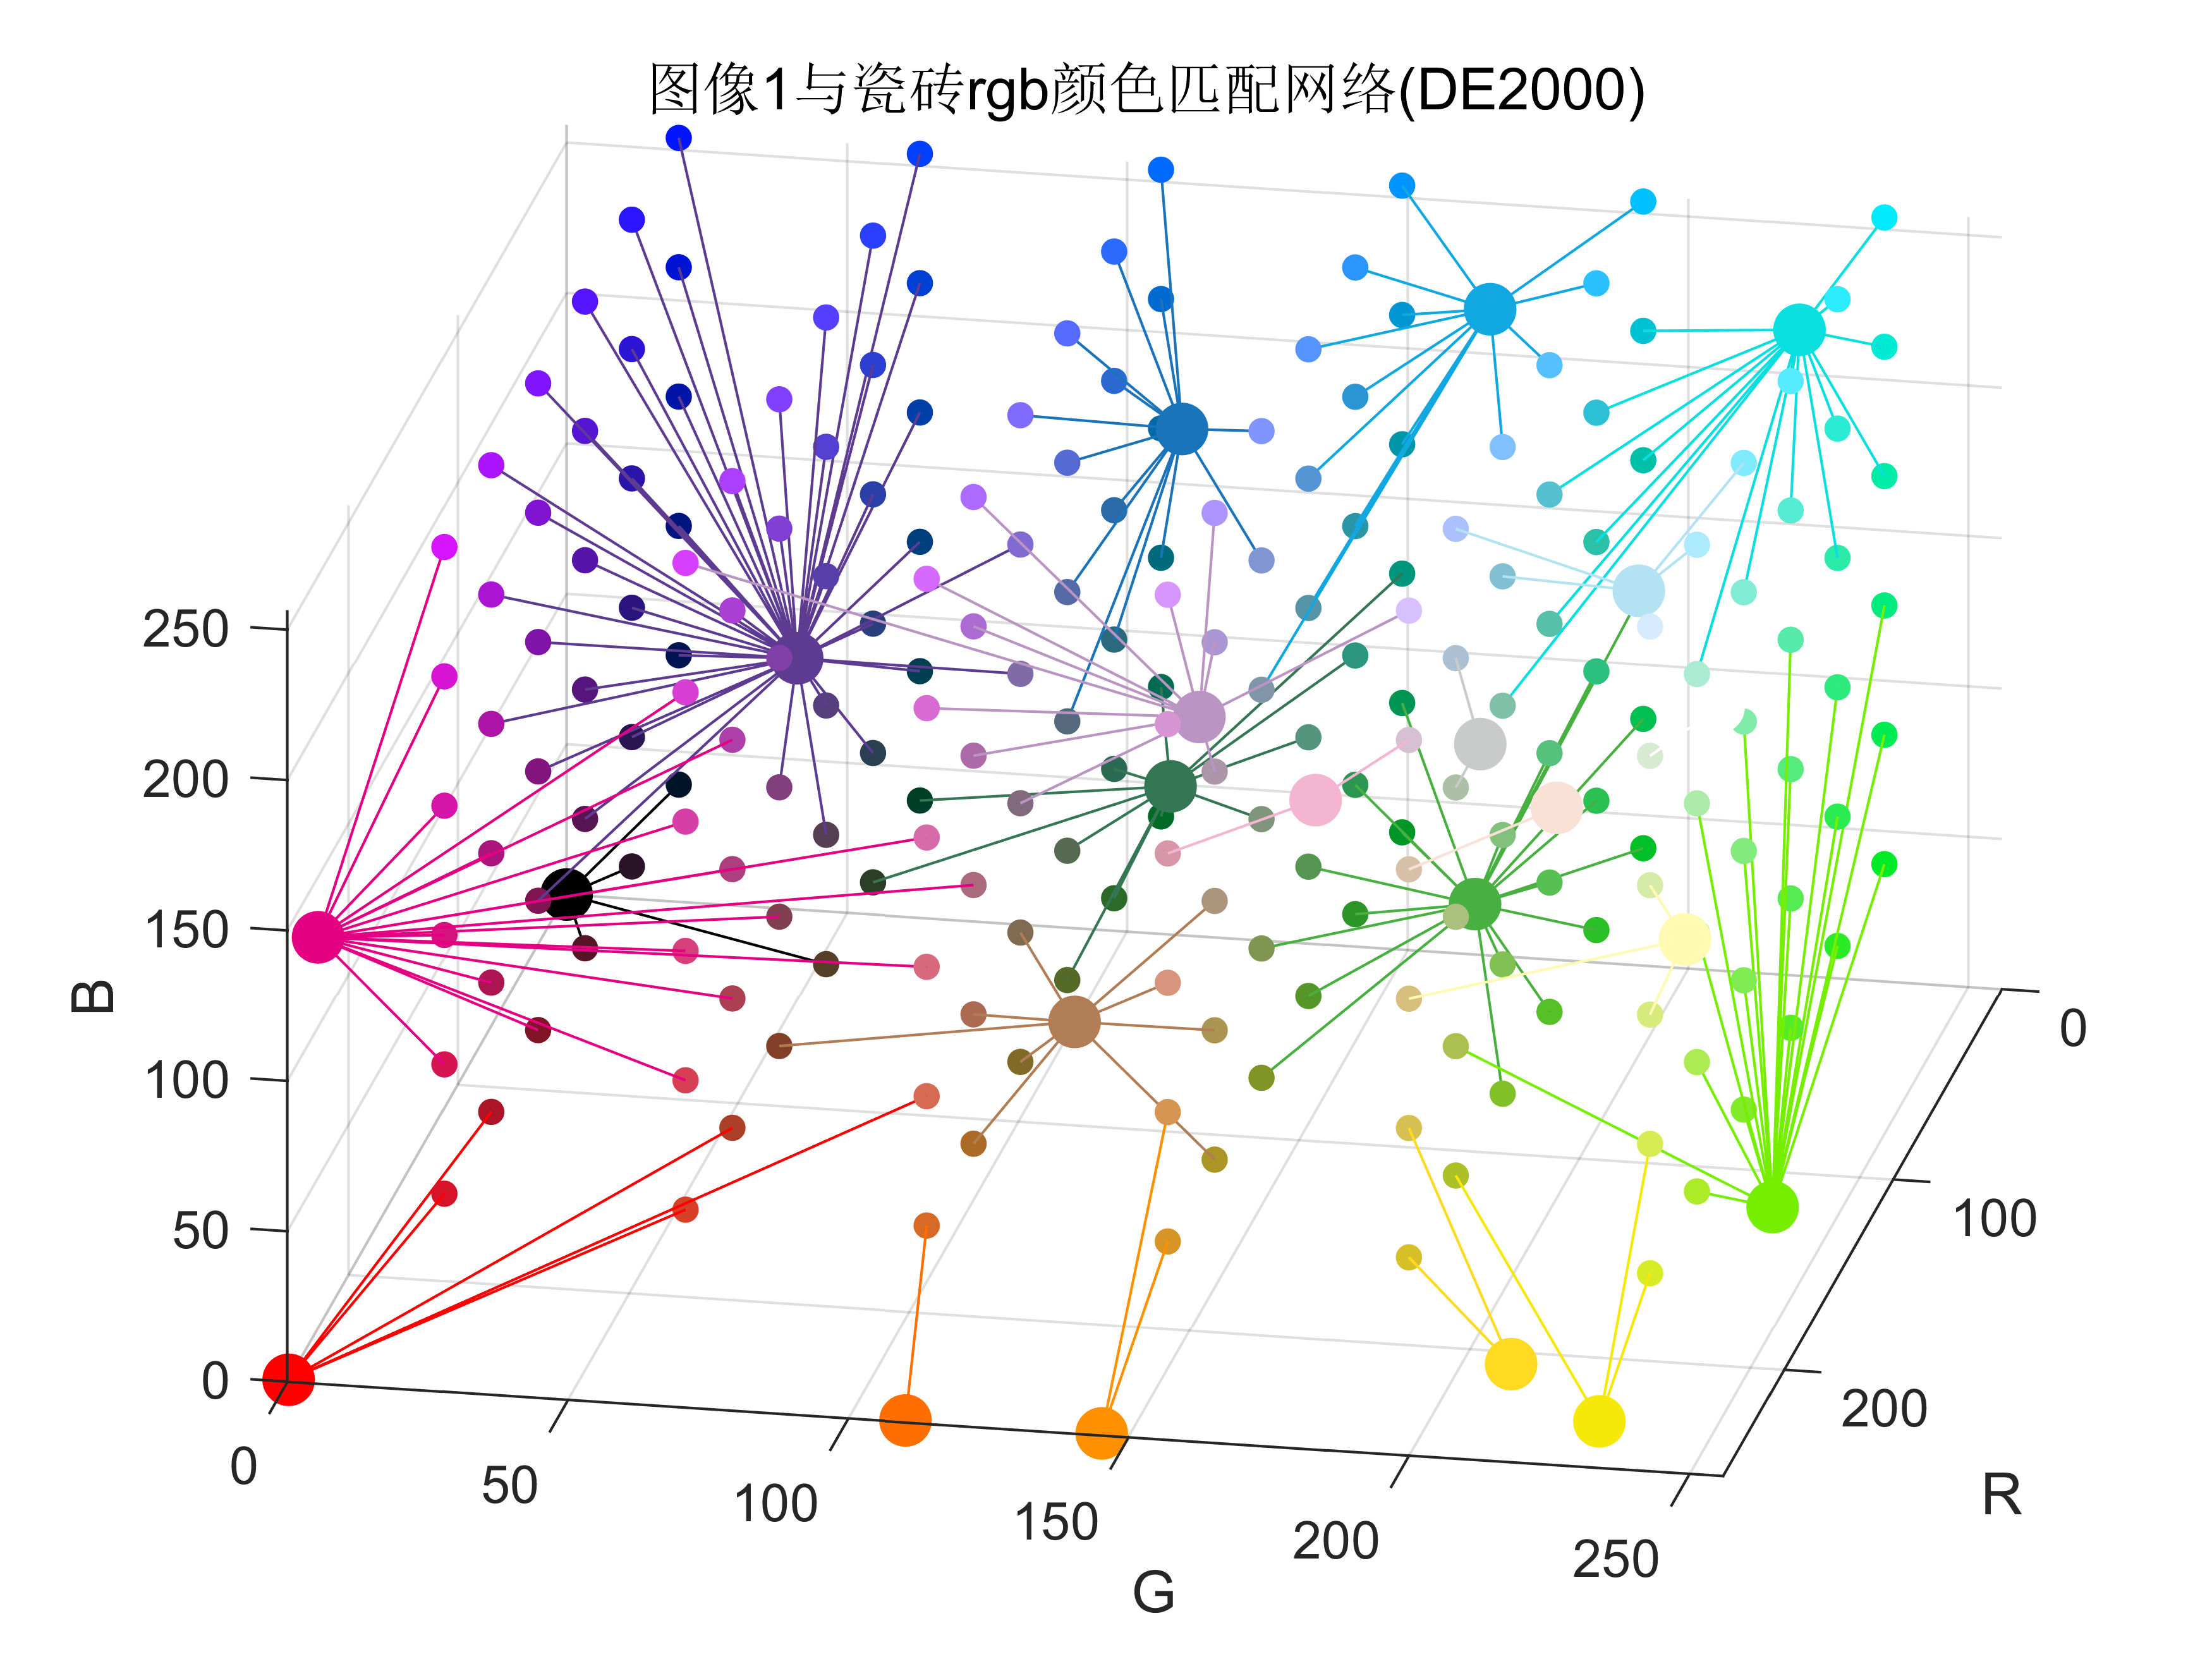
\includegraphics[width=0.47\linewidth]{img/图像1与瓷砖rgb颜色匹配网络DE2000.png}
		%\caption{fig1}
	}
	\quad
	\subfigure[图像2的RGB网络连接]{
		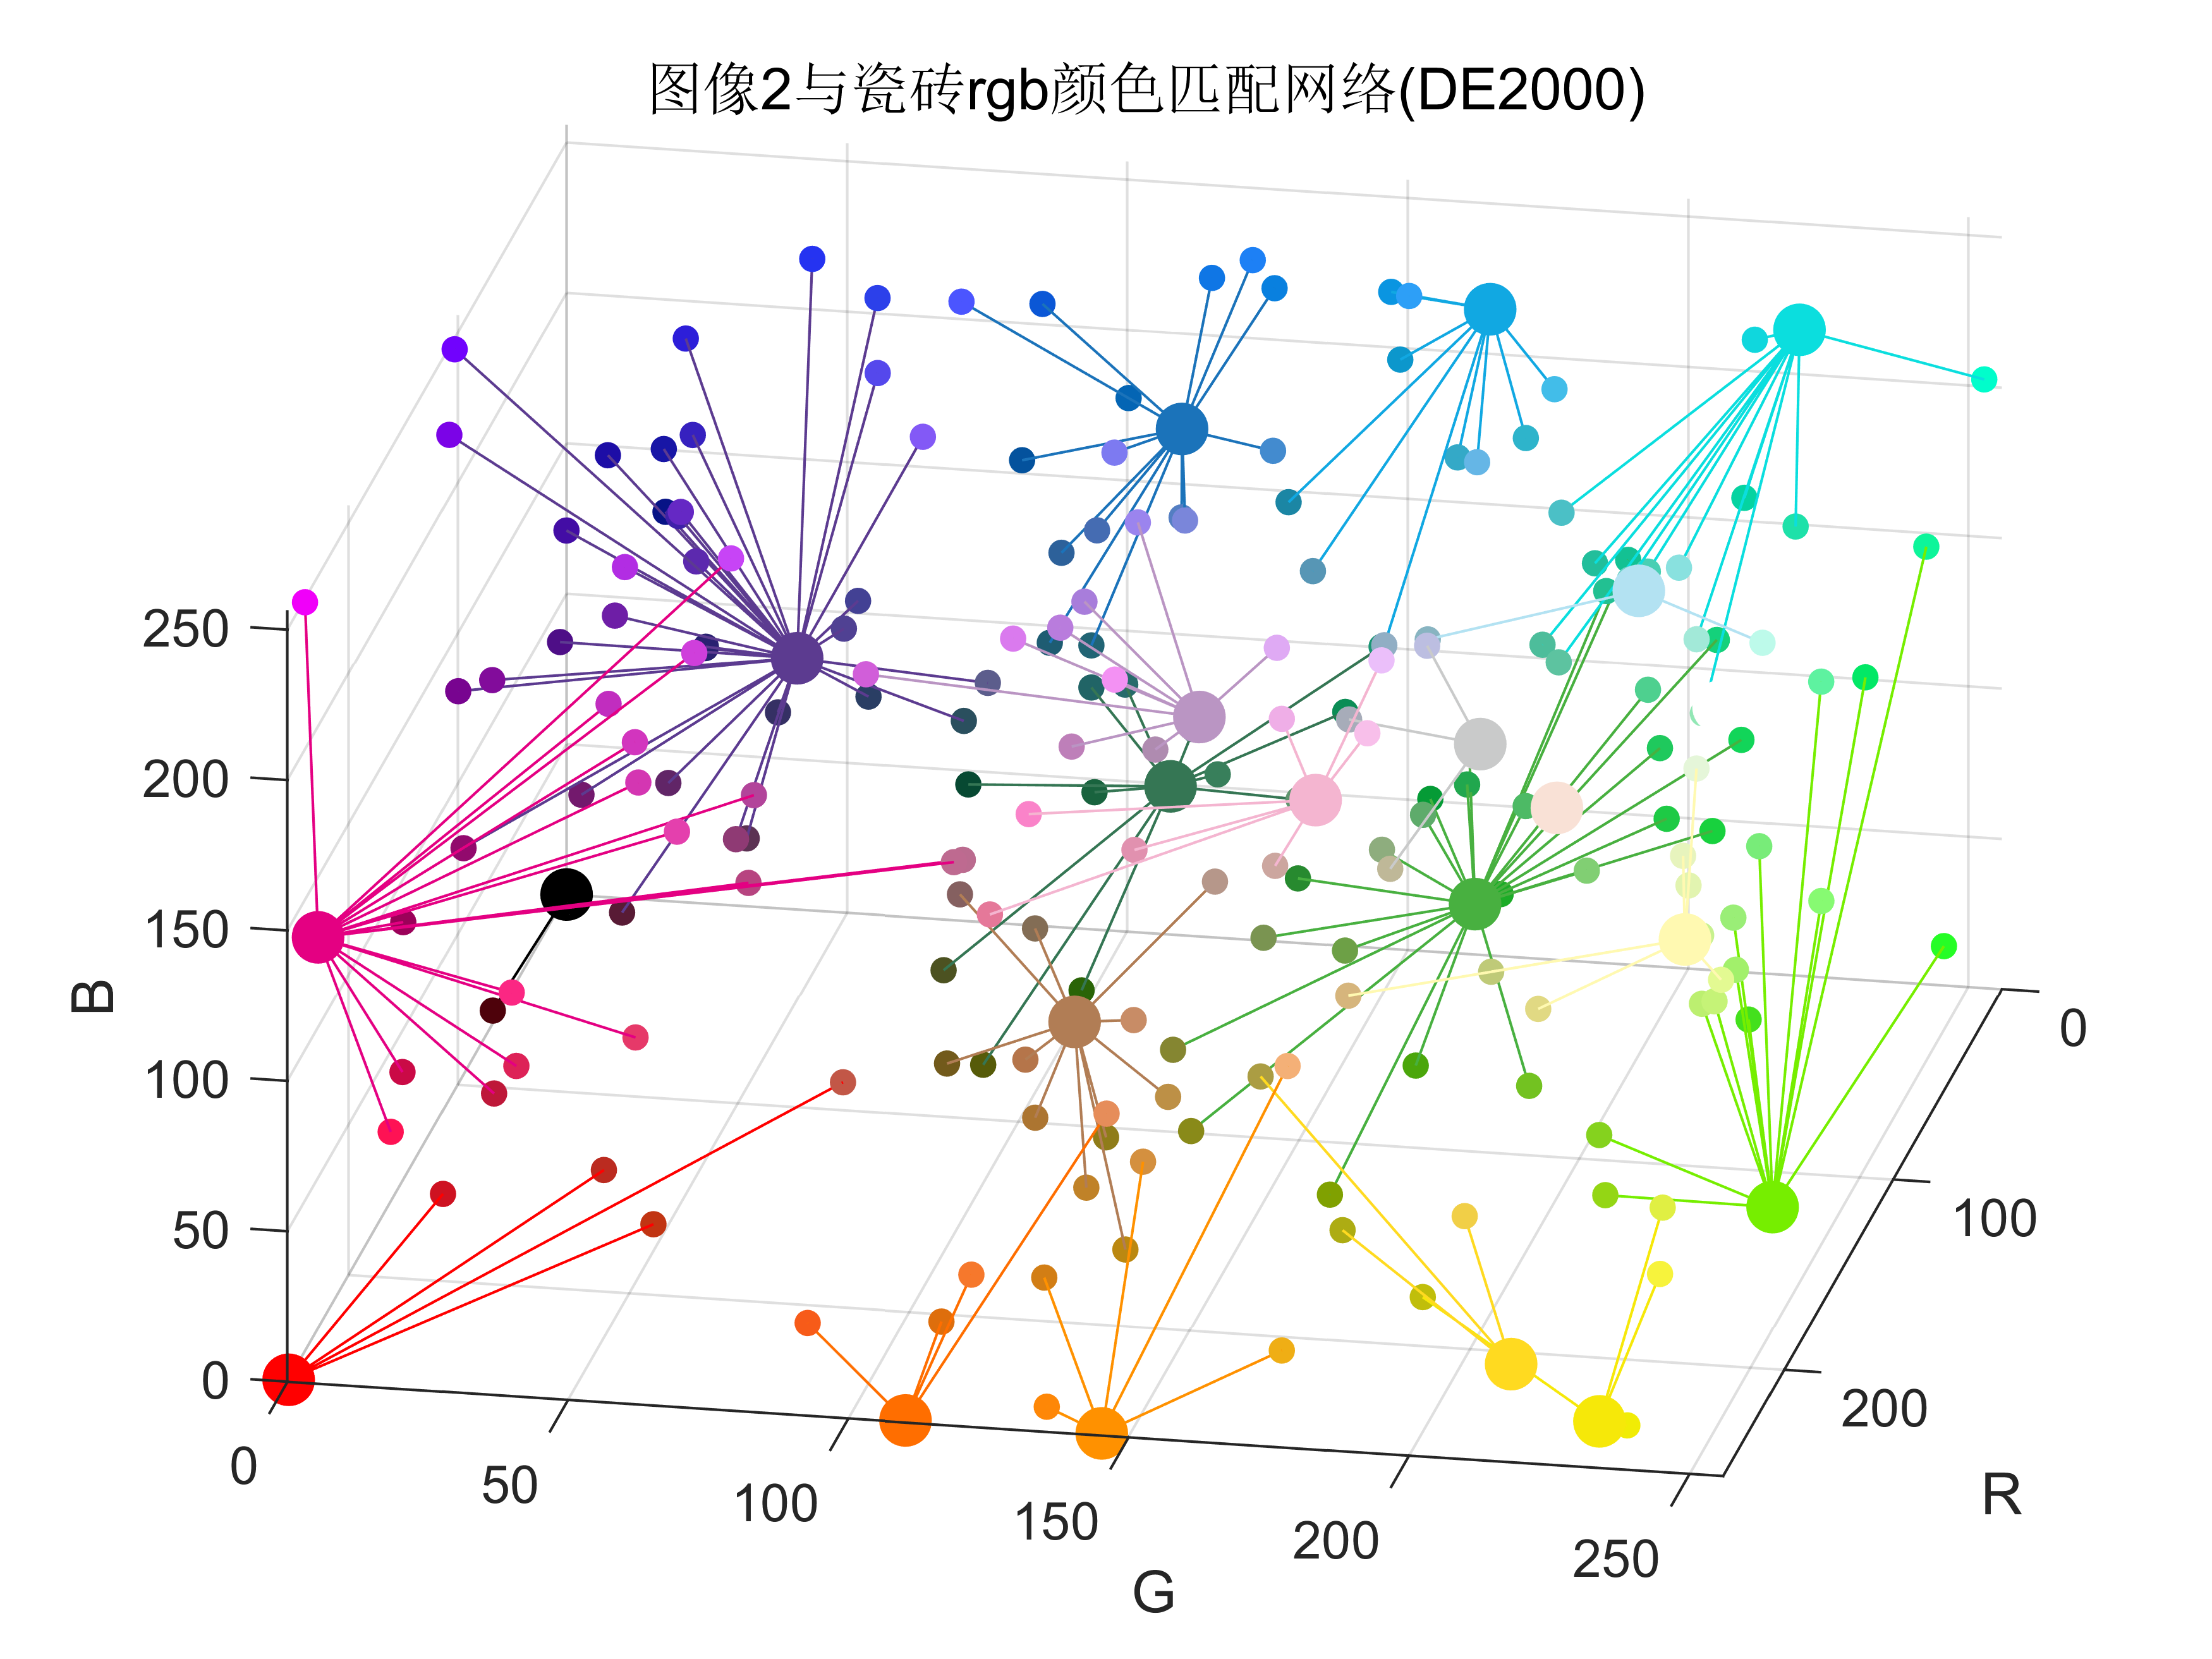
\includegraphics[width=0.47\linewidth]{img/图像2与瓷砖rgb颜色匹配网络DE2000.png}
	}
	\caption{图像1,2在RGB空间中的网络连接拓扑图(CIE2000)}
	\label{fig:rgbcie2000}
\end{figure}
	 \begin{figure}[H]
	\centering
	\subfigure[图像1的RGB网络连接]{
		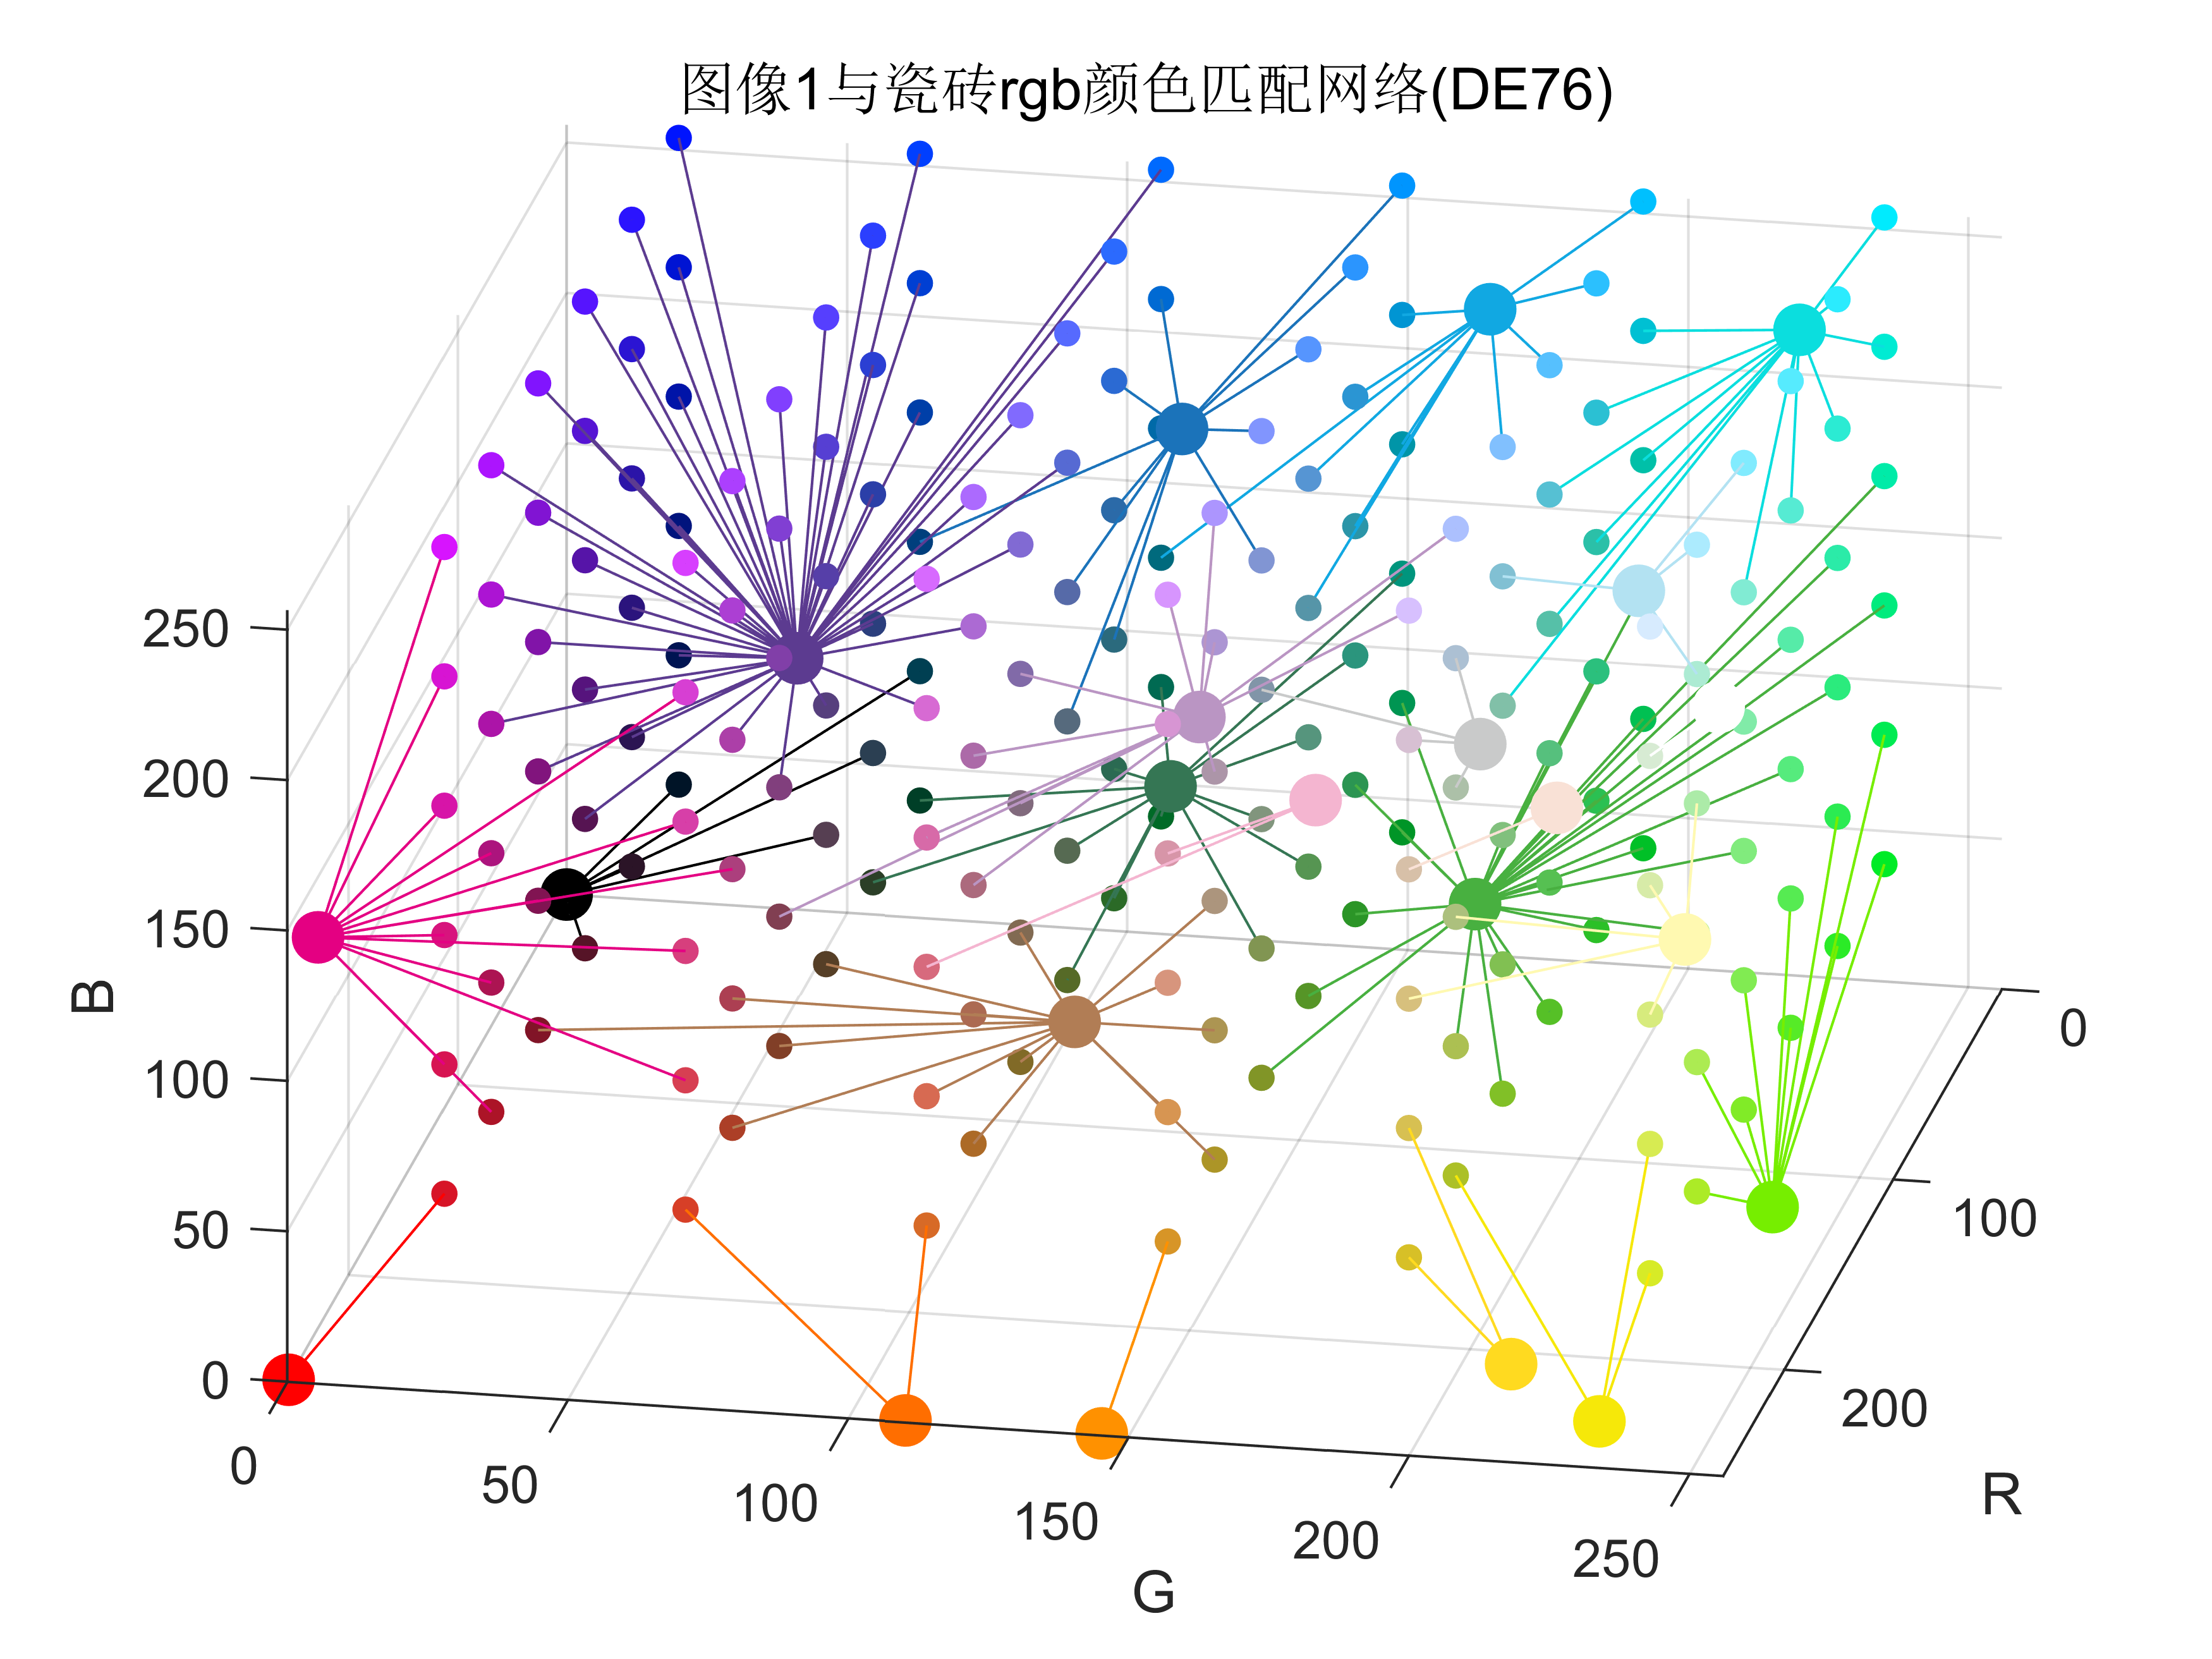
\includegraphics[width=0.47\linewidth]{img/图像1与瓷砖rgb颜色匹配网络DE76.png}
		%\caption{fig1}
	}
	\quad
	\subfigure[图像2的RGB网络连接]{
		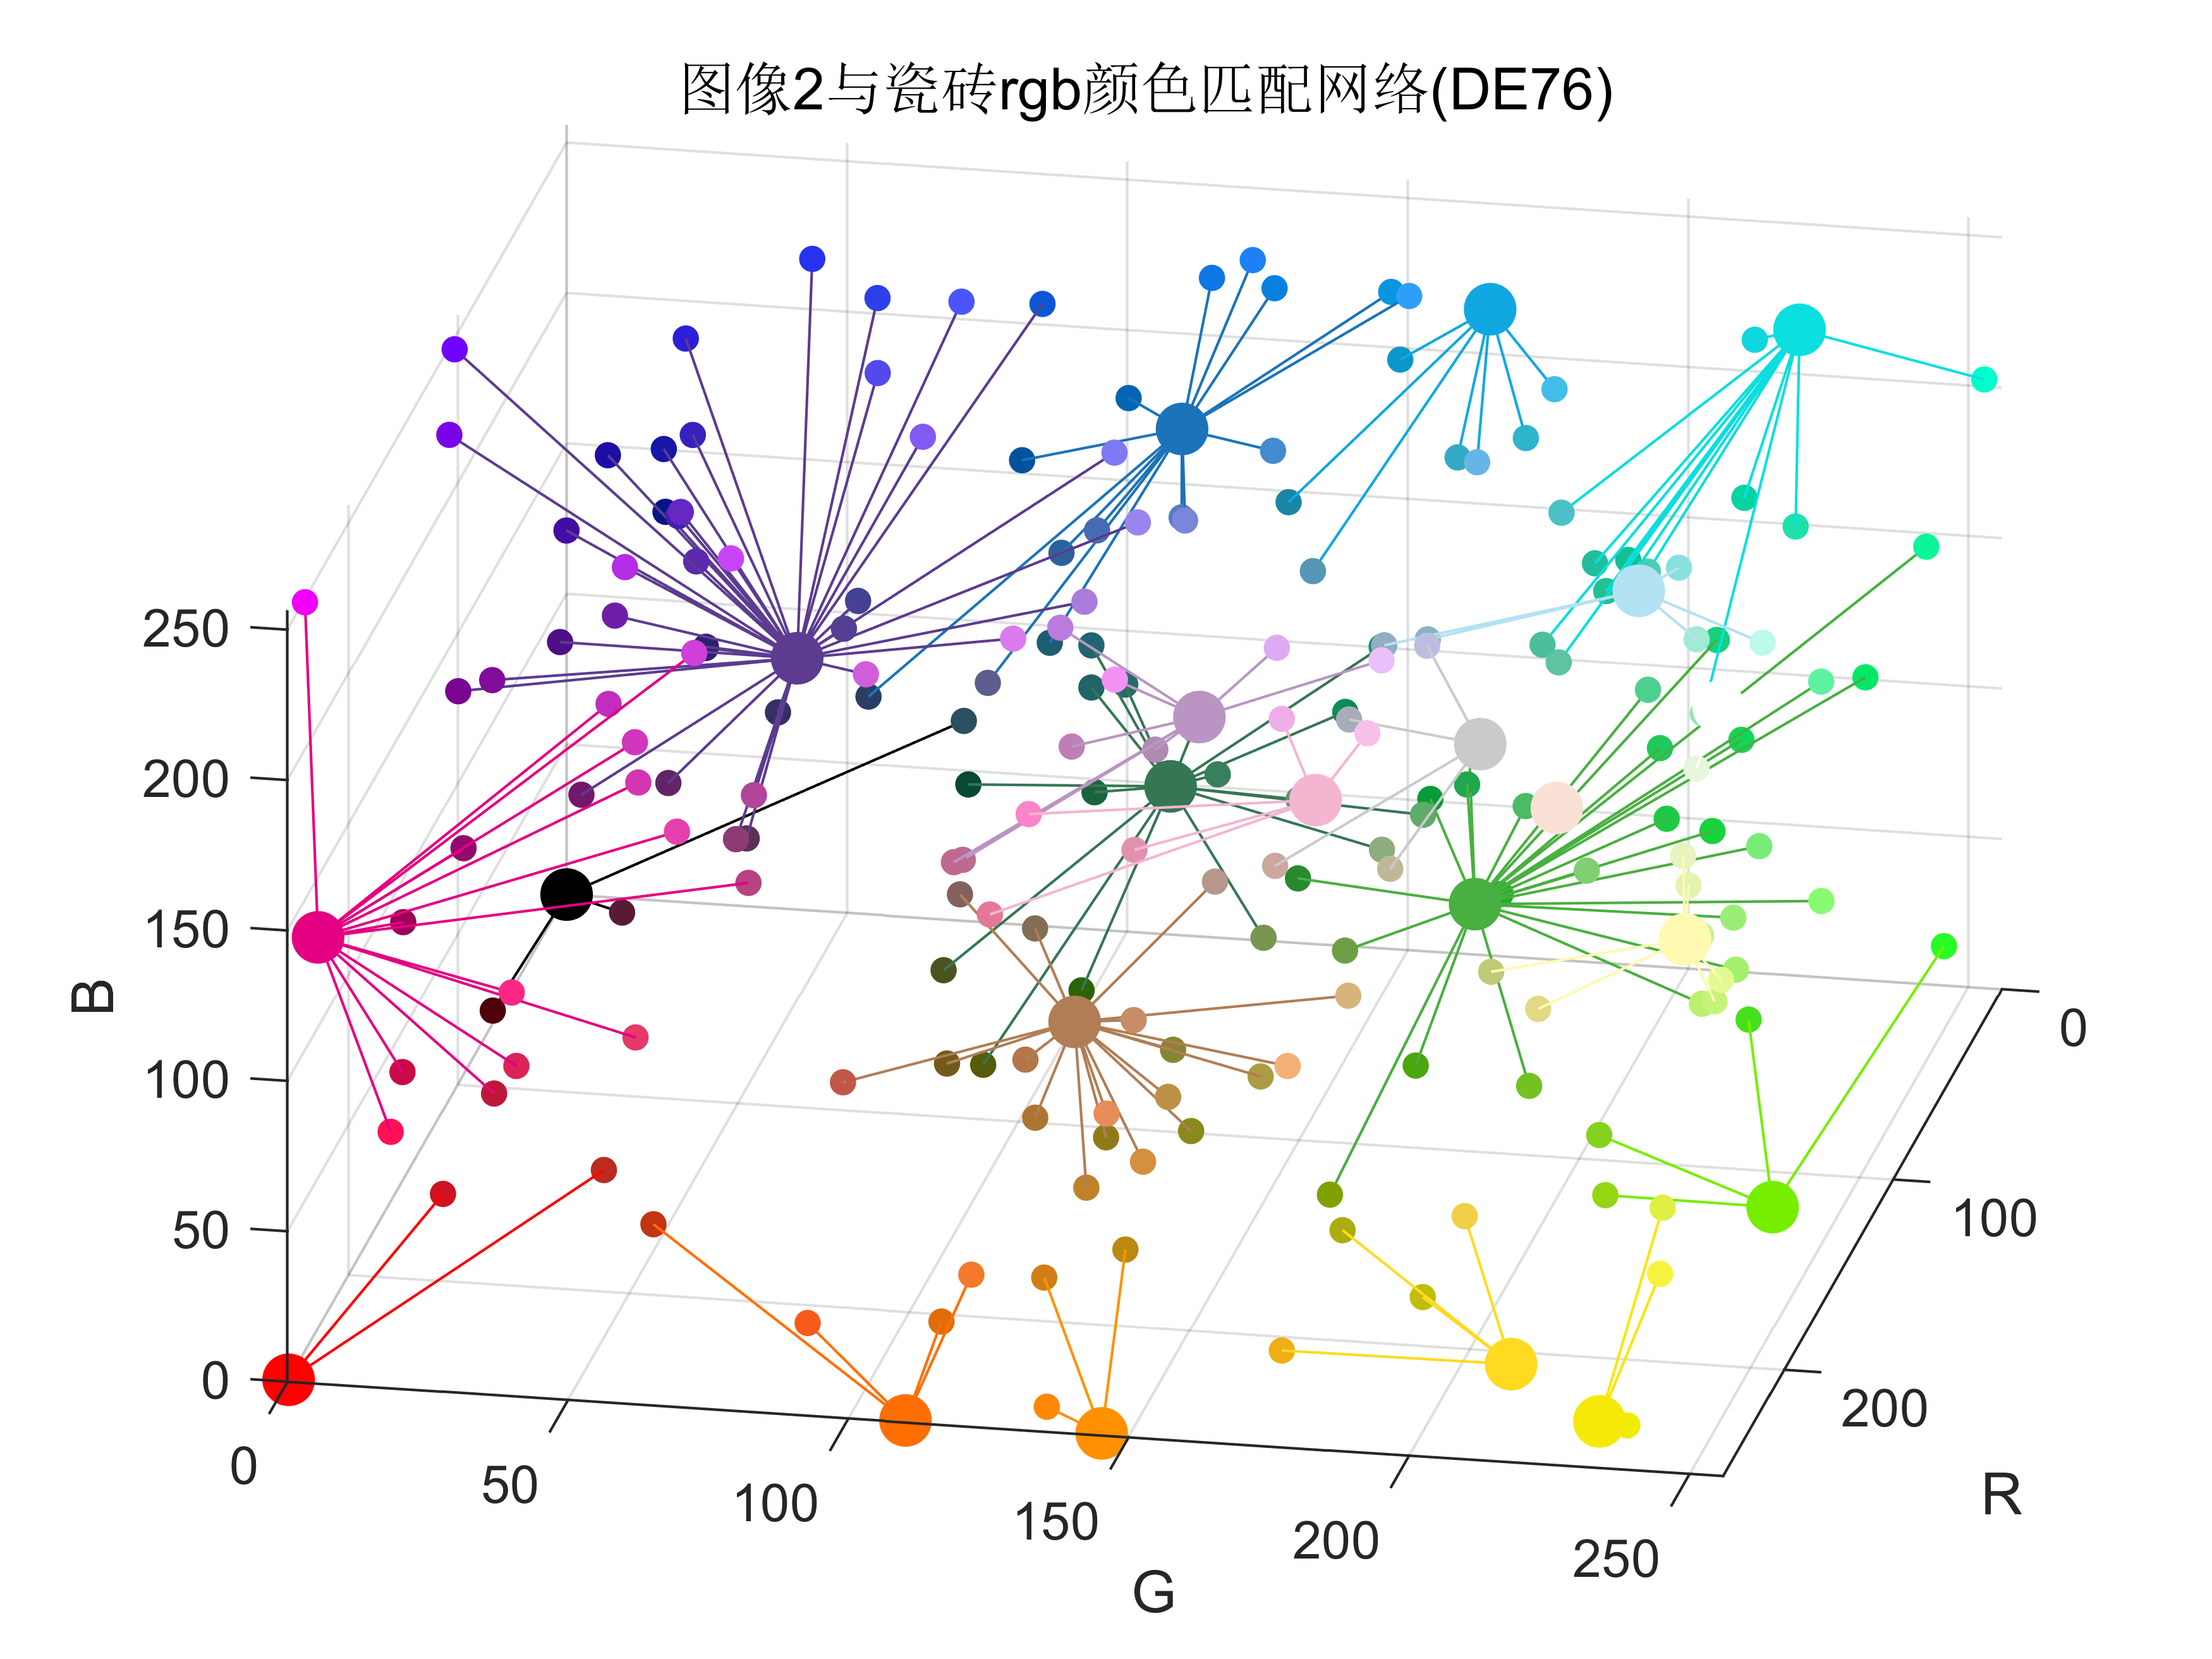
\includegraphics[width=0.47\linewidth]{img/图像2与瓷砖rgb颜色匹配网络DE76.png}
	}
	\caption{图像1,2在RGB空间中的网络连接拓扑图(CIE76)}
	\label{fig:rgbcie76}
\end{figure}
	 \begin{figure}[H]
	\centering
	\subfigure[图像1的LAB网络连接]{
		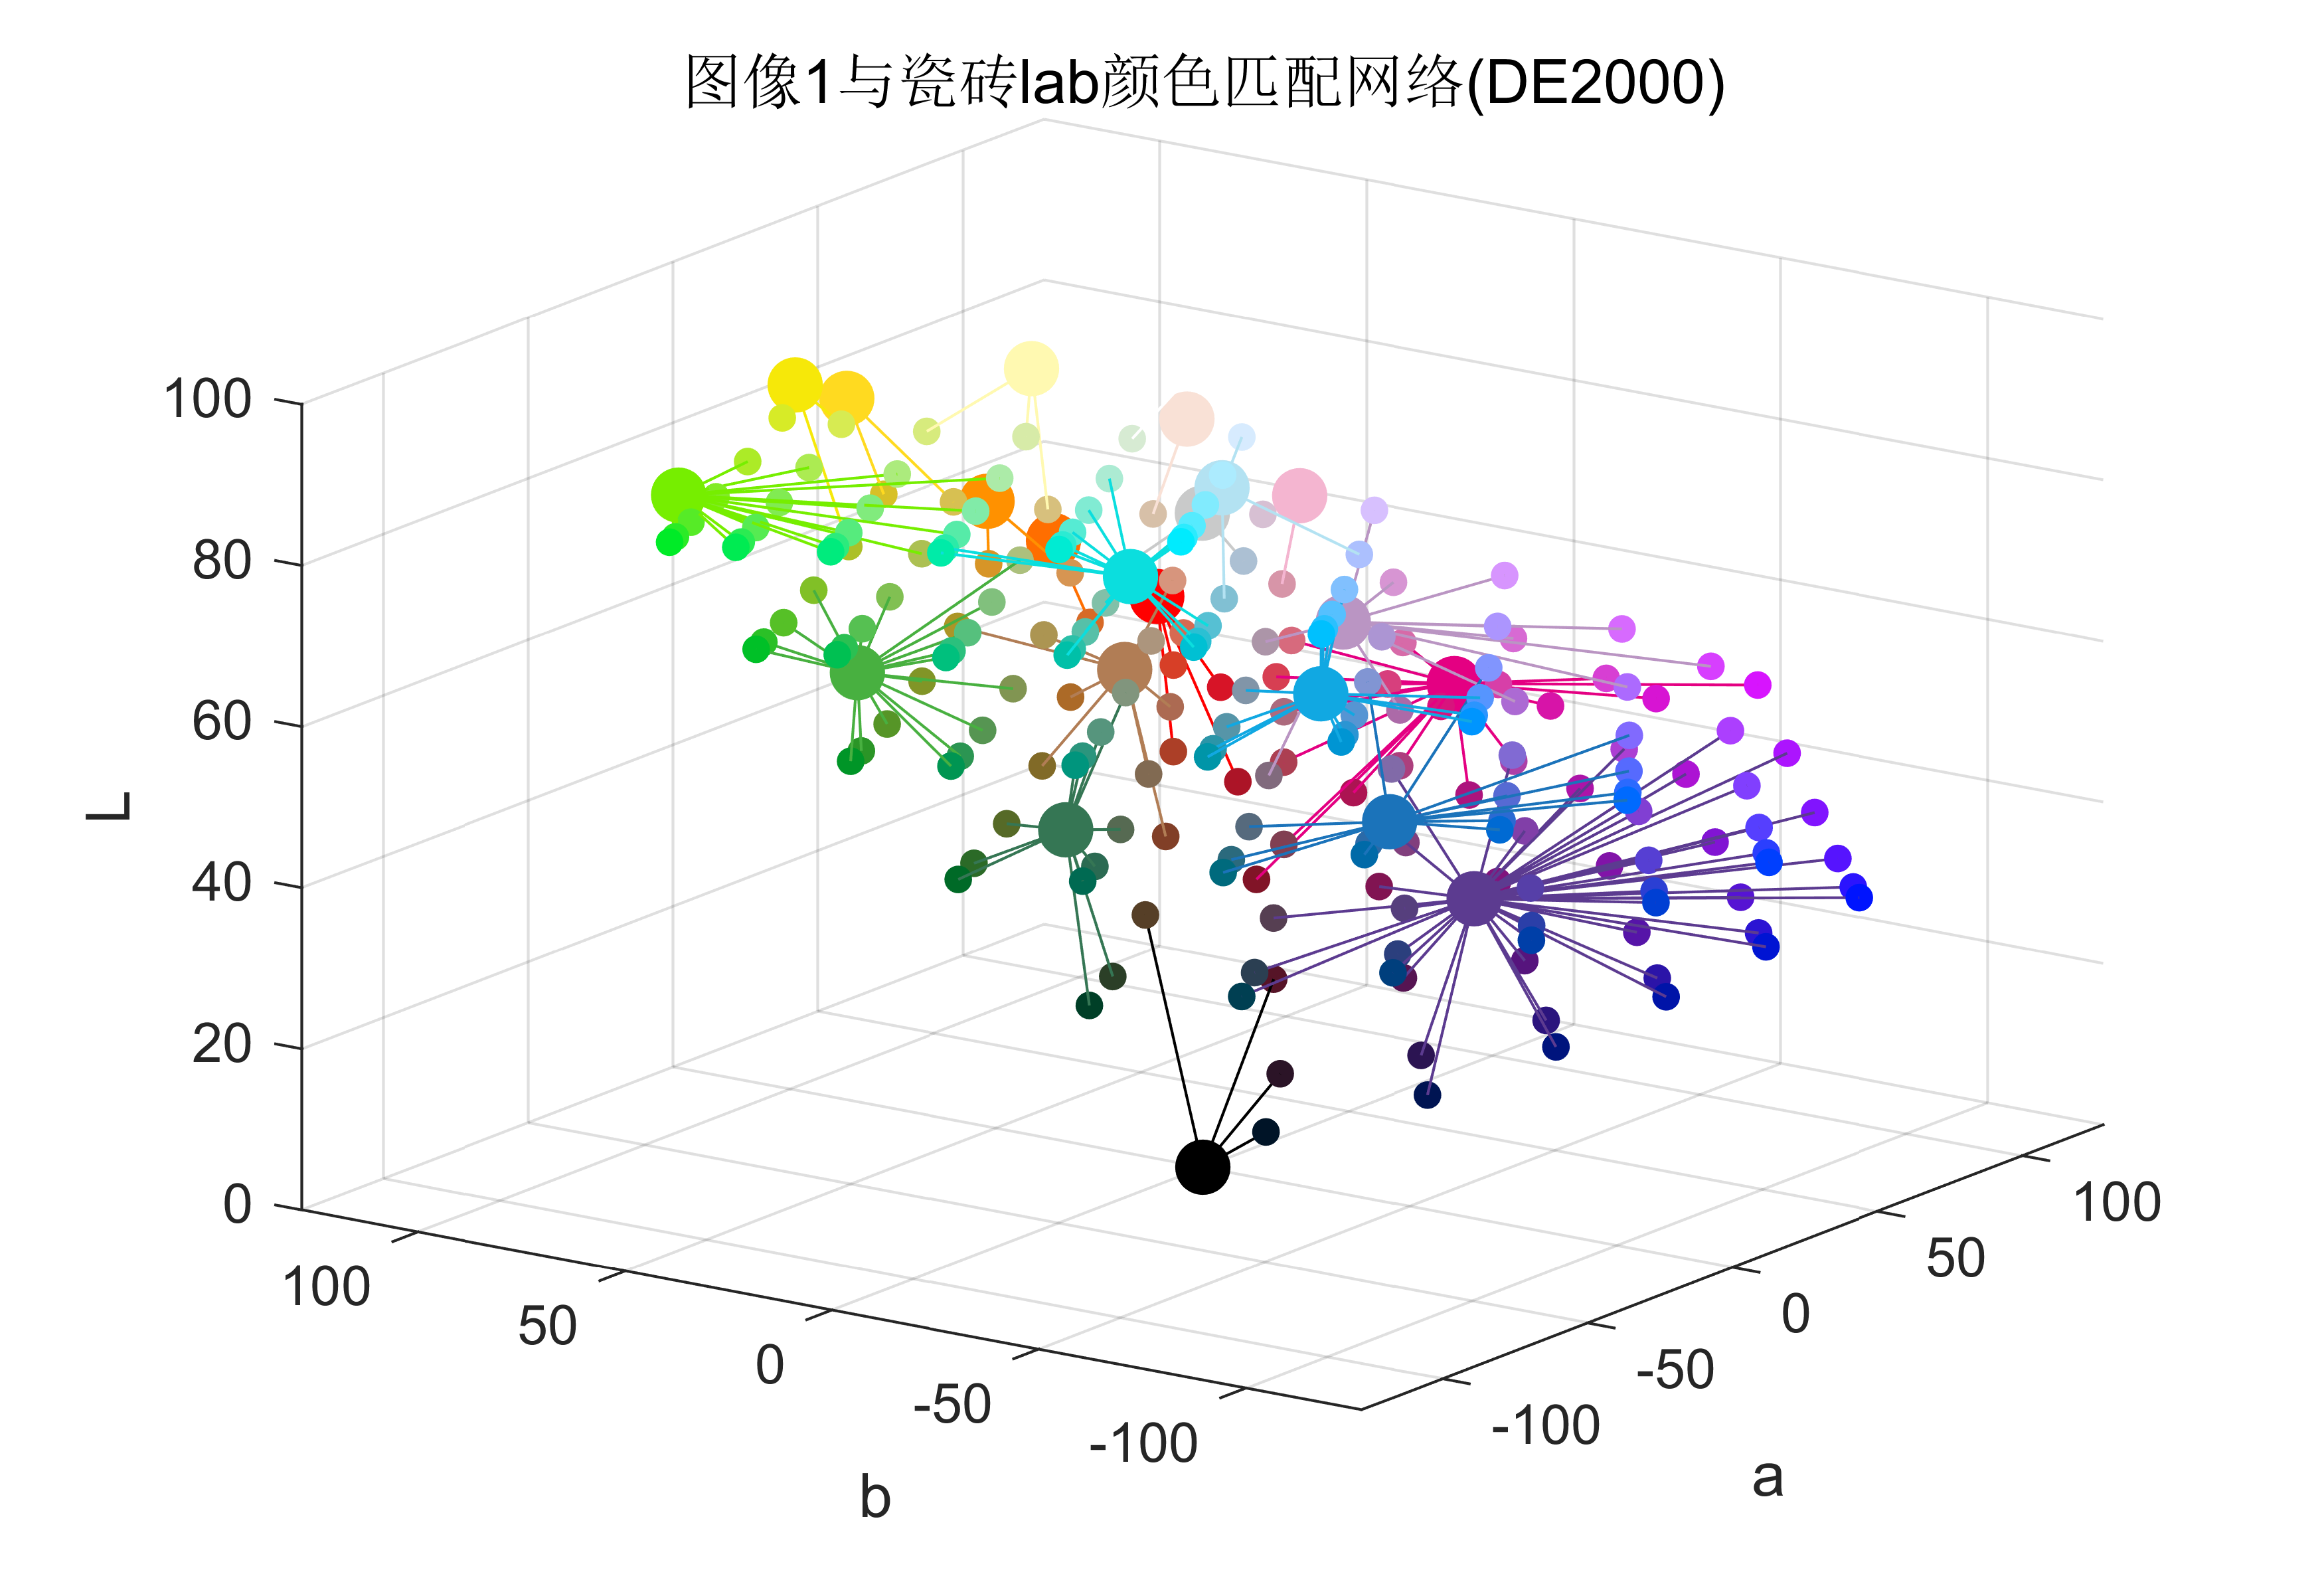
\includegraphics[width=0.47\linewidth]{img/图像1与瓷砖lab颜色匹配网络DE2000.png}
		%\caption{fig1}
	}
	\quad
	\subfigure[图像2的LAB网络连接]{
		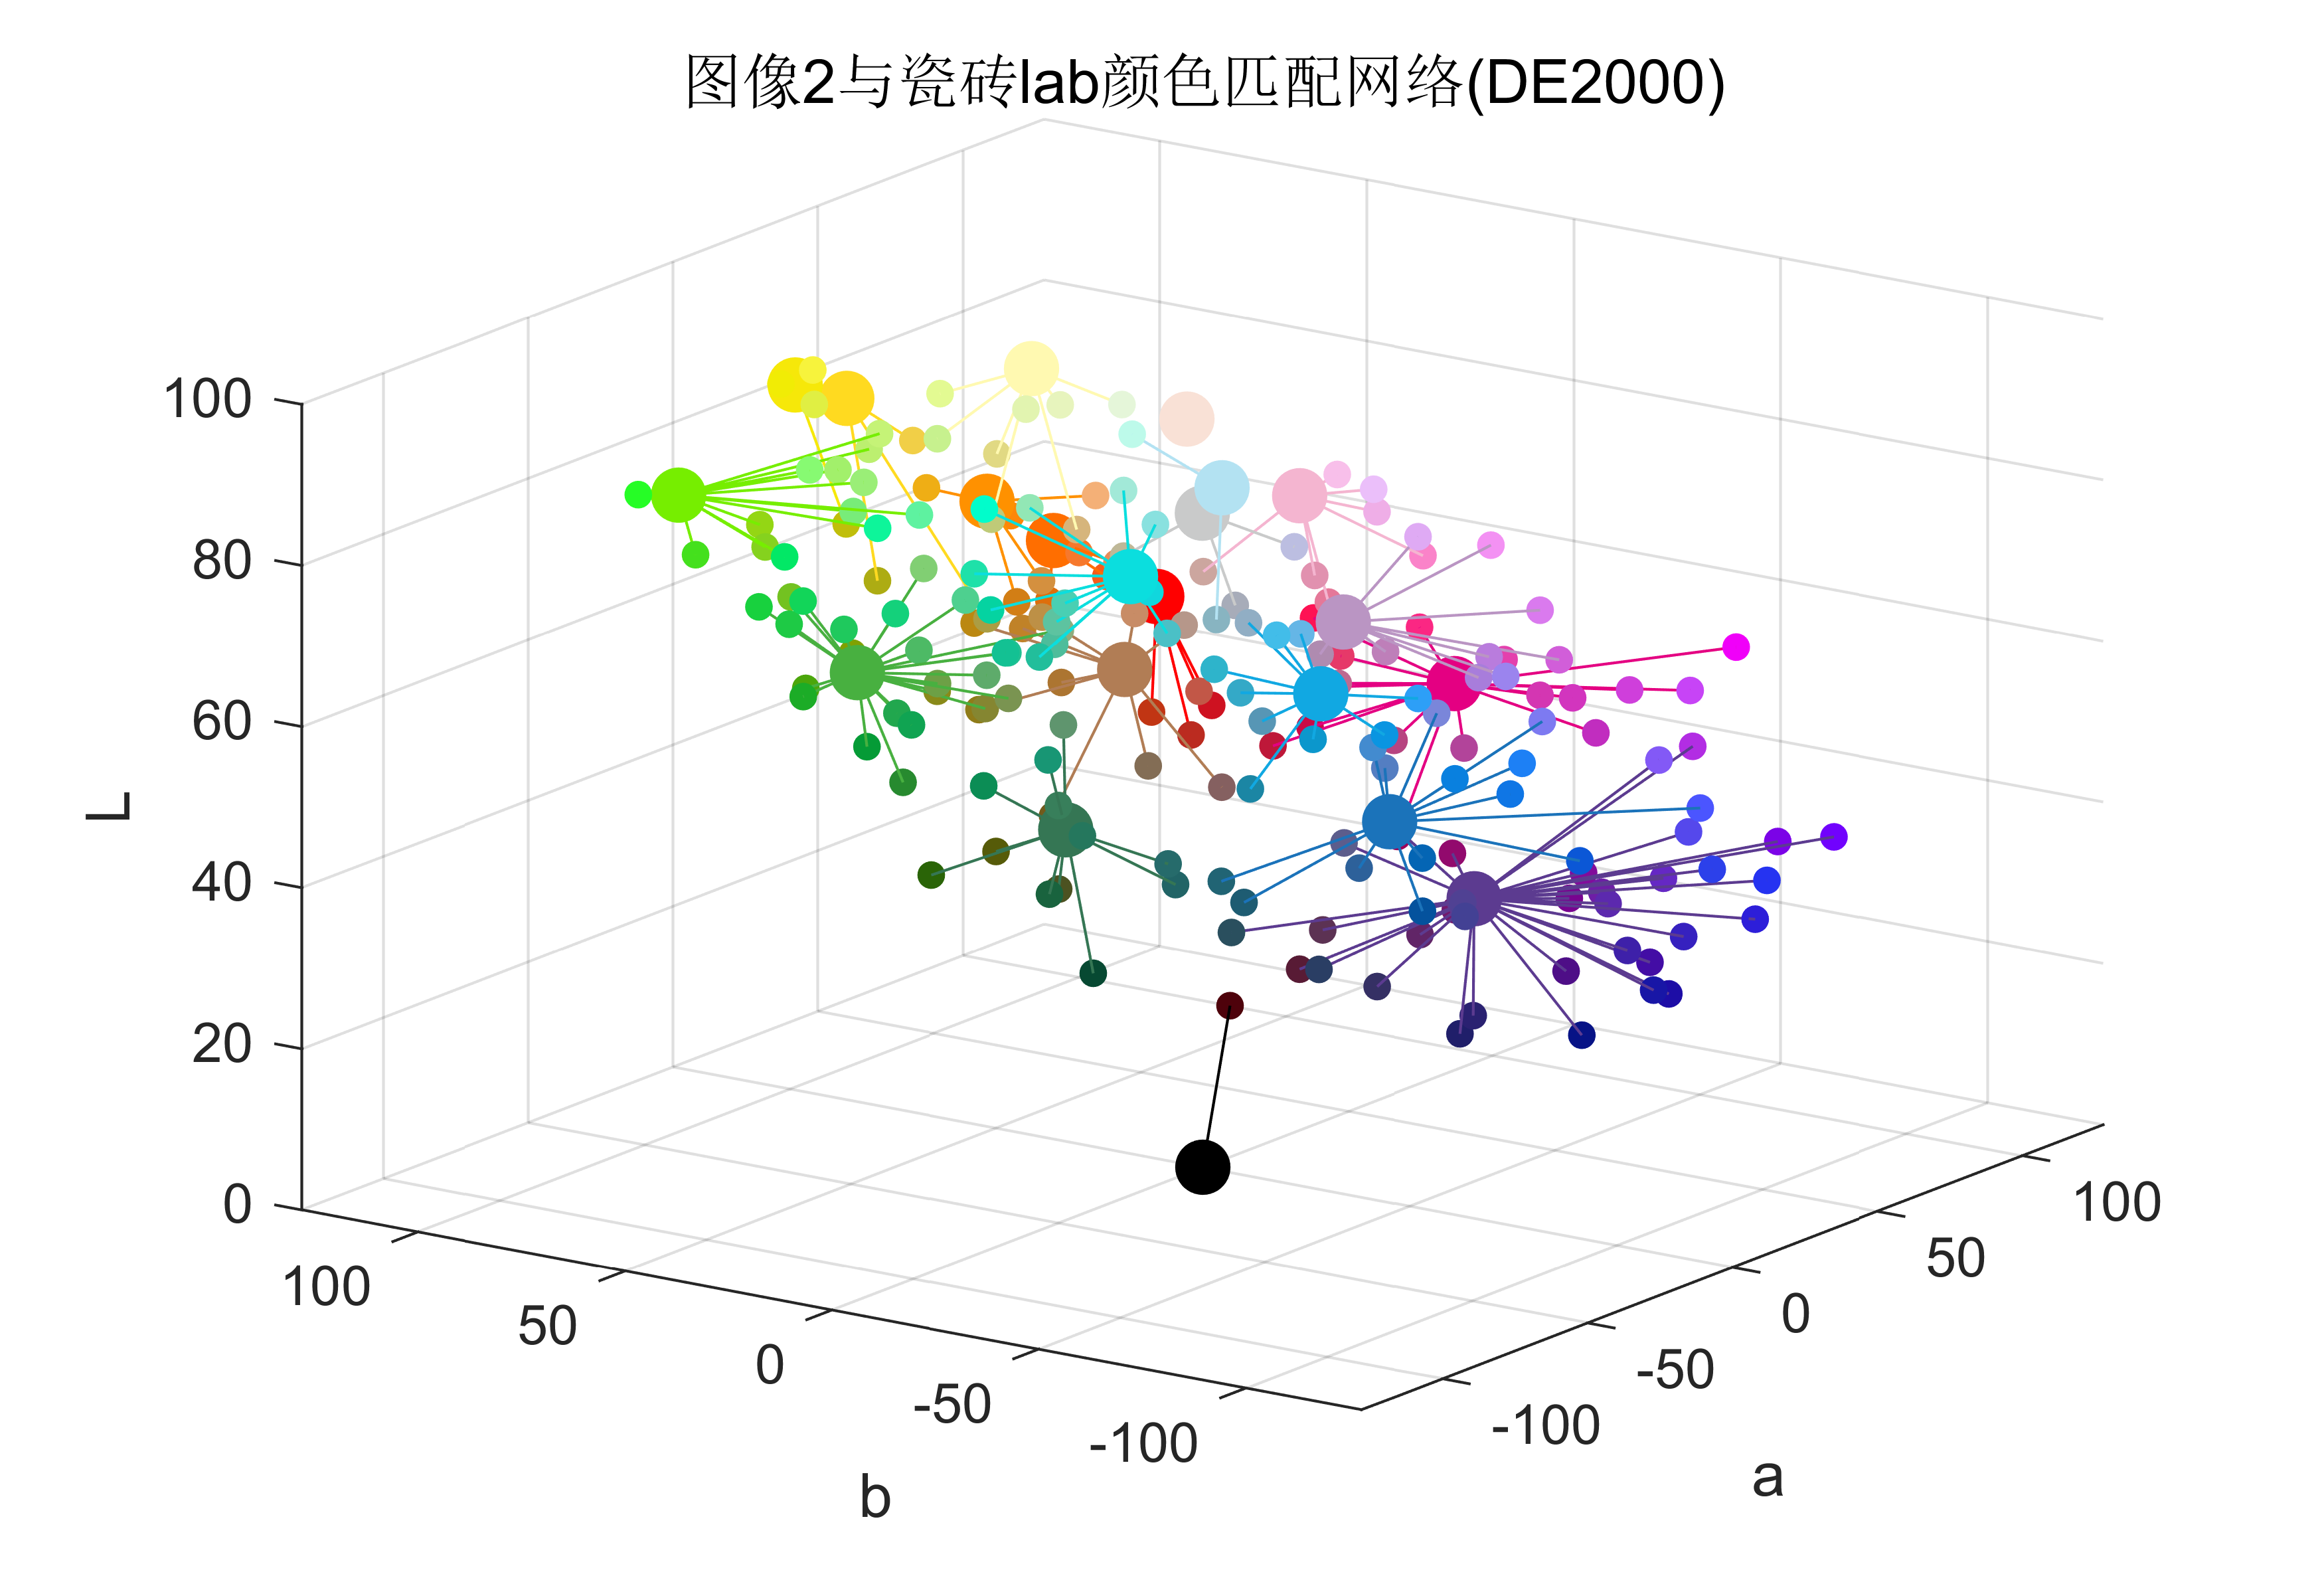
\includegraphics[width=0.47\linewidth]{img/图像2与瓷砖lab颜色匹配网络DE2000.png}
	}
	\caption{图像1,2在LAB空间中的网络连接拓扑图(CIE2000)}
	\label{fig:labcie2000}
\end{figure}
\begin{figure}[H]
	\centering
	\subfigure[图像1的LAB网络连接]{
		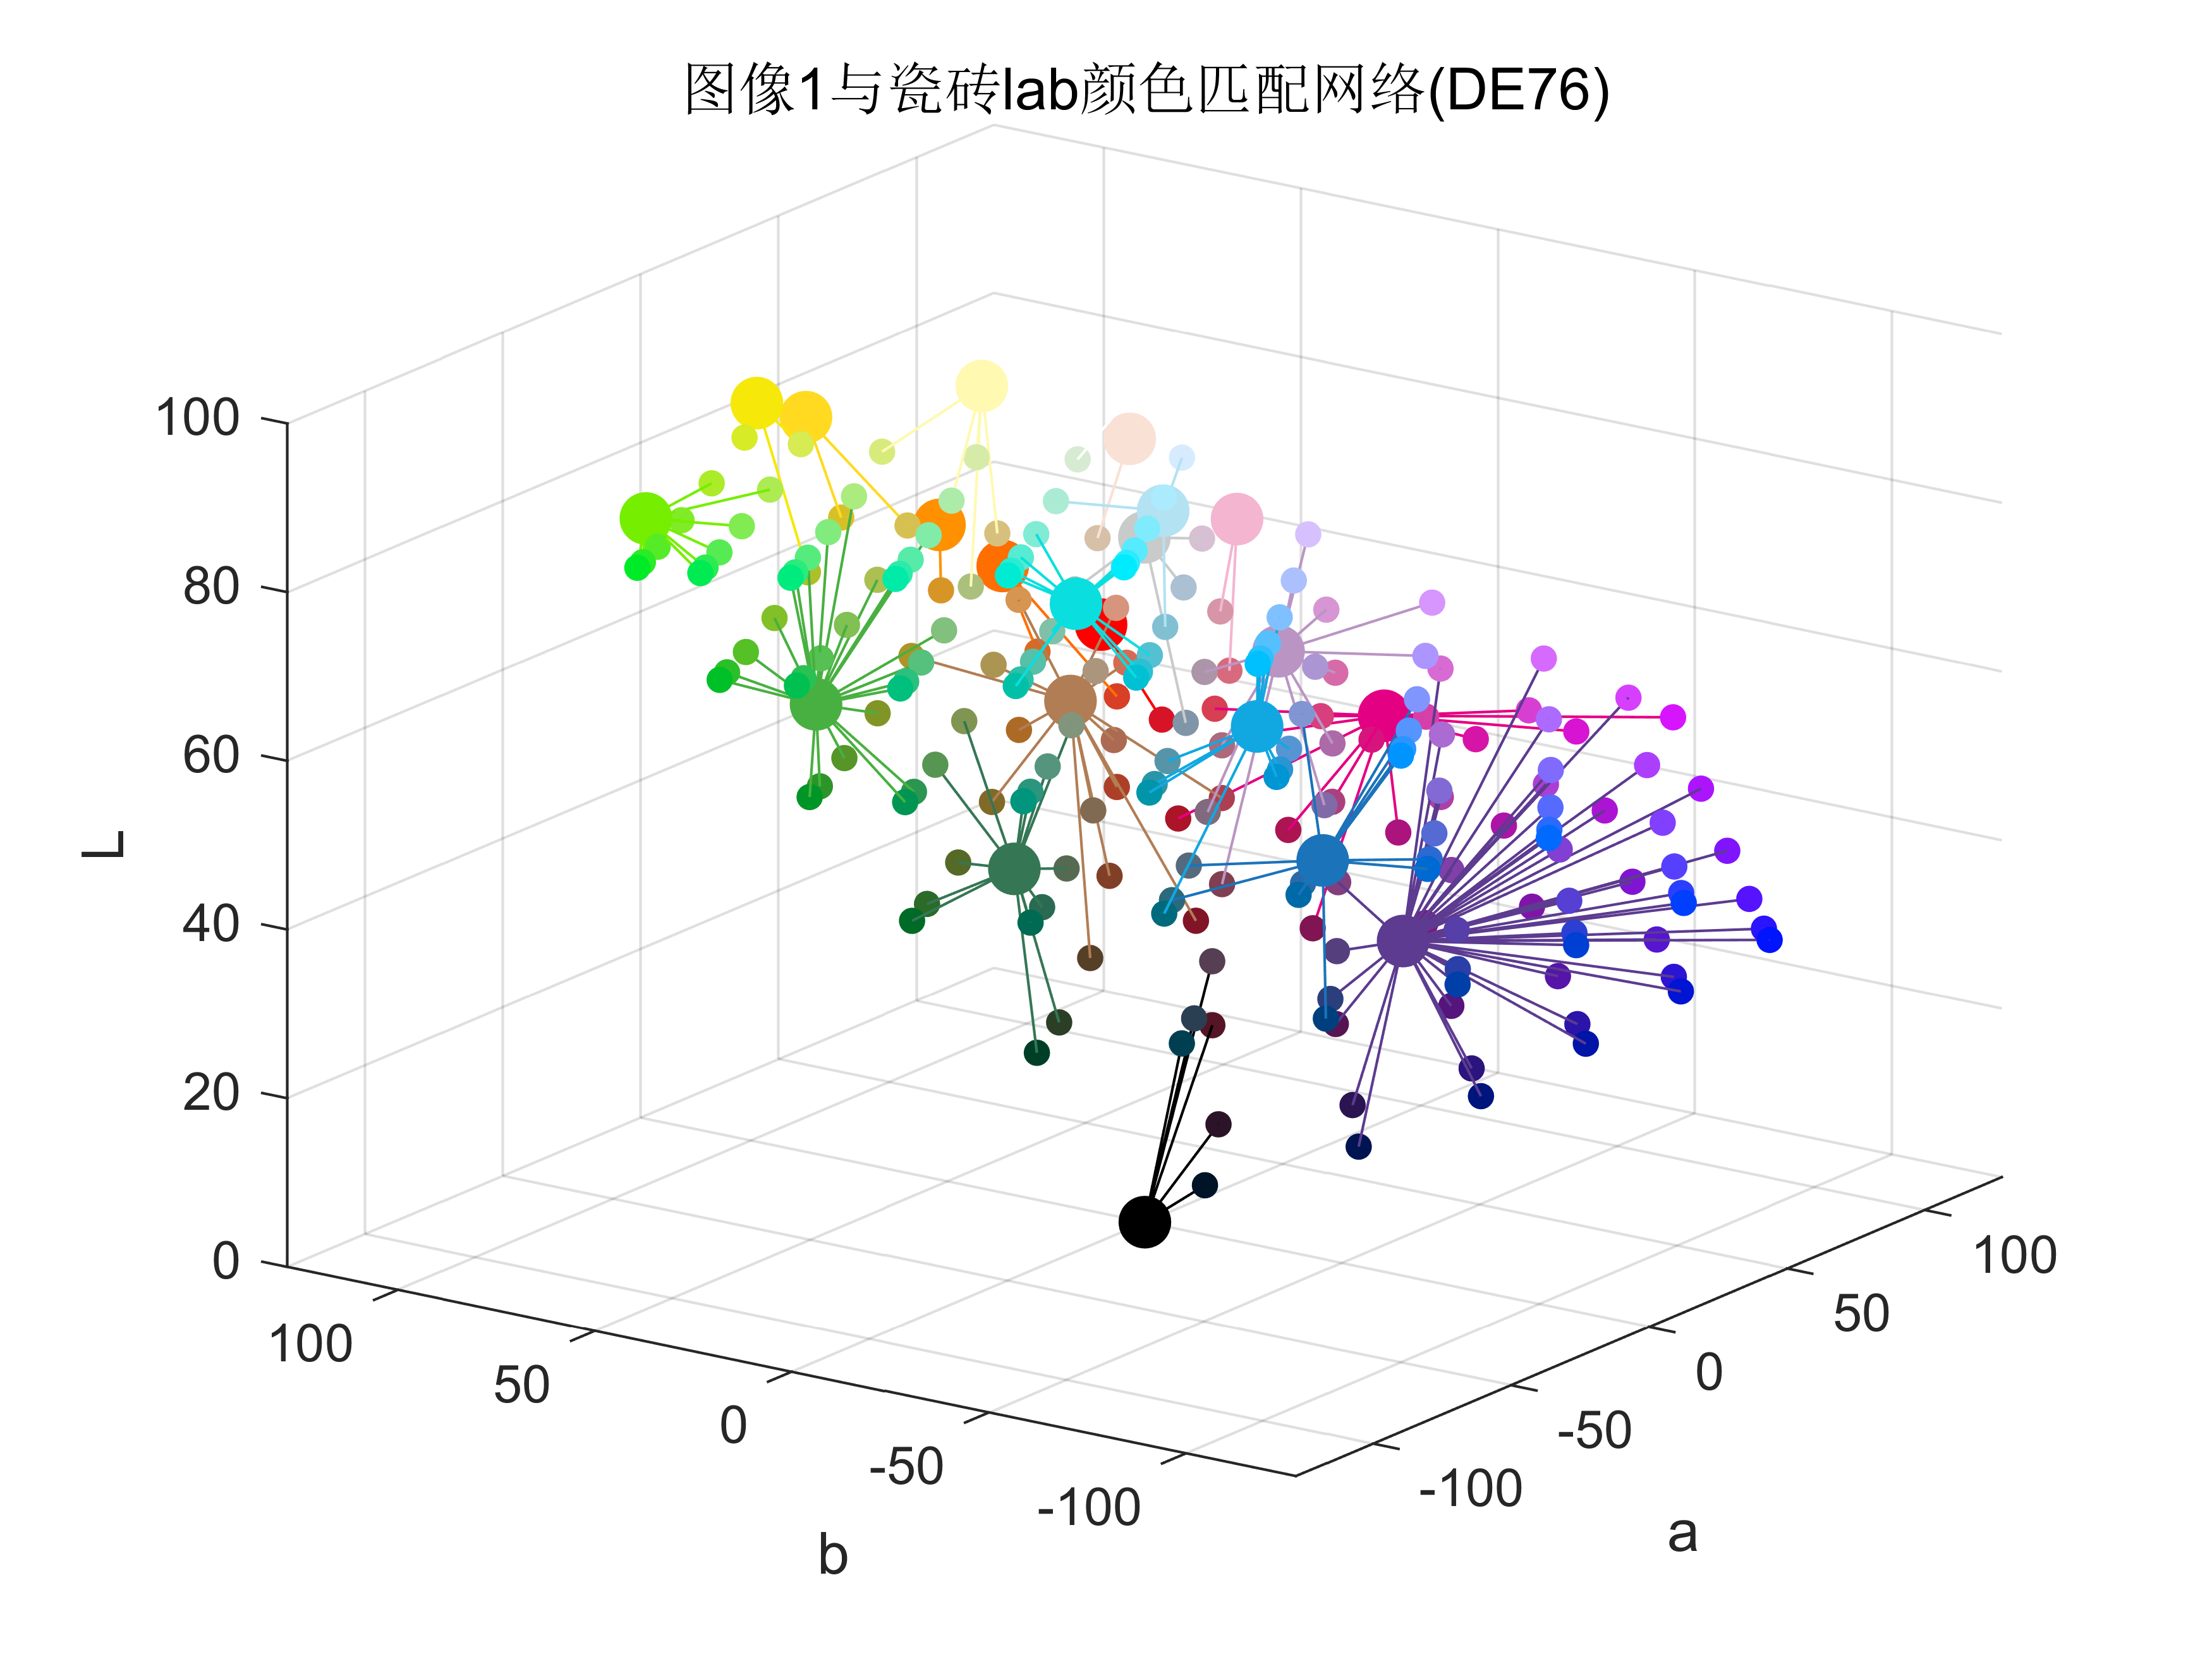
\includegraphics[width=0.47\linewidth]{img/图像1与瓷砖lab颜色匹配网络DE76.png}
		%\caption{fig1}
	}
	\quad
	\subfigure[图像2的LAB网络连接]{
		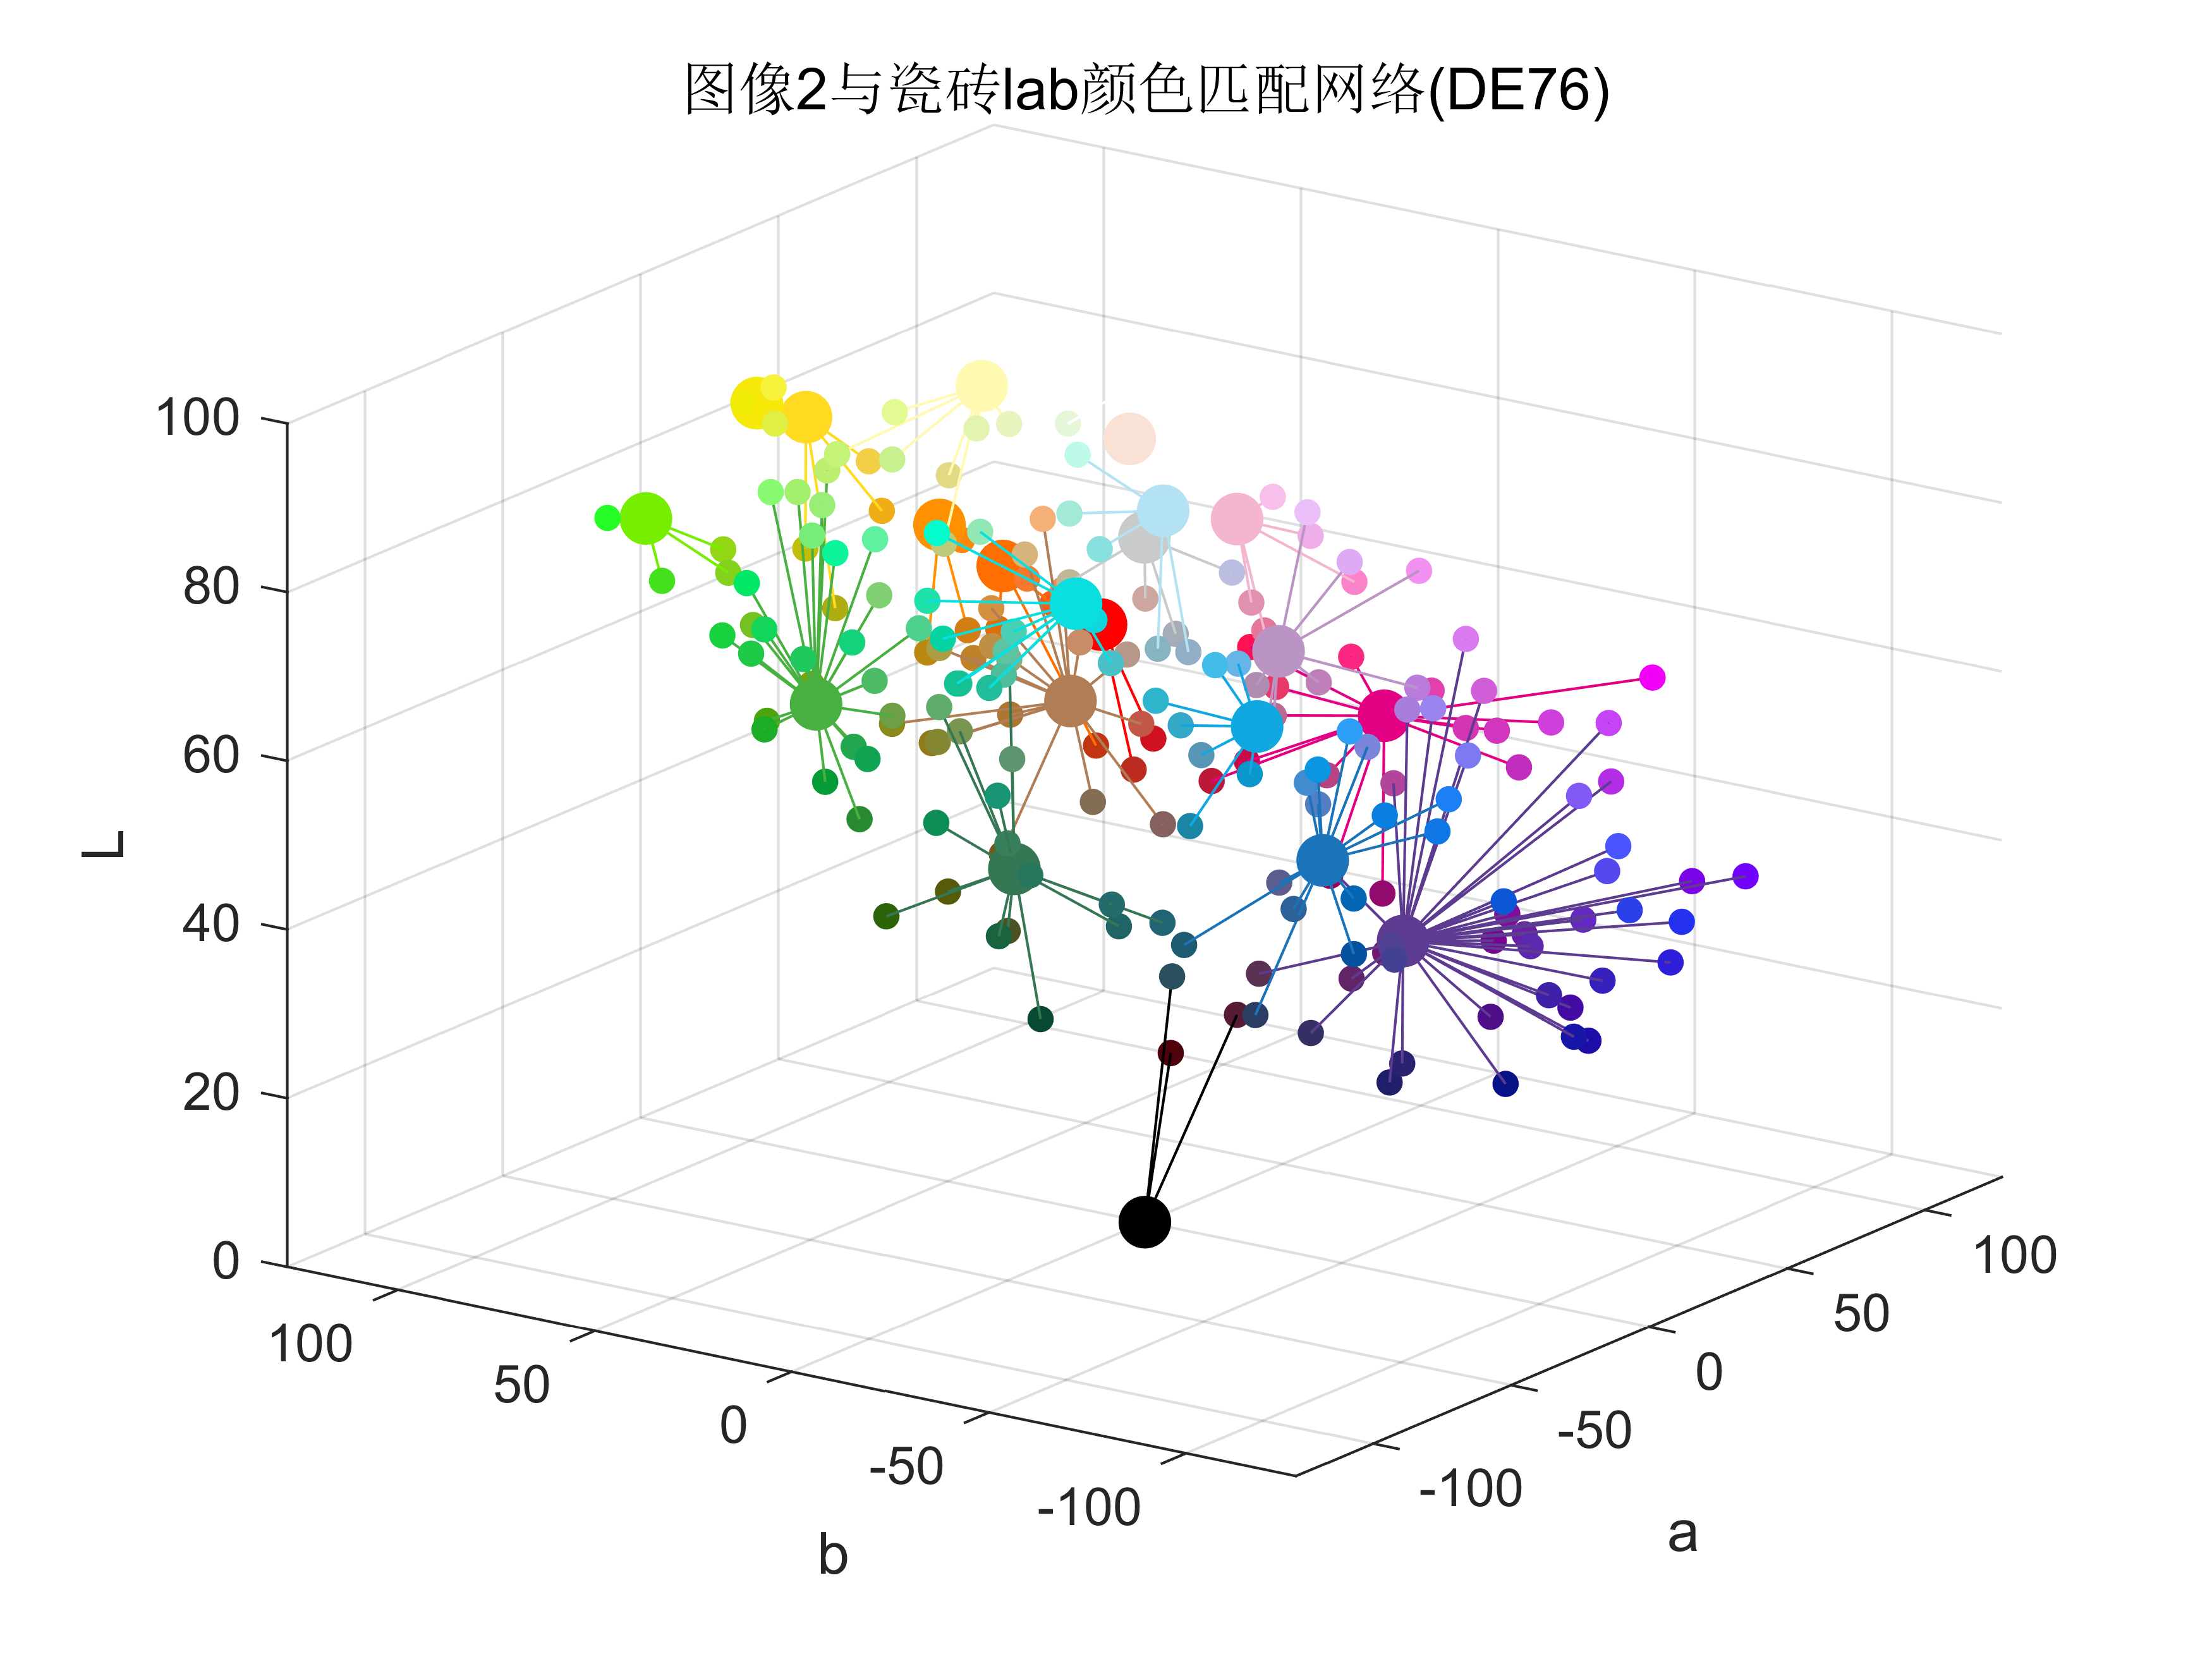
\includegraphics[width=0.47\linewidth]{img/图像2与瓷砖lab颜色匹配网络DE76.png}
	}
	\caption{图像1,2在LAB空间中的网络连接拓扑图(CIE76)}
	\label{fig:labcie76}
\end{figure}
 \section{问题二的求解}
 \subsection{整数规划模型的建立}
 拼接图像的表现力与颜色分布的均匀度有关,颜色分布越均匀,表现力就越强,于是问题转换为:
 
 \textbf{空间中有若干个已知的点,现在要在空间中插入一个或若干个点,使其点的分布尽可能均匀。}
 
 首先,均匀度可以使用公式\eqref{J}(即公式\eqref{j3})表示,均匀度最大,就是要求最小距离的立方和的最大值。
  \begin{equation}
 J \propto  \sum_{i=1}^{n} s_{i}^{3}\,\, ,n\text{为点的数量}
 \label{J}
 \end{equation}
  设需要求解n个点的RGB值,
  \begin{equation}
  \left(R_{i}, G_{i}, B_{i}\right) \quad i=(1,2, \cdots n)+22
  \end{equation}
  已知22个瓷砖颜色点:
  \begin{equation}
  \left[\begin{array}{ccc}
  R_{1}, & G_{1}, & B_{1} \\
  R_{2}, & G_{2},& B_{2} \\
  \vdots & \vdots & \vdots \\
  R_{22}, & G_{22} & B_{22}
  \end{array}\right]
  \end{equation}
  将22个已知点和n个未知点汇合:
   \begin{equation}
  \left[\begin{array}{ccc}
  R_{1}, & G_{1}, & B_{1} \\
  R_{2}, & G_{2},& B_{2} \\
  \vdots & \vdots & \vdots \\
  R_{22}, & G_{22} & B_{22}\\
    R_{i}, & G_{i}, & B_{i} \\
  R_{i+1}, & G_{i+1},& B_{i+1} \\
  \vdots & \vdots & \vdots \\
  R_{n}, & G_{n} & B_{n}
  \end{array}\right]
  \end{equation}
  得到22+n个点:
  \begin{equation}
  \left(R G B_{1}, R G B_{2}, \cdots, R G B_{22}, R G B_{23},\cdots, R G B_{n+22}\right)
  \end{equation}
  矩阵$D$为色差距离矩阵:
  \begin{equation}
  D_{i j}=\triangle E\left(R G B_{i}, R G B_{j}\right)
  \end{equation}
  其中,$\Delta E$为求距离的函数(CIE76,CIE2000或者简化公式),为减小计算复杂度,对问题2的求解使用简化公式\eqref{jianhuags}
  
  目标函数为最小距离立方和,如公式\eqref{mubiao},
  \begin{equation}
  \max : \quad J = \operatorname{Sum}\left([MIN(D)].^{\wedge} 3\right)
  \label{mubiao}
  \end{equation}
  
  其中MIN为求矩阵每行的最小值(即每个点与其最近的点的色差距离),$.^{\wedge} 3$为矩阵对应元素的立方,Sum为求和函数。目标函数值J为均匀度。
  
  约束条件为n个点的整数RGB值在$[0,255]$区间内。
  
  于是建立以下整数规划模型:
  \begin{equation}
  \begin{array}{l}
  \max :\quad J = \operatorname{Sum}\left([MIN(D)].^{\wedge} 3\right) \\
  \text { eq. }\left\{\begin{array}{rl}
  0 \leq R_{i} \leq 255 \\
  0 \leq G_{i} \leq 255 \\
  0 \leq B_{i} \leq 255 \\
  R_{i},G_{i},B_{i} \text{为整数}\\
  i=(1,2, \cdots n)+22
  \end{array}\right.
  \end{array}
  \end{equation}
 \subsection{整数规划模型的求解}
 此问题为NP难问题,由于n较小,依然可以用规划的方法求解。使用Yalmip工具箱和gurobi求解器,设置最大迭代次数,可以在有限时间内获得较好的解。
 
 为减少计算复杂度,目标函数中的方次可以适当减小,可以取距离的和而不是距离立方和。另外,也可以使用遗传算法等启发式算法求解。
 
 设置n分别为1,2,...10,计算目标函数值和对应的RGB值。
 \subsection{求解结果}
 分别设置n的值为0-12,20,求解得到的目标函数值为:
\begin{table}[htbp]
	\centering
	\caption{目标函数值}
	\begin{tabular}{cccccccc}
		\toprule
		\textbf{新增颜色数n} & \textbf{0} & \textbf{1} & \textbf{2} & \textbf{3} & \textbf{4} & \textbf{5} & \textbf{6} \\
		\textbf{目标函数值} & \textbf{124330 } & \textbf{144630 } & \textbf{163340 } & \textbf{178090 } & \textbf{190690 } & \textbf{203150 } & \textbf{214110 } \\
		\midrule
		\textbf{新增颜色数n} & \textbf{7} & \textbf{8} & \textbf{9} & \textbf{10} & \textbf{11} & \textbf{12} & \textbf{20} \\
		\textbf{目标函数值} & \textbf{223260 } & \textbf{235650 } & \textbf{241020 } & \textbf{245410 } & \textbf{249710 } & \textbf{252210 } & \textbf{268720 } \\
		\bottomrule
	\end{tabular}%
	\label{mubiaozhi}%
\end{table}%

增加1个点和增加10个点的散点图如下(大点为新增的点,小点为已经存在的瓷砖RGB点):
   \begin{figure}[H]
	\centering
	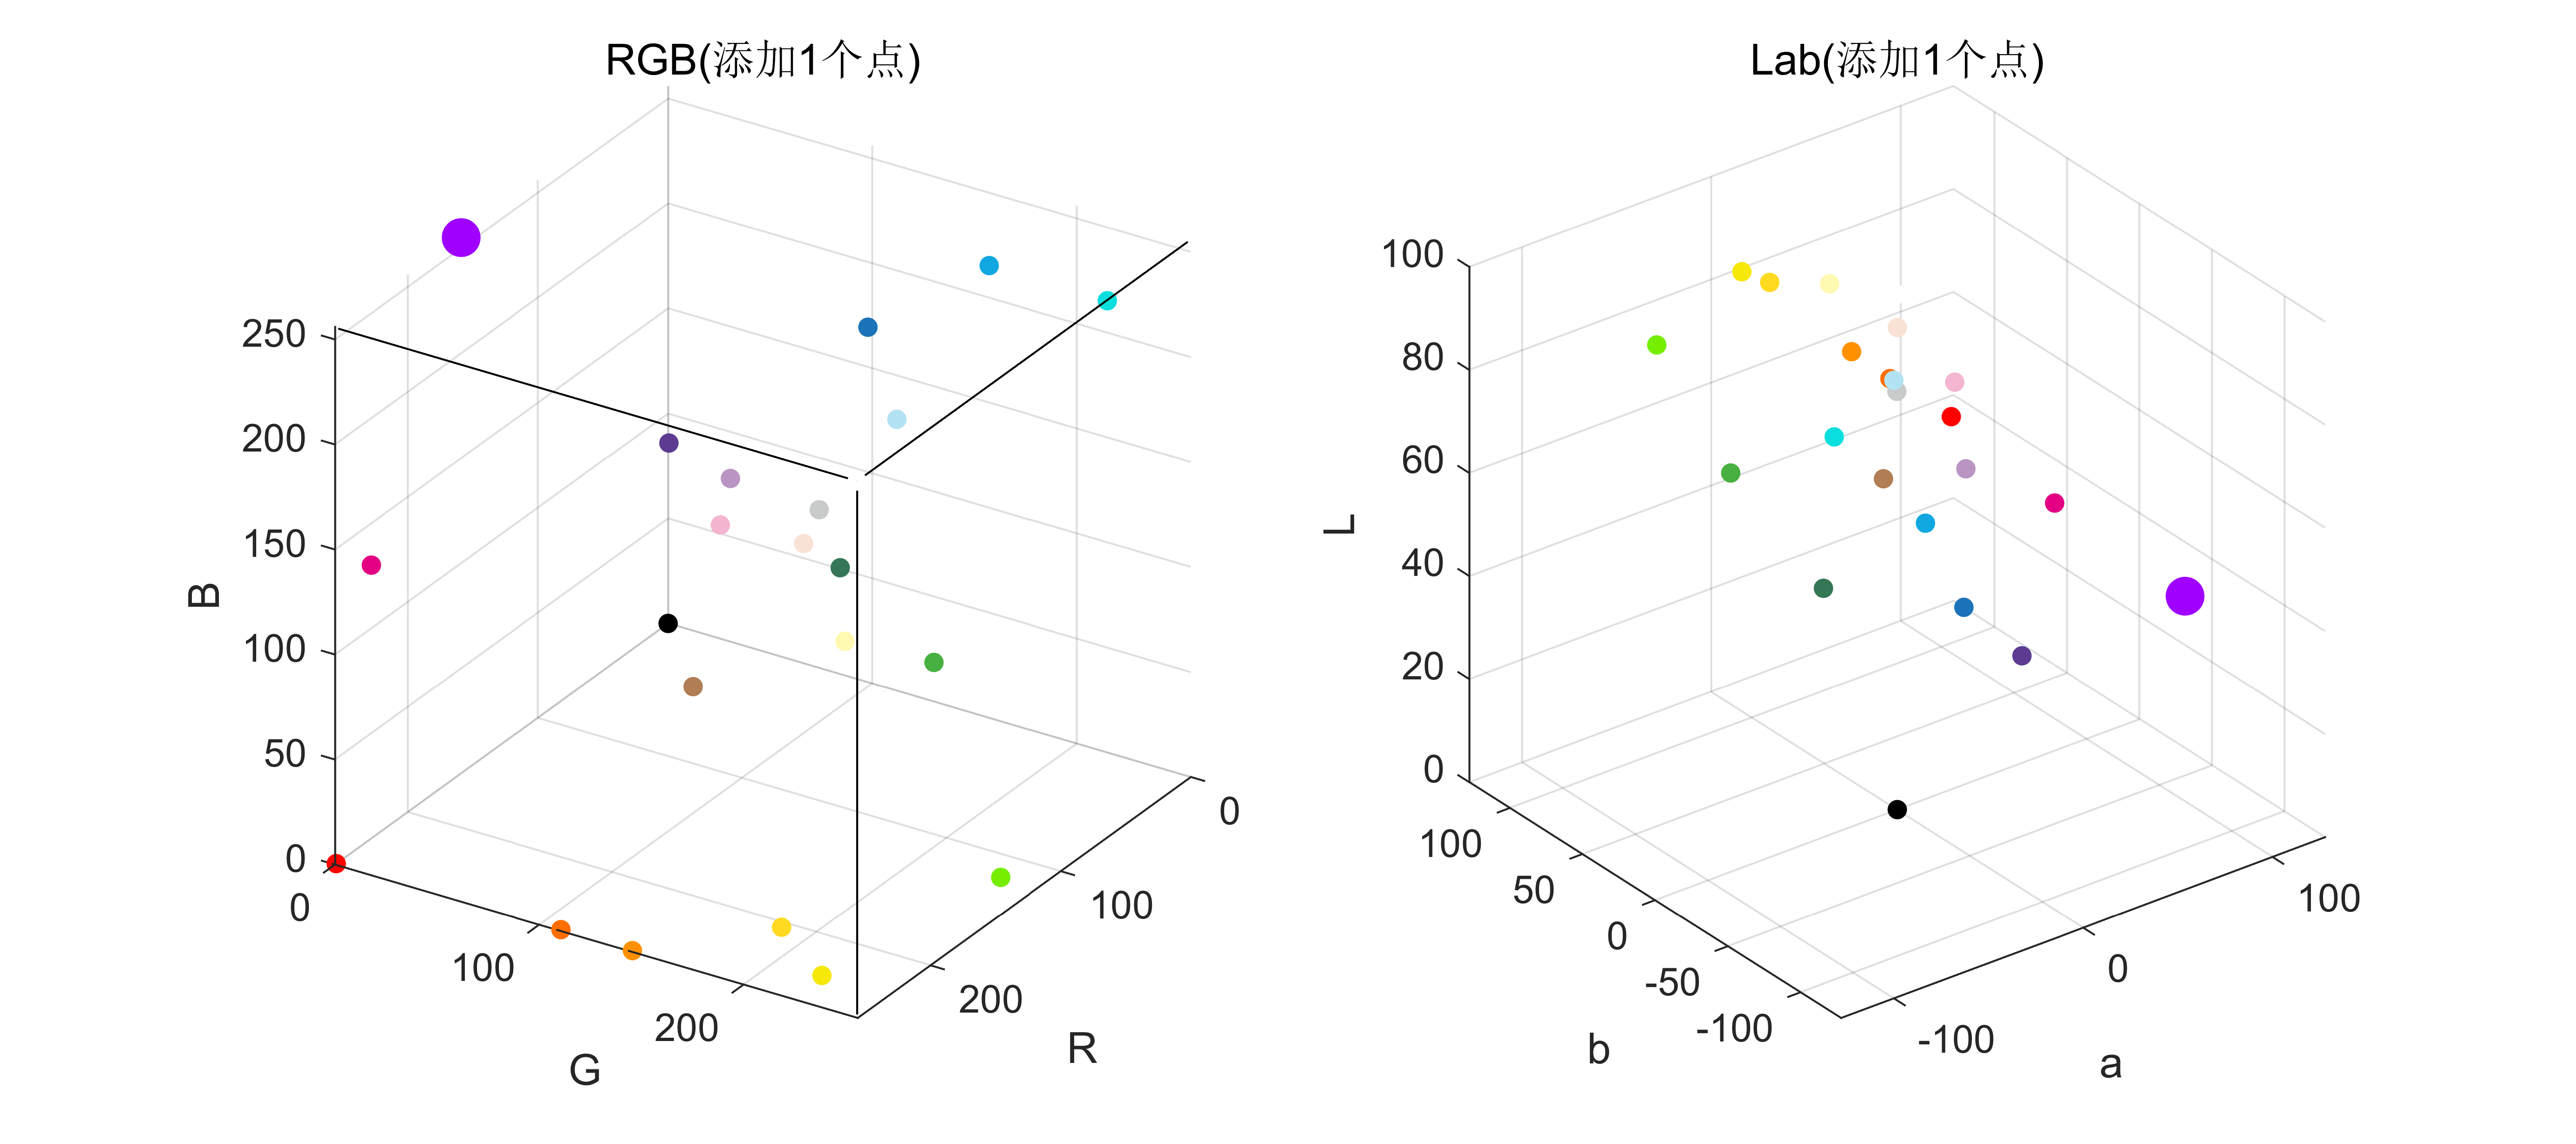
\includegraphics[width=0.95\textwidth]{img/添加1个点.png}
	\caption{添加1个点的RGB和LAB的位置分布}
	\label{添加1个点}
\end{figure}
   \begin{figure}[H]
	\centering
	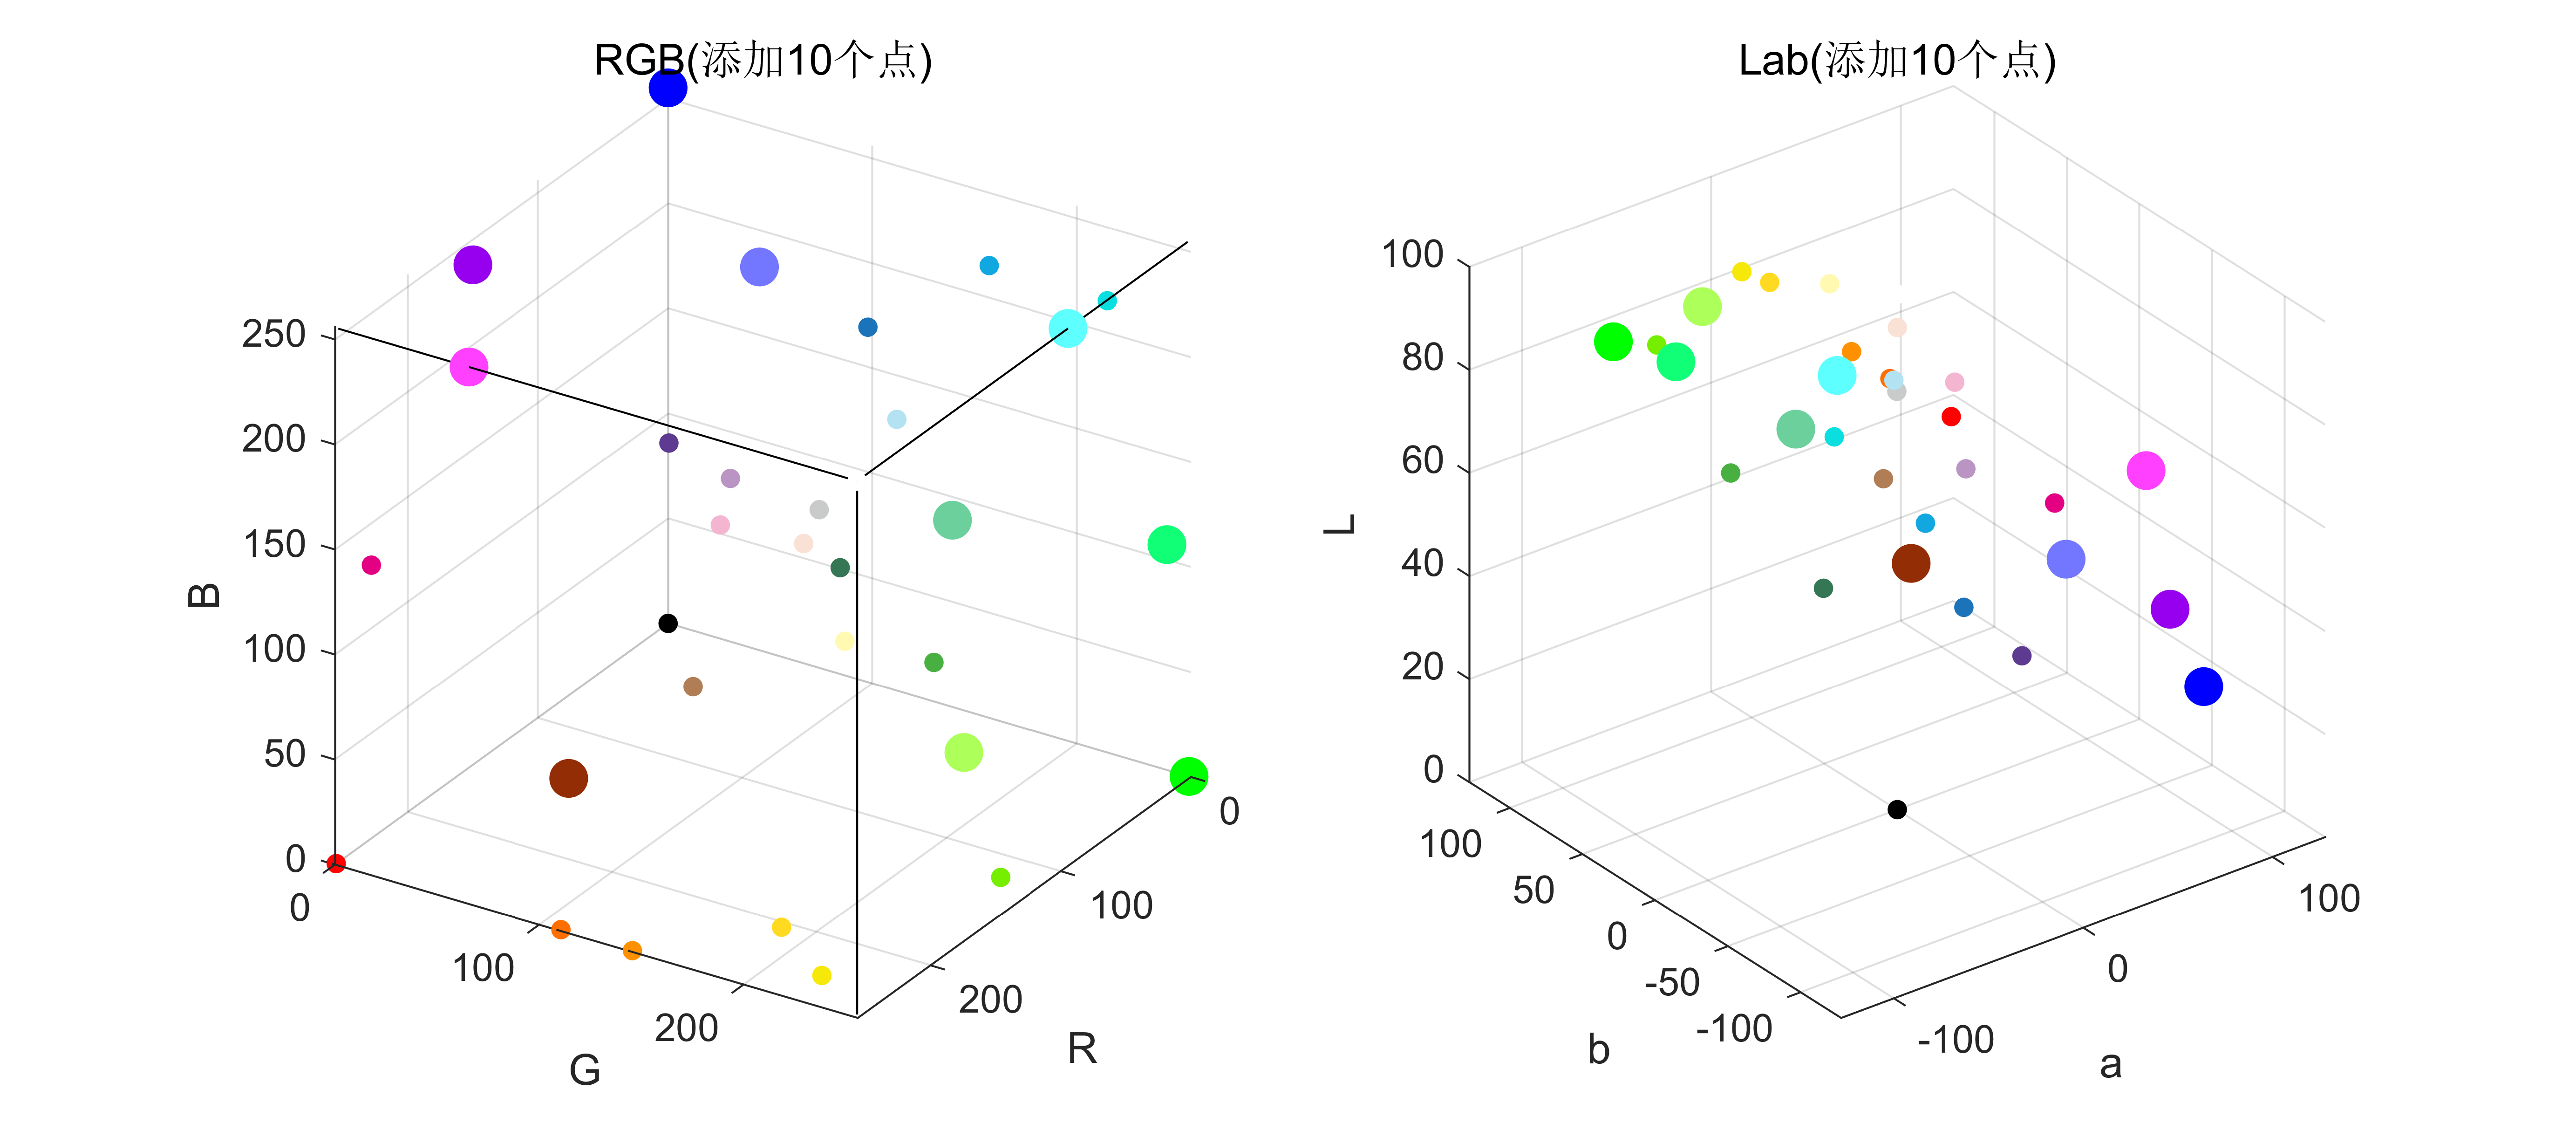
\includegraphics[width=0.95\textwidth]{img/添加10个点.png}
	\caption{添加10个点的RGB和LAB的位置分布}
	\label{添加10个点}
\end{figure}

具体的RGB值和颜色如表3,由表中颜色分布可见,新增的颜色分布较均匀,模型求解的效果较好:
\begin{table}[H]
	\centering
	\caption{增加的RGB值}
	\begin{tabular}{|ccccc|r|ccccr|r|ccccc|}
		\multicolumn{5}{c}{\textbf{增加1种}}     & \multicolumn{1}{r}{} & \multicolumn{5}{c}{\textbf{增加5种}}     & \multicolumn{1}{r}{} & \multicolumn{5}{c}{\textbf{增加8种}} \\
		\cmidrule{1-5}\cmidrule{7-11}\cmidrule{13-17}    \textbf{序号} & \textbf{R} & \textbf{G} & \textbf{B} &       &       & \textbf{序号} & \textbf{R} & \textbf{G} & \textbf{B} &       &       & \textbf{序号} & \textbf{R} & \textbf{G} & \textbf{B} &  \\
		\textbf{1} & \textbf{159} & \textbf{0} & \textbf{255} & \cellcolor[rgb]{ .624,  0,  1} &       & \textbf{1} & \textbf{159} & \textbf{0} & \textbf{255} & \cellcolor[rgb]{ .624,  0,  1} &       & \textbf{1} & \textbf{145} & \textbf{43} & \textbf{5} & \cellcolor[rgb]{ .569,  .169,  .02} \\
		\cmidrule{1-5}    \multicolumn{1}{r}{} &       &       &       & \multicolumn{1}{r}{} &       & \textbf{2} & \textbf{0} & \textbf{255} & \textbf{117} & \cellcolor[rgb]{ 0,  1,  .459} &       & \textbf{2} & \textbf{255} & \textbf{51} & \textbf{250} & \cellcolor[rgb]{ 1,  .2,  .98} \\
		\multicolumn{1}{r}{} &       &       &       & \multicolumn{1}{r}{} &       & \textbf{3} & \textbf{0} & \textbf{0} & \textbf{255} & \cellcolor[rgb]{ 0,  0,  1} &       & \textbf{3} & \textbf{34} & \textbf{255} & \textbf{124} & \cellcolor[rgb]{ .133,  1,  .486} \\
		\multicolumn{1}{r}{} &       &       &       & \multicolumn{1}{r}{} &       & \textbf{4} & \textbf{143} & \textbf{255} & \textbf{114} & \cellcolor[rgb]{ .561,  1,  .447} &       & \textbf{4} & \textbf{106} & \textbf{183} & \textbf{223} & \cellcolor[rgb]{ .416,  .718,  .875} \\
		\multicolumn{1}{r}{} &       &       &       & \multicolumn{1}{r}{} &       & \textbf{5} & \textbf{0} & \textbf{245} & \textbf{0} & \cellcolor[rgb]{ 0,  .961,  0} &       & \textbf{5} & \textbf{134} & \textbf{0} & \textbf{255} & \cellcolor[rgb]{ .525,  0,  1} \\
		\cmidrule{7-11}    \multicolumn{5}{c}{\textbf{增加2种}}     & \multicolumn{1}{r}{} &       &       &       &       & \multicolumn{1}{r}{} &       & \textbf{6} & \textbf{0} & \textbf{255} & \textbf{9} & \cellcolor[rgb]{ 0,  1,  .035} \\
		\cmidrule{1-5}    \textbf{序号} & \textbf{R} & \textbf{G} & \textbf{B} &       & \multicolumn{1}{r}{} &       &       &       &       & \multicolumn{1}{r}{} &       & \textbf{7} & \textbf{171} & \textbf{247} & \textbf{102} & \cellcolor[rgb]{ .671,  .969,  .4} \\
		\textbf{1} & \textbf{0} & \textbf{0} & \textbf{255} & \cellcolor[rgb]{ 0,  0,  1} & \multicolumn{1}{r}{} &       &       &       &       & \multicolumn{1}{r}{} &       & \textbf{8} & \textbf{0} & \textbf{2} & \textbf{255} & \cellcolor[rgb]{ 0,  .008,  1} \\
		\cmidrule{13-17}    \textbf{2} & \textbf{159} & \textbf{0} & \textbf{255} & \cellcolor[rgb]{ .624,  0,  1} & \multicolumn{1}{r}{} &       &       &       &       & \multicolumn{1}{r}{} & \multicolumn{1}{r}{} & \multicolumn{5}{c}{\textbf{增加9种}} \\
		\cmidrule{1-5}\cmidrule{13-17}    \multicolumn{1}{r}{} &       &       &       & \multicolumn{1}{r}{} & \multicolumn{1}{r}{} & \multicolumn{5}{c}{\textbf{增加6种}}     &       & \textbf{序号} & \textbf{R} & \textbf{G} & \textbf{B} &  \\
		\cmidrule{7-11}    \multicolumn{1}{r}{} &       &       &       & \multicolumn{1}{r}{} &       & \textbf{序号} & \textbf{R} & \textbf{G} & \textbf{B} &       &       & \textbf{1} & \textbf{147} & \textbf{48} & \textbf{0} & \cellcolor[rgb]{ .576,  .188,  0} \\
		\multicolumn{1}{r}{} &       &       &       & \multicolumn{1}{r}{} &       & \textbf{1} & \textbf{132} & \textbf{0} & \textbf{255} & \cellcolor[rgb]{ .518,  0,  1} &       & \textbf{2} & \textbf{255} & \textbf{47} & \textbf{253} & \cellcolor[rgb]{ 1,  .184,  .992} \\
		\multicolumn{1}{r}{} &       &       &       & \multicolumn{1}{r}{} &       & \textbf{2} & \textbf{0} & \textbf{255} & \textbf{10} & \cellcolor[rgb]{ 0,  1,  .039} &       & \textbf{3} & \textbf{173} & \textbf{243} & \textbf{103} & \cellcolor[rgb]{ .678,  .953,  .404} \\
		\multicolumn{1}{c}{} &       &       &       & \multicolumn{1}{c}{} &       & \textbf{3} & \textbf{0} & \textbf{0} & \textbf{246} & \cellcolor[rgb]{ 0,  0,  .965} &       & \textbf{4} & \textbf{0} & \textbf{0} & \textbf{255} & \cellcolor[rgb]{ 0,  0,  1} \\
		\multicolumn{1}{c}{} &       &       &       & \multicolumn{1}{c}{} &       & \textbf{4} & \textbf{113} & \textbf{134} & \textbf{255} & \cellcolor[rgb]{ .443,  .525,  1} &       & \textbf{5} & \textbf{123} & \textbf{72} & \textbf{255} & \cellcolor[rgb]{ .482,  .282,  1} \\
		\multicolumn{5}{c}{\textbf{增加3种}}     &       & \textbf{5} & \textbf{255} & \textbf{47} & \textbf{251} & \cellcolor[rgb]{ 1,  .184,  .984} &       & \textbf{6} & \textbf{106} & \textbf{182} & \textbf{185} & \cellcolor[rgb]{ .416,  .714,  .725} \\
		\cmidrule{1-5}    \textbf{序号} & \textbf{R} & \textbf{G} & \textbf{B} &       &       & \textbf{6} & \textbf{103} & \textbf{250} & \textbf{152} & \cellcolor[rgb]{ .404,  .98,  .596} &       & \textbf{7} & \textbf{0} & \textbf{255} & \textbf{10} & \cellcolor[rgb]{ 0,  1,  .039} \\
		\cmidrule{7-11}    \textbf{1} & \textbf{0} & \textbf{0} & \textbf{255} & \cellcolor[rgb]{ 0,  0,  1} & \multicolumn{1}{r}{} &       &       &       &       & \multicolumn{1}{r}{} &       & \textbf{8} & \textbf{67} & \textbf{255} & \textbf{136} & \cellcolor[rgb]{ .263,  1,  .533} \\
		\textbf{2} & \textbf{104} & \textbf{255} & \textbf{151} & \cellcolor[rgb]{ .408,  1,  .592} & \multicolumn{1}{r}{} &       &       &       &       & \multicolumn{1}{r}{} &       & \textbf{9} & \textbf{0} & \textbf{187} & \textbf{126} & \cellcolor[rgb]{ 0,  .733,  .494} \\
		\cmidrule{13-17}    \textbf{3} & \textbf{159} & \textbf{0} & \textbf{255} & \cellcolor[rgb]{ .624,  0,  1} & \multicolumn{1}{r}{} &       &       &       &       & \multicolumn{1}{r}{} & \multicolumn{1}{r}{} & \multicolumn{5}{c}{\textbf{增加10种}} \\
		\cmidrule{1-5}\cmidrule{13-17}    \multicolumn{1}{r}{} &       &       &       & \multicolumn{1}{r}{} & \multicolumn{1}{r}{} &       &       &       &       & \multicolumn{1}{r}{} &       & \textbf{序号} & \textbf{R} & \textbf{G} & \textbf{B} &  \\
		\multicolumn{1}{r}{} &       &       &       & \multicolumn{1}{r}{} & \multicolumn{1}{r}{} &       &       &       &       & \multicolumn{1}{r}{} &       & \textbf{1} & \textbf{93} & \textbf{255} & \textbf{255} & \cellcolor[rgb]{ .365,  1,  1} \\
		\multicolumn{1}{r}{} &       &       &       & \multicolumn{1}{r}{} & \multicolumn{1}{r}{} & \multicolumn{5}{c}{\textbf{增加7种}}     &       & \textbf{2} & \textbf{255} & \textbf{65} & \textbf{255} & \cellcolor[rgb]{ 1,  .255,  1} \\
		\cmidrule{7-11}    \multicolumn{1}{r}{} &       &       &       & \multicolumn{1}{r}{} &       & \textbf{序号} & \textbf{R} & \textbf{G} & \textbf{B} &       &       & \textbf{3} & \textbf{17} & \textbf{255} & \textbf{118} & \cellcolor[rgb]{ .067,  1,  .463} \\
		\multicolumn{1}{r}{} &       &       &       & \multicolumn{1}{r}{} &       & \textbf{1} & \textbf{159} & \textbf{0} & \textbf{255} & \cellcolor[rgb]{ .624,  0,  1} &       & \textbf{4} & \textbf{150} & \textbf{0} & \textbf{238} & \cellcolor[rgb]{ .588,  0,  .933} \\
		\multicolumn{5}{c}{\textbf{增加4种}}     &       & \textbf{2} & \textbf{146} & \textbf{48} & \textbf{0} & \cellcolor[rgb]{ .573,  .188,  0} &       & \textbf{5} & \textbf{147} & \textbf{45} & \textbf{5} & \cellcolor[rgb]{ .576,  .176,  .02} \\
		\cmidrule{1-5}    \textbf{序号} & \textbf{R} & \textbf{G} & \textbf{B} &       &       & \textbf{3} & \textbf{105} & \textbf{255} & \textbf{220} & \cellcolor[rgb]{ .412,  1,  .863} &       & \textbf{6} & \textbf{0} & \textbf{0} & \textbf{255} & \cellcolor[rgb]{ 0,  0,  1} \\
		\textbf{1} & \textbf{0} & \textbf{0} & \textbf{255} & \cellcolor[rgb]{ 0,  0,  1} &       & \textbf{4} & \textbf{11} & \textbf{255} & \textbf{115} & \cellcolor[rgb]{ .043,  1,  .451} &       & \textbf{7} & \textbf{0} & \textbf{255} & \textbf{0} & \cellcolor[rgb]{ 0,  1,  0} \\
		\textbf{2} & \textbf{179} & \textbf{26} & \textbf{255} & \cellcolor[rgb]{ .702,  .102,  1} &       & \textbf{5} & \textbf{141} & \textbf{255} & \textbf{111} & \cellcolor[rgb]{ .553,  1,  .435} &       & \textbf{8} & \textbf{173} & \textbf{255} & \textbf{89} & \cellcolor[rgb]{ .678,  1,  .349} \\
		\textbf{3} & \textbf{0} & \textbf{255} & \textbf{0} & \cellcolor[rgb]{ 0,  1,  0} &       & \textbf{6} & \textbf{0} & \textbf{243} & \textbf{0} & \cellcolor[rgb]{ 0,  .953,  0} &       & \textbf{9} & \textbf{108} & \textbf{208} & \textbf{157} & \cellcolor[rgb]{ .424,  .816,  .616} \\
		\textbf{4} & \textbf{105} & \textbf{255} & \textbf{150} & \cellcolor[rgb]{ .412,  1,  .588} &       & \textbf{7} & \textbf{0} & \textbf{0} & \textbf{255} & \cellcolor[rgb]{ 0,  0,  1} &       & \textbf{10} & \textbf{115} & \textbf{118} & \textbf{255} & \cellcolor[rgb]{ .451,  .463,  1} \\
		\cmidrule{1-5}\cmidrule{7-11}\cmidrule{13-17}    \end{tabular}%
	\label{wt2fb}%
\end{table}%

 
 
 \section{问题三的求解}
 \subsection{表现力随新增颜色数量的关系}
 由假设2,表现力随新增颜色数量的增大而增大,且增速逐渐减小,并且趋于一个极限值。该假设基于这样一条现实:当颜色足够多时,表现力已经很大,继续增加颜色没有意义。
 因此可以用一个函数拟合表现力随新增颜色数量的关系,表现力即问题二中求得的目标函数值,目标函数值越大说明表现力越强。
 
 需要找到一个递增的函数,且随着自变量的增大,斜率逐渐变小,并最终趋于一个极限值。显然,这个函数可以是
   \begin{equation}
  f(x)=\frac{a x + b}{c x + d}
 \end{equation}
 对表\ref{mubiaozhi}的数据进行归一到$[0,1]$区间,用归一化的数据进行拟合,得到$a=1.459,b=-0.1841,c=1,d=7.622$,即;
    \begin{equation}
 f(n)=\frac{1.459 n -0.1841}{ n + 7.622}
 \end{equation}
    \begin{figure}[H]
 	\centering
 	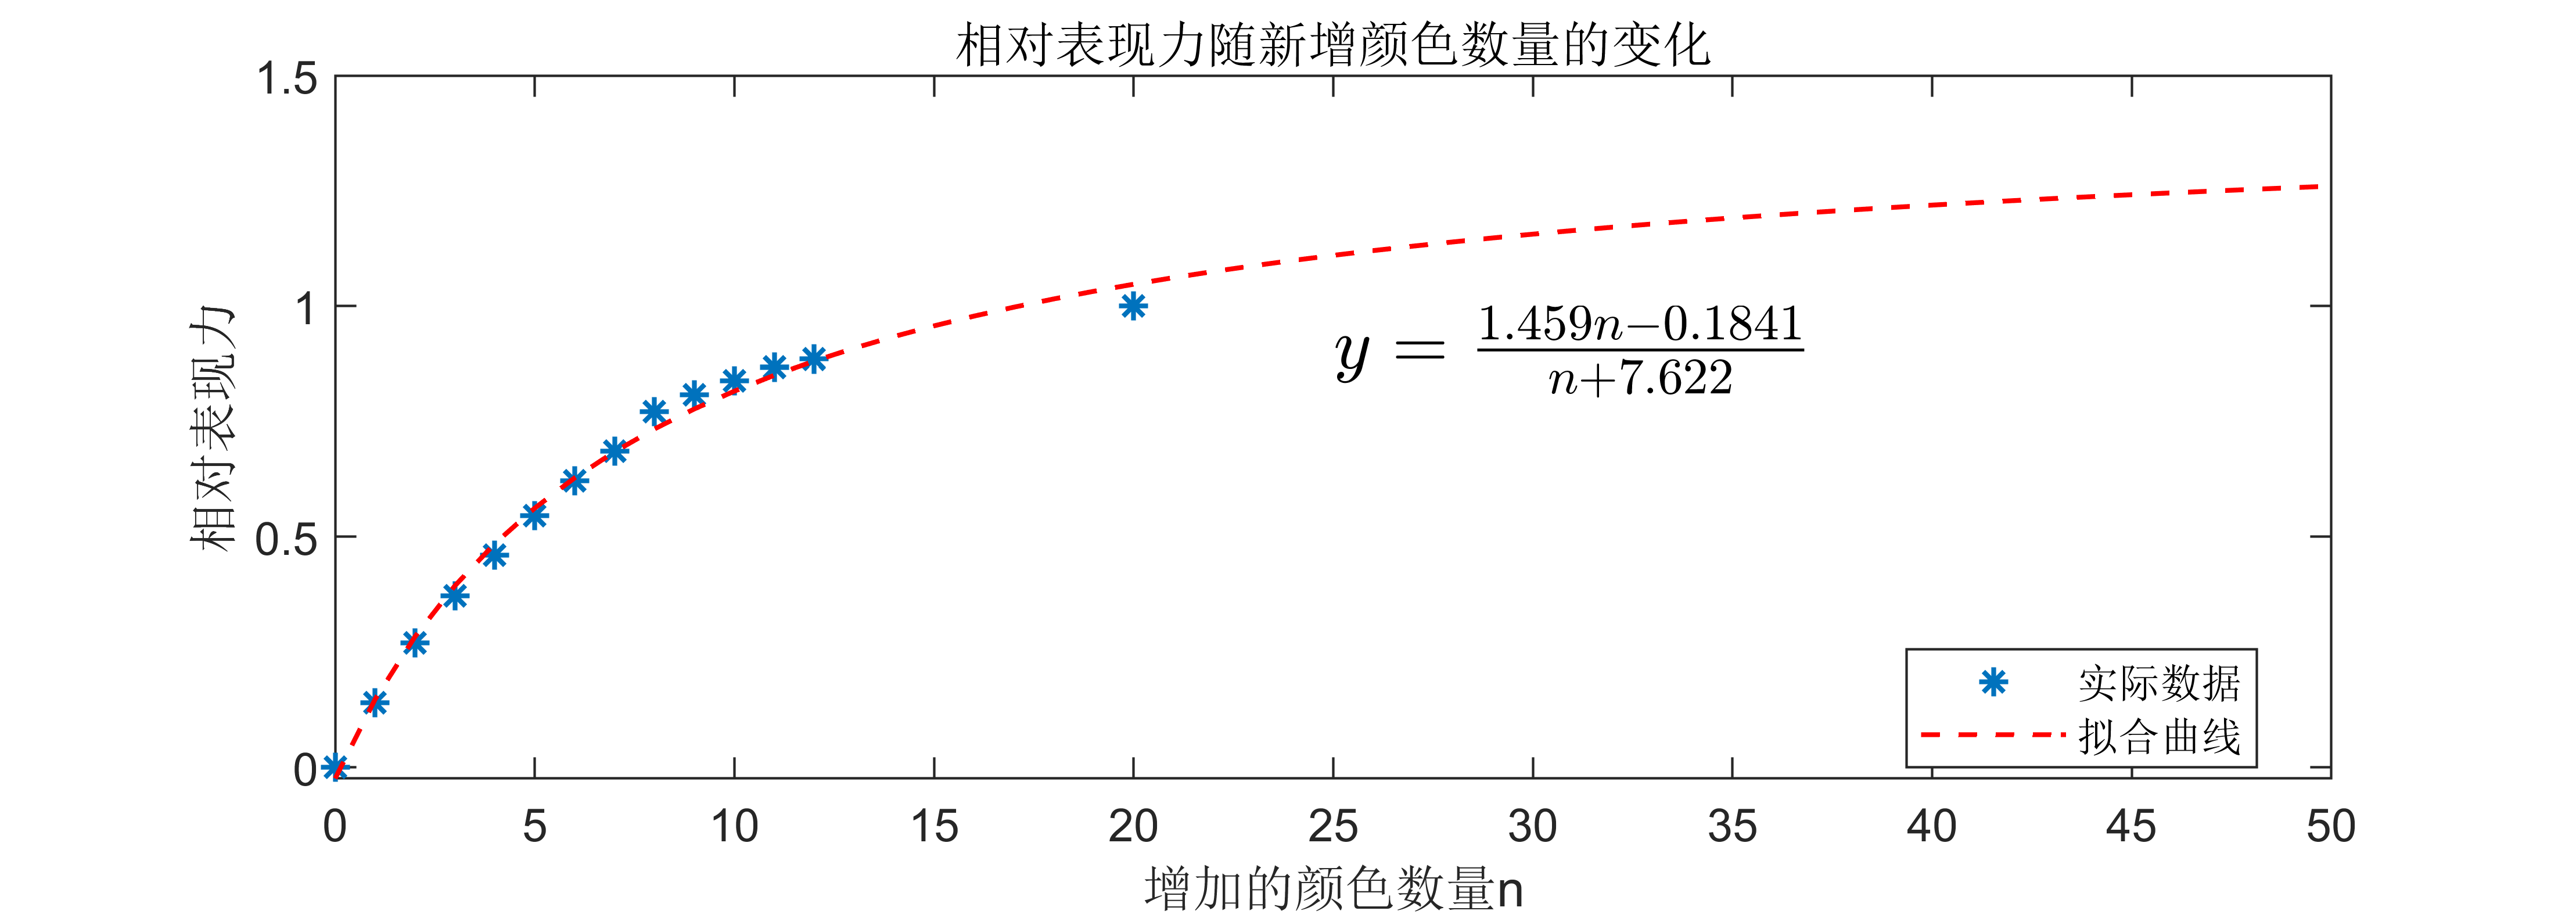
\includegraphics[width=0.85\textwidth]{img/相对表现力随新增颜色数量的变化.png}
 	\caption{相对表现力随新增颜色数量的变化}
 	\label{相对表现力随新增颜色数量的变化}
 \end{figure}
 \subsection{遗传算法求解多目标规划}
 研发一种新颜色瓷砖的成本是相同的,与颜色本身无关,综合考虑成
 本和表现效果,就是建立多目标规划:
 \begin{equation}
 \left\{\begin{array}{ll}
 \min & k n \\
 \max & f(n) .\\
 \text{其中}n > 0
 \end{array}\right.
 \label{dmb}
 \end{equation}
 使用遗传算法求解该多目标规划问题,得到Pareto解集
     \begin{figure}[H]
 	\centering
 	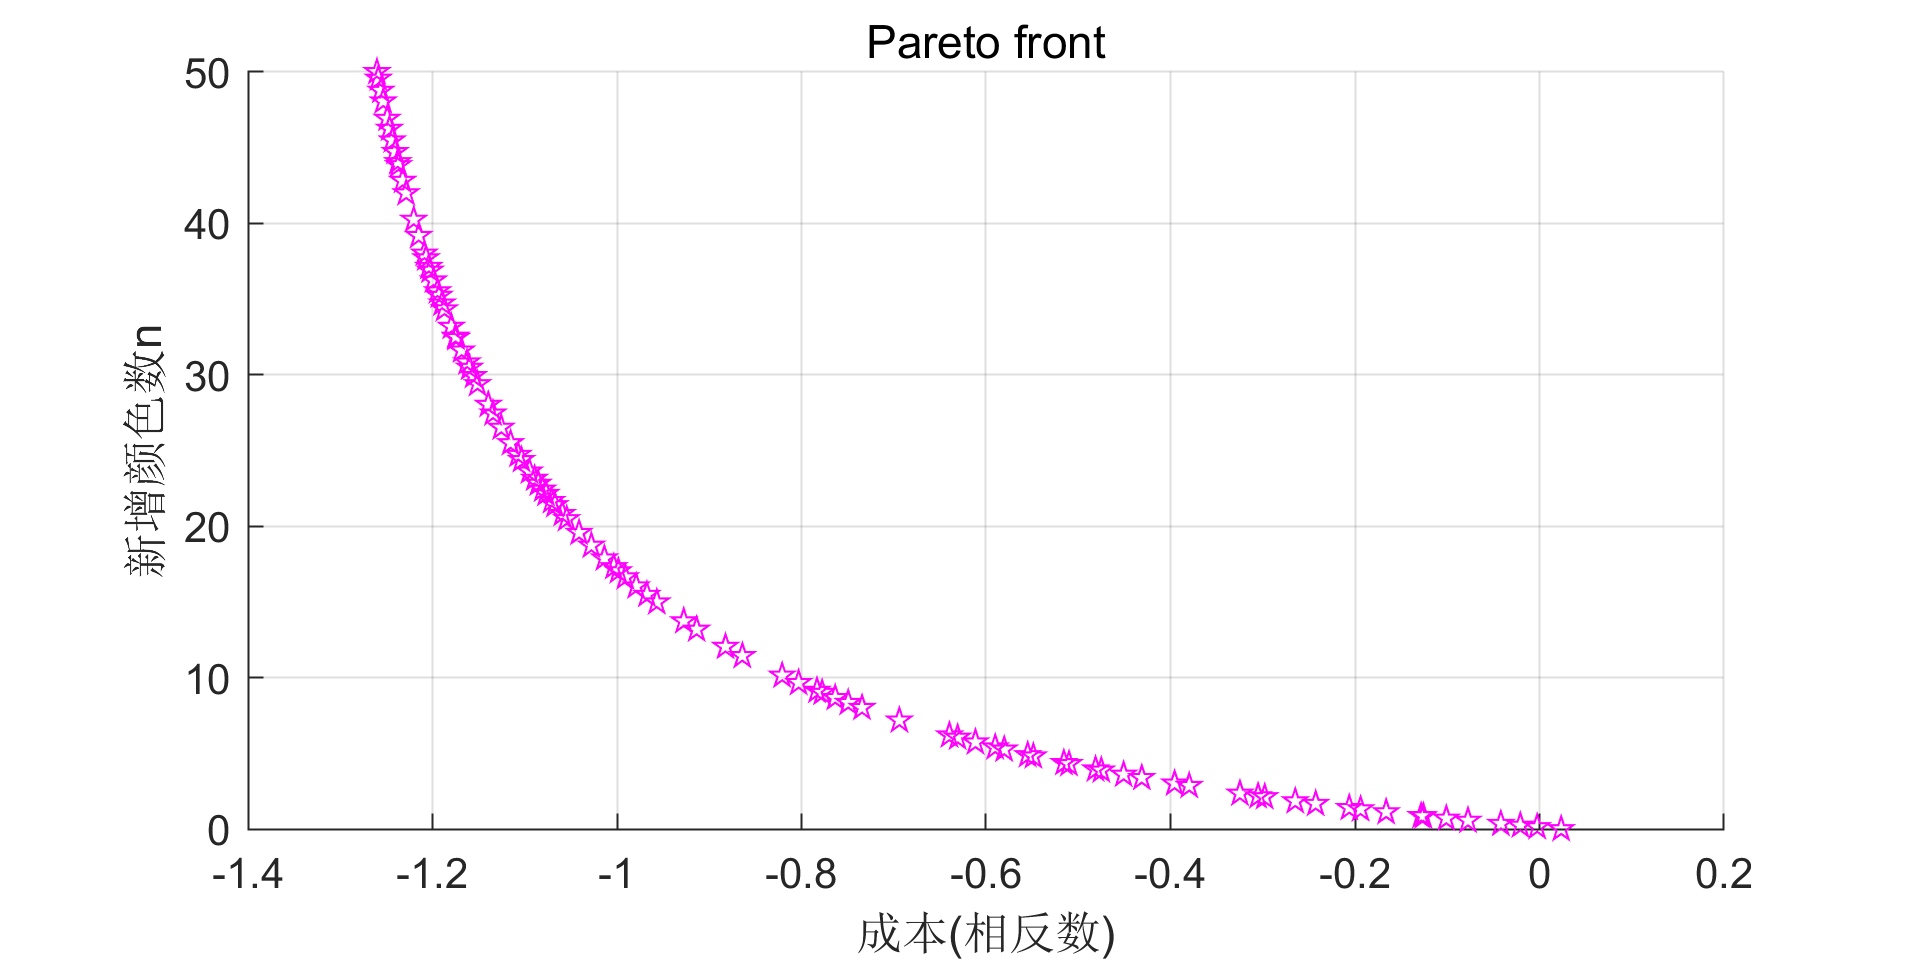
\includegraphics[width=0.7\textwidth]{img/遗传算法多目标规划结果.png}
 	\caption{遗传算法多目标规划结果(Pareto解集)}
 	\label{遗传算法多目标规划结果}
 \end{figure}
可见,我们得到了一系列非劣解,但无法确定最佳解。
 \subsection{熵权法确定评价权重}
 为确定最佳解,使用熵权法确定成本和表现力的权重,进而转化为单目标规划问题。
 
 熵权法是一种客观赋权法,因为它仅依赖于数据本身的离散性。
 对 $n$ 个样本, $m$ 个指标, 则 $x_{i j}$ 为第 $i$ 个样本的第 $j$ 个指标的数值 $i=1, \cdots, n ; j=1, \cdots, m)$
 确定各指标的权重步骤如下:
 1.指标的归一化
 对于正向指标
 \begin{equation}
 x_{i j}^{\prime}=\frac{x_{i j}-\min \left\{x_{1 j}, \ldots, x_{n j}\right\}}{\max \left\{x_{1 j}, \ldots, x_{n j}\right\}-\min \left\{x_{1 j}, \ldots, x_{n j}\right\}}
 \label{zxzb}
 \end{equation}
 对于负向指标
 \begin{equation}
 x_{i j}^{\prime}=\frac{\max \left\{x_{1 j}, \ldots, x_{n j}\right\}-x_{i j}}{\max \left\{x_{1 j}, \ldots, x_{n j}\right\}-\min \left\{x_{1 j}, \ldots, x_{n j}\right\}}
 \end{equation}
 2. 计算第 $j$ 项指标下第 $i$ 个样本值占该指标的比重:
 $$p_{i j}=\frac{x_{i j}}{\sum_{i=1}^{n} x_{i j}}, \quad i=1, \cdots, n, j=1, \cdots, m$$
 3. 计算第 $j$ 项指标的熵值:
 $$e_{j}=-k \sum_{i=1}^{n} p_{i j} \ln \left(p_{i j}\right), \quad j=1, \cdots, m$$
 4. 计算信息熵冗余度 (差异)
 $$d_{j}=1-e_{j}, \quad j=1, \cdots, m$$
 5. 计算各项指标的权重:
 $$w_{j}=\frac{d_{j}}{\sum_{j=1}^{m} d_{j}}, \quad j=1, \cdots, m$$
 
 成本指标与新增颜色数量成正比,设新增颜色数量为1~maxnum(以1为起点,maxnum为终点,间隔为1),因此成本数据也为1~maxnum,表现力数据以新增颜色数量为自变量代入拟合公式\ref{相对表现力随新增颜色数量的变化}求得。对两组数据归一化,计算2个指标的权重。
 \subsection{单目标问题的求解}
 假设求得的权重分别为$q_1,q_2$,则多目标规划问题(公式\eqref{dmb})转换为单目标规划:
  \begin{equation}
 max \quad F(n) = -q_1  GY(n) +q_2 GY(f(n))
 \label{dan}
 \end{equation}
 其中GY为归一化函数\eqref{zxzb}。注意,输入归一化函数GY的自变量为向量,F(n)为数组,即公式中的n不是单个n值,而是$1 \sim n$的数组,计算结果F(n)也为数组。实际上,我们需要找到函数F(n)的最大值对应的横坐标,即为最佳新增颜色数量。
 \subsection{求解结果}
 设置不同的新增颜色数量maxnum,使用熵权法确定权重,当maxnum为20时,权重分别为$0.6444   ,0.3556$,绘制函数\eqref{dan}的图像如图\ref{得分随新增颜色数量的变化}所示,函数值即当前新增颜色数量的相对得分:
      \begin{figure}[H]
 	\centering
 	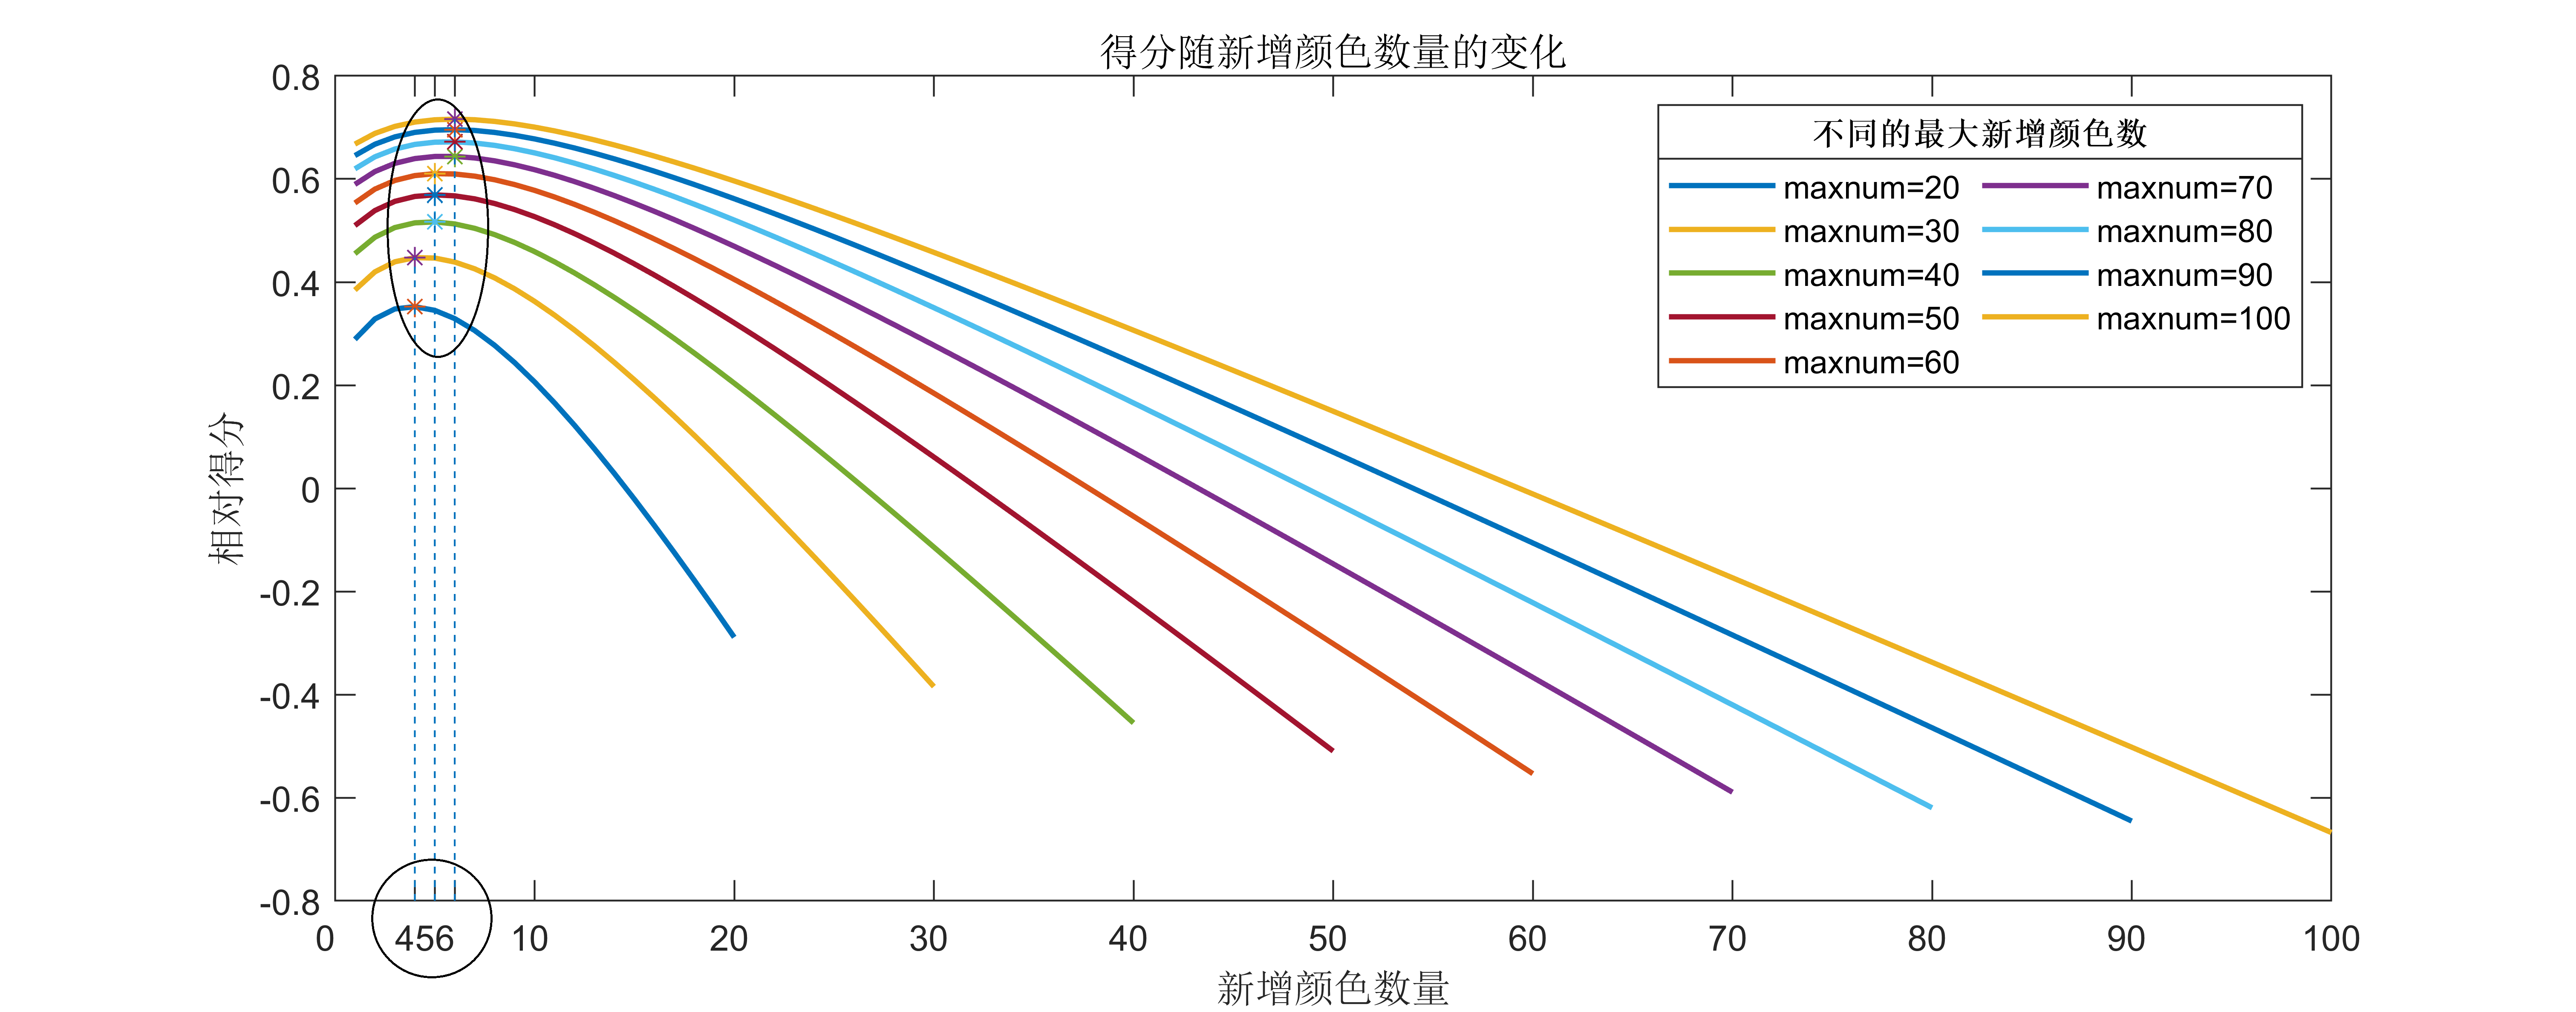
\includegraphics[width=0.9\textwidth]{img/得分随新增颜色数量的变化.png}
 	\caption{得分随新增颜色数量的变化}
 	\label{得分随新增颜色数量的变化}
\end{figure}	
 由图可见,各条曲线最大得分对应的新增颜色数量为4,5,6,因此可以取最佳值为6.即新增颜色数量为6时,得分最高,可以兼顾成本和颜色的表现力。由问题2,新增颜色数量为5时,对应的RGB值如表\ref{6ys},观察表\ref{6ys}最右侧的颜色列,可以看到颜色分布较均匀,没有出现拥挤的现象。
 \begin{table}[H]
 	\centering
 	\caption{新增颜色数量为6时对应的RGB值}
 	\begin{tabularx}{0.9\textwidth}{@{}c *4{>{\centering\arraybackslash}X}@{}}
  		\toprule[1.5pt]
		\textbf{序号} & \textbf{R} & \textbf{G} & \textbf{B} & \textbf{颜色} \\
		\midrule
		\textbf{1} & \textbf{132} & \textbf{0} & \textbf{255} & \cellcolor[rgb]{ .518,  0,  1} \\
		\textbf{2} & \textbf{0} & \textbf{255} & \textbf{10} & \cellcolor[rgb]{ 0,  1,  .039} \\
		\textbf{3} & \textbf{0} & \textbf{0} & \textbf{246} & \cellcolor[rgb]{ 0,  0,  .965} \\
		\textbf{4} & \textbf{113} & \textbf{134} & \textbf{255} & \cellcolor[rgb]{ .443,  .525,  1} \\
		\textbf{5} & \textbf{255} & \textbf{47} & \textbf{251} & \cellcolor[rgb]{ 1,  .184,  .984} \\
		\textbf{6} & \textbf{103} & \textbf{250} & \textbf{152} & \cellcolor[rgb]{ .404,  .98,  .596} \\
		\bottomrule[1.5pt]
 	\end{tabularx}%
 	\label{6ys}%
 \end{table}%
在RGB和LAB颜色空间中绘制新增的颜色点:
      \begin{figure}[H]
	\centering
	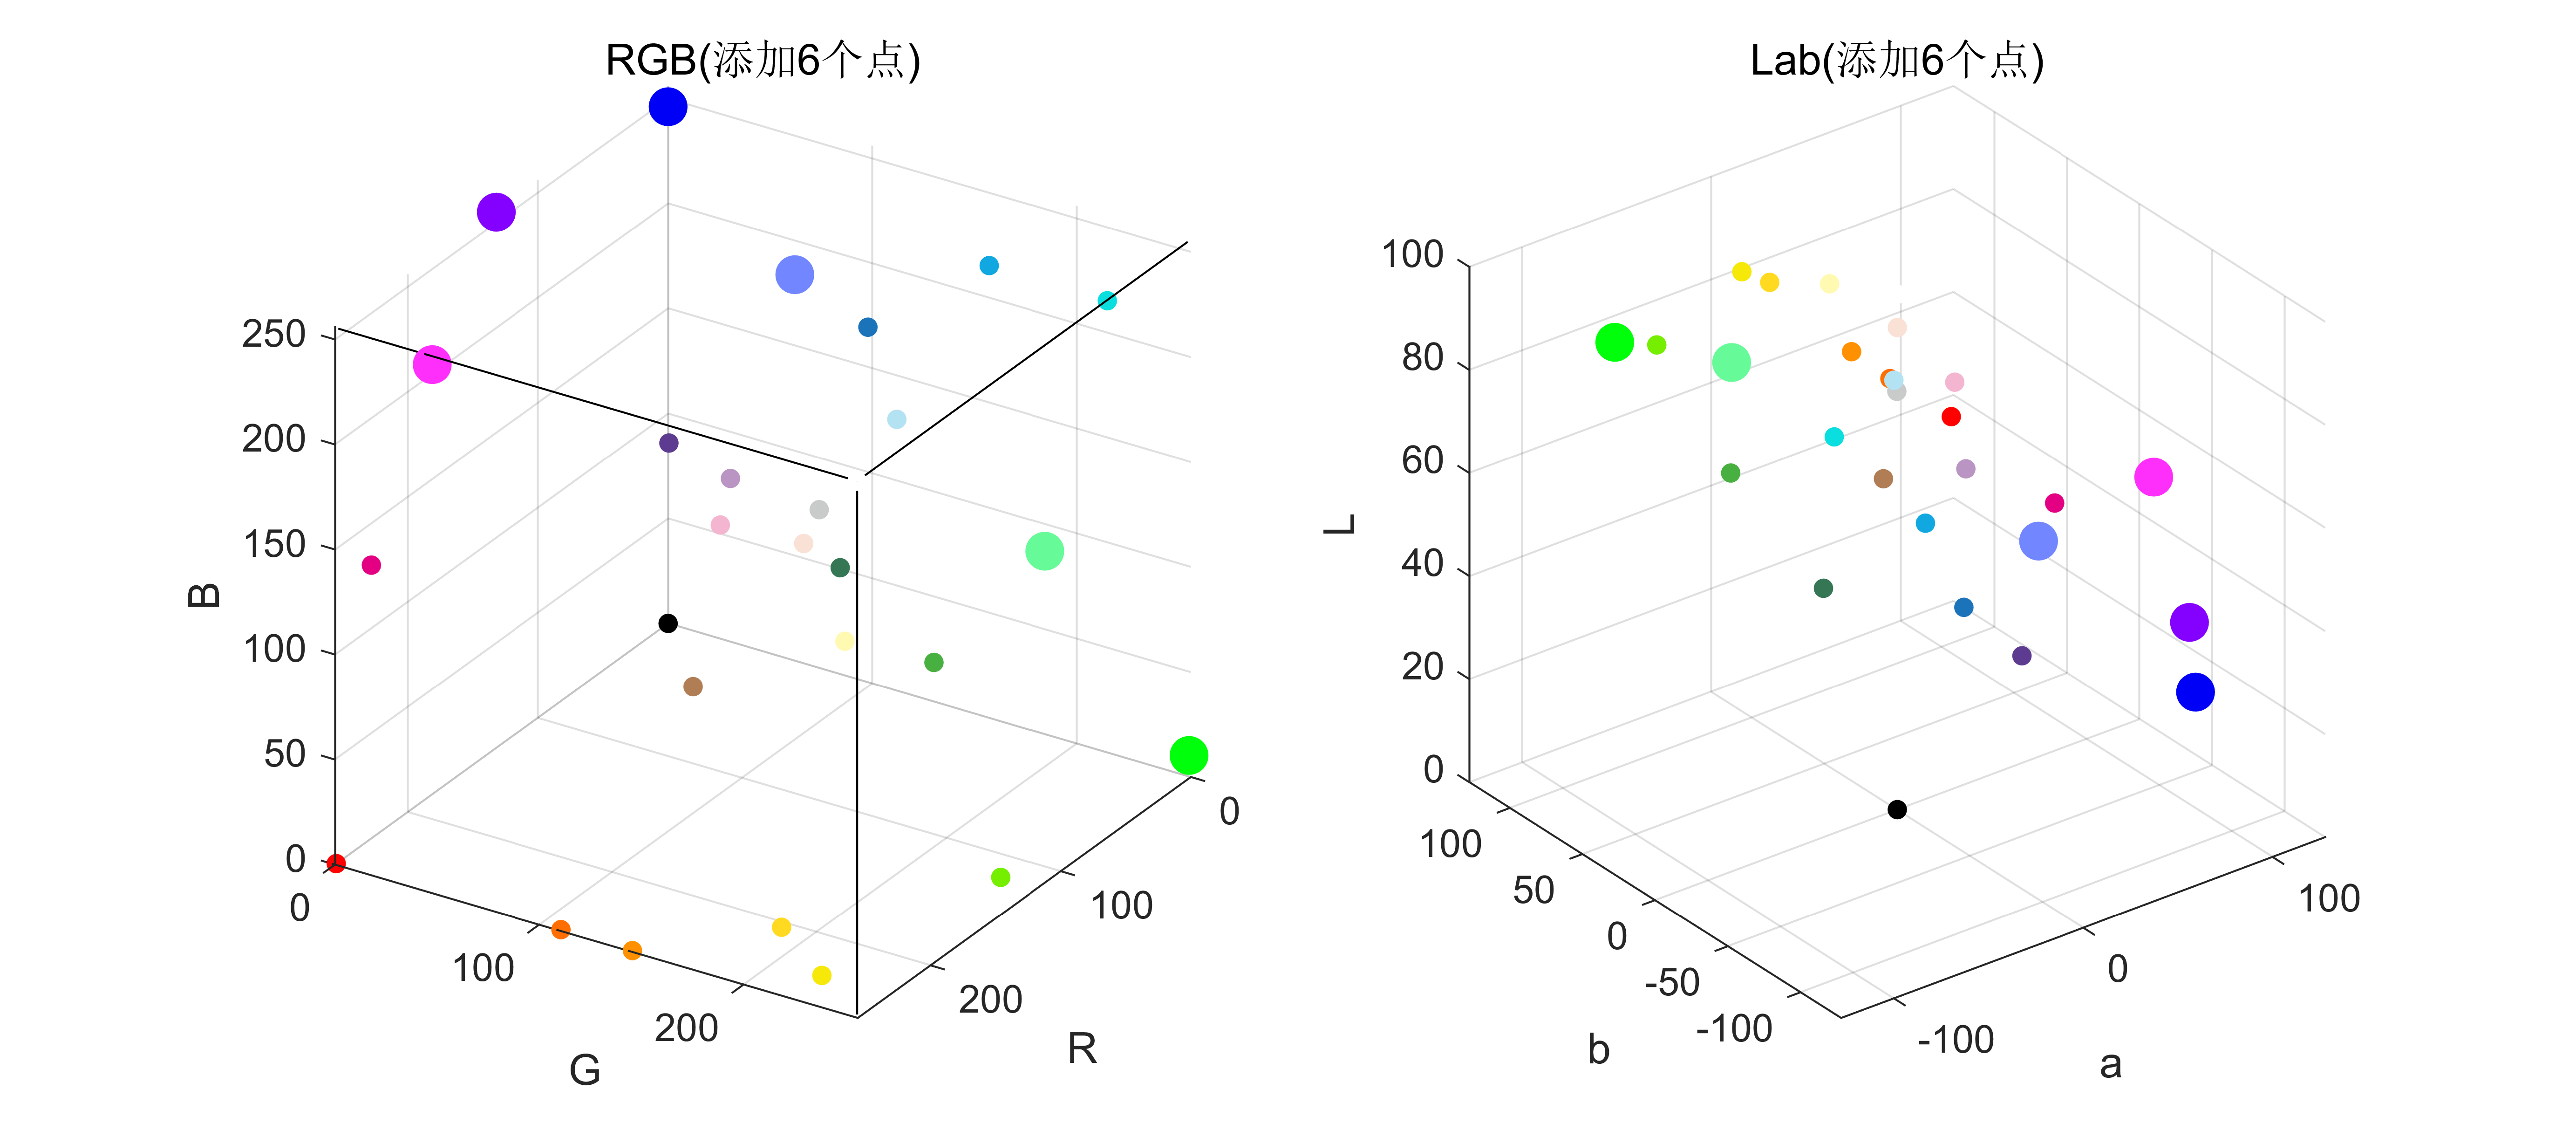
\includegraphics[width=0.95\textwidth]{img/添加6个点.png}
	\caption{新增的6个点在RGB和LAB颜色空间中的分布}
	\label{添加5个点}
\end{figure}
 
 
 \section{模型的评价}
 \subsection{模型的优点}
 \begin{itemize}
 	\item 模型建立在LAB空间上,求解结果能够较好的反映人眼对颜色的感知特点;
 	\item 用颜色点集均匀度量化表现力,较好地处理了问题;
 	\item 整数规划迭代次数很大,确保求得的解尽可能接近最优;
 	\item 找到了表达表现力与新增颜色数量的较精确的函数方程,为进一步的求解作铺垫。
 \end{itemize}
 \subsection{模型的缺点}
  \begin{itemize}
 	\item 问题2中的整数规划问题复杂度较大,使用直接求解法耗时较长,可考虑使用遗传算法等启发式算法优化,减少求解时间。
 \end{itemize}
%\subsection{模型的推广}

 
 
    
    

    
 \section{参考文献}
	%\addcontentsline{toc}{section}{参考文献}
	%\bibliographystyle{gbt7714-2005}
	%\bibliographystyle{gbt7714-numerical}
	\bibliographystyle{unsrt}
	\bibliography{bib/ref}
    
    
 \section{附录}   
 \subsection{问题一相似颜色的对应关系}
 % \begin{table}[H]
% 	\centering
% 	\caption{图像2与给定颜色的对应关系(DE2000)}
% 	\resizebox{\textwidth}{5cm}{
% 	
% 		
%\end{tabular}}%
% \label{tab:addlabel}%
%\end{table}%
 \begin{table}[H]
	\centering
	\caption{图像1与给定颜色的对应关系(DE76)}
	\resizebox{\textwidth}{5cm}{
		    \begin{tabular}{ccccccccccccccccccccccccccc}
			\toprule
			\textbf{1} & \textbf{2} & \textbf{3} & \textbf{4} & \textbf{5} & \textbf{6} & \textbf{7} & \textbf{8} & \textbf{9} & \textbf{10} & \textbf{11} & \textbf{12} & \textbf{13} & \textbf{14} & \textbf{15} & \textbf{16} & \textbf{17} & \textbf{18} & \textbf{19} & \textbf{20} & \textbf{21} & \textbf{22} & \textbf{23} & \textbf{24} & \textbf{25} & \textbf{26} & \textbf{27} \\
			\textbf{1} & \textbf{11} & \textbf{11} & \textbf{11} & \textbf{11} & \textbf{11} & \textbf{7} & \textbf{1} & \textbf{6} & \textbf{11} & \textbf{11} & \textbf{11} & \textbf{7} & \textbf{7} & \textbf{16} & \textbf{6} & \textbf{6} & \textbf{11} & \textbf{5} & \textbf{5} & \textbf{7} & \textbf{16} & \textbf{16} & \textbf{6} & \textbf{5} & \textbf{5} & \textbf{5} \\
			\midrule
			\textbf{28} & \textbf{29} & \textbf{30} & \textbf{31} & \textbf{32} & \textbf{33} & \textbf{34} & \textbf{35} & \textbf{36} & \textbf{37} & \textbf{38} & \textbf{39} & \textbf{40} & \textbf{41} & \textbf{42} & \textbf{43} & \textbf{44} & \textbf{45} & \textbf{46} & \textbf{47} & \textbf{48} & \textbf{49} & \textbf{50} & \textbf{51} & \textbf{52} & \textbf{53} & \textbf{54} \\
			\textbf{12} & \textbf{12} & \textbf{16} & \textbf{15} & \textbf{15} & \textbf{5} & \textbf{5} & \textbf{12} & \textbf{12} & \textbf{1} & \textbf{11} & \textbf{11} & \textbf{11} & \textbf{11} & \textbf{11} & \textbf{7} & \textbf{1} & \textbf{11} & \textbf{11} & \textbf{11} & \textbf{11} & \textbf{7} & \textbf{7} & \textbf{6} & \textbf{6} & \textbf{6} & \textbf{11} \\
			\midrule
			\textbf{55} & \textbf{56} & \textbf{57} & \textbf{58} & \textbf{59} & \textbf{60} & \textbf{61} & \textbf{62} & \textbf{63} & \textbf{64} & \textbf{65} & \textbf{66} & \textbf{67} & \textbf{68} & \textbf{69} & \textbf{70} & \textbf{71} & \textbf{72} & \textbf{73} & \textbf{74} & \textbf{75} & \textbf{76} & \textbf{77} & \textbf{78} & \textbf{79} & \textbf{80} & \textbf{81} \\
			\textbf{5} & \textbf{5} & \textbf{7} & \textbf{16} & \textbf{16} & \textbf{6} & \textbf{5} & \textbf{5} & \textbf{5} & \textbf{12} & \textbf{12} & \textbf{16} & \textbf{15} & \textbf{15} & \textbf{5} & \textbf{5} & \textbf{12} & \textbf{12} & \textbf{1} & \textbf{11} & \textbf{11} & \textbf{11} & \textbf{11} & \textbf{11} & \textbf{10} & \textbf{1} & \textbf{11} \\
			\midrule
			\textbf{82} & \textbf{83} & \textbf{84} & \textbf{85} & \textbf{86} & \textbf{87} & \textbf{88} & \textbf{89} & \textbf{90} & \textbf{91} & \textbf{92} & \textbf{93} & \textbf{94} & \textbf{95} & \textbf{96} & \textbf{97} & \textbf{98} & \textbf{99} & \textbf{100} & \textbf{101} & \textbf{102} & \textbf{103} & \textbf{104} & \textbf{105} & \textbf{106} & \textbf{107} & \textbf{108} \\
			\textbf{11} & \textbf{11} & \textbf{11} & \textbf{7} & \textbf{7} & \textbf{6} & \textbf{6} & \textbf{11} & \textbf{11} & \textbf{5} & \textbf{7} & \textbf{7} & \textbf{16} & \textbf{16} & \textbf{6} & \textbf{5} & \textbf{5} & \textbf{5} & \textbf{12} & \textbf{12} & \textbf{16} & \textbf{15} & \textbf{15} & \textbf{5} & \textbf{5} & \textbf{12} & \textbf{12} \\
			\midrule
			\textbf{109} & \textbf{110} & \textbf{111} & \textbf{112} & \textbf{113} & \textbf{114} & \textbf{115} & \textbf{116} & \textbf{117} & \textbf{118} & \textbf{119} & \textbf{120} & \textbf{121} & \textbf{122} & \textbf{123} & \textbf{124} & \textbf{125} & \textbf{126} & \textbf{127} & \textbf{128} & \textbf{129} & \textbf{130} & \textbf{131} & \textbf{132} & \textbf{133} & \textbf{134} & \textbf{135} \\
			\textbf{10} & \textbf{13} & \textbf{11} & \textbf{11} & \textbf{11} & \textbf{11} & \textbf{10} & \textbf{22} & \textbf{11} & \textbf{11} & \textbf{11} & \textbf{11} & \textbf{10} & \textbf{10} & \textbf{22} & \textbf{22} & \textbf{11} & \textbf{11} & \textbf{5} & \textbf{7} & \textbf{7} & \textbf{18} & \textbf{6} & \textbf{6} & \textbf{5} & \textbf{5} & \textbf{5} \\
			\midrule
			\textbf{136} & \textbf{137} & \textbf{138} & \textbf{139} & \textbf{140} & \textbf{141} & \textbf{142} & \textbf{143} & \textbf{144} & \textbf{145} & \textbf{146} & \textbf{147} & \textbf{148} & \textbf{149} & \textbf{150} & \textbf{151} & \textbf{152} & \textbf{153} & \textbf{154} & \textbf{155} & \textbf{156} & \textbf{157} & \textbf{158} & \textbf{159} & \textbf{160} & \textbf{161} & \textbf{162} \\
			\textbf{12} & \textbf{20} & \textbf{16} & \textbf{15} & \textbf{15} & \textbf{5} & \textbf{5} & \textbf{12} & \textbf{20} & \textbf{13} & \textbf{13} & \textbf{13} & \textbf{11} & \textbf{11} & \textbf{11} & \textbf{10} & \textbf{10} & \textbf{13} & \textbf{11} & \textbf{11} & \textbf{11} & \textbf{10} & \textbf{10} & \textbf{22} & \textbf{22} & \textbf{11} & \textbf{11} \\
			\midrule
			\textbf{163} & \textbf{164} & \textbf{165} & \textbf{166} & \textbf{167} & \textbf{168} & \textbf{169} & \textbf{170} & \textbf{171} & \textbf{172} & \textbf{173} & \textbf{174} & \textbf{175} & \textbf{176} & \textbf{177} & \textbf{178} & \textbf{179} & \textbf{180} & \textbf{181} & \textbf{182} & \textbf{183} & \textbf{184} & \textbf{185} & \textbf{186} & \textbf{187} & \textbf{188} & \textbf{189} \\
			\textbf{10} & \textbf{10} & \textbf{10} & \textbf{22} & \textbf{22} & \textbf{22} & \textbf{4} & \textbf{5} & \textbf{19} & \textbf{18} & \textbf{18} & \textbf{22} & \textbf{15} & \textbf{15} & \textbf{5} & \textbf{19} & \textbf{20} & \textbf{20} & \textbf{3} & \textbf{13} & \textbf{13} & \textbf{13} & \textbf{13} & \textbf{13} & \textbf{17} & \textbf{13} & \textbf{13} \\
			\midrule
			\textbf{190} & \textbf{191} & \textbf{192} & \textbf{193} & \textbf{194} & \textbf{195} & \textbf{196} & \textbf{197} & \textbf{198} & \textbf{199} & \textbf{200} & \textbf{201} & \textbf{202} & \textbf{203} & \textbf{204} & \textbf{205} & \textbf{206} & \textbf{207} & \textbf{208} & \textbf{209} & \textbf{210} & \textbf{211} & \textbf{212} & \textbf{213} & \textbf{214} & \textbf{215} & \textbf{216} \\
			\textbf{13} & \textbf{13} & \textbf{11} & \textbf{17} & \textbf{10} & \textbf{8} & \textbf{22} & \textbf{11} & \textbf{11} & \textbf{9} & \textbf{10} & \textbf{10} & \textbf{8} & \textbf{22} & \textbf{22} & \textbf{14} & \textbf{14} & \textbf{19} & \textbf{21} & \textbf{18} & \textbf{22} & \textbf{4} & \textbf{4} & \textbf{19} & \textbf{19} & \textbf{2} & \textbf{20} \\
			\bottomrule
		\end{tabular}}%
	\label{tab:addlabel}%
\end{table}%

 \begin{table}[H]
	\centering
	\caption{图像2与给定颜色的对应关系(DE76)}
	\resizebox{\textwidth}{5cm}{
		
	    \begin{tabular}{ccccccccccccccccccccccccc}
		\toprule
		\textbf{1} & \textbf{2} & \textbf{3} & \textbf{4} & \textbf{5} & \textbf{6} & \textbf{7} & \textbf{8} & \textbf{9} & \textbf{10} & \textbf{11} & \textbf{12} & \textbf{13} & \textbf{14} & \textbf{15} & \textbf{16} & \textbf{17} & \textbf{18} & \textbf{19} & \textbf{20} & \textbf{21} & \textbf{22} & \textbf{23} & \textbf{24} & \textbf{25} \\
		\textbf{12} & \textbf{5} & \textbf{6} & \textbf{6} & \textbf{5} & \textbf{12} & \textbf{11} & \textbf{7} & \textbf{6} & \textbf{6} & \textbf{11} & \textbf{7} & \textbf{16} & \textbf{5} & \textbf{6} & \textbf{5} & \textbf{12} & \textbf{5} & \textbf{12} & \textbf{5} & \textbf{11} & \textbf{7} & \textbf{5} & \textbf{7} & \textbf{16} \\
		\midrule
		\textbf{26} & \textbf{27} & \textbf{28} & \textbf{29} & \textbf{30} & \textbf{31} & \textbf{32} & \textbf{33} & \textbf{34} & \textbf{35} & \textbf{36} & \textbf{37} & \textbf{38} & \textbf{39} & \textbf{40} & \textbf{41} & \textbf{42} & \textbf{43} & \textbf{44} & \textbf{45} & \textbf{46} & \textbf{47} & \textbf{48} & \textbf{49} & \textbf{50} \\
		\textbf{5} & \textbf{11} & \textbf{6} & \textbf{6} & \textbf{5} & \textbf{12} & \textbf{5} & \textbf{11} & \textbf{7} & \textbf{7} & \textbf{5} & \textbf{12} & \textbf{12} & \textbf{11} & \textbf{7} & \textbf{7} & \textbf{15} & \textbf{5} & \textbf{11} & \textbf{6} & \textbf{1} & \textbf{7} & \textbf{11} & \textbf{11} & \textbf{6} \\
		\midrule
		\textbf{51} & \textbf{52} & \textbf{53} & \textbf{54} & \textbf{55} & \textbf{56} & \textbf{57} & \textbf{58} & \textbf{59} & \textbf{60} & \textbf{61} & \textbf{62} & \textbf{63} & \textbf{64} & \textbf{65} & \textbf{66} & \textbf{67} & \textbf{68} & \textbf{69} & \textbf{70} & \textbf{71} & \textbf{72} & \textbf{73} & \textbf{74} & \textbf{75} \\
		\textbf{6} & \textbf{16} & \textbf{16} & \textbf{11} & \textbf{11} & \textbf{7} & \textbf{11} & \textbf{16} & \textbf{11} & \textbf{11} & \textbf{6} & \textbf{15} & \textbf{6} & \textbf{12} & \textbf{11} & \textbf{5} & \textbf{12} & \textbf{7} & \textbf{5} & \textbf{12} & \textbf{1} & \textbf{11} & \textbf{5} & \textbf{11} & \textbf{6} \\
		\midrule
		\textbf{76} & \textbf{77} & \textbf{78} & \textbf{79} & \textbf{80} & \textbf{81} & \textbf{82} & \textbf{83} & \textbf{84} & \textbf{85} & \textbf{86} & \textbf{87} & \textbf{88} & \textbf{89} & \textbf{90} & \textbf{91} & \textbf{92} & \textbf{93} & \textbf{94} & \textbf{95} & \textbf{96} & \textbf{97} & \textbf{98} & \textbf{99} & \textbf{100} \\
		\textbf{11} & \textbf{7} & \textbf{16} & \textbf{1} & \textbf{11} & \textbf{11} & \textbf{6} & \textbf{12} & \textbf{7} & \textbf{5} & \textbf{7} & \textbf{11} & \textbf{11} & \textbf{16} & \textbf{12} & \textbf{5} & \textbf{11} & \textbf{11} & \textbf{10} & \textbf{11} & \textbf{5} & \textbf{11} & \textbf{5} & \textbf{6} & \textbf{7} \\
		\midrule
		\textbf{101} & \textbf{102} & \textbf{103} & \textbf{104} & \textbf{105} & \textbf{106} & \textbf{107} & \textbf{108} & \textbf{109} & \textbf{110} & \textbf{111} & \textbf{112} & \textbf{113} & \textbf{114} & \textbf{115} & \textbf{116} & \textbf{117} & \textbf{118} & \textbf{119} & \textbf{120} & \textbf{121} & \textbf{122} & \textbf{123} & \textbf{124} & \textbf{125} \\
		\textbf{11} & \textbf{11} & \textbf{5} & \textbf{5} & \textbf{11} & \textbf{11} & \textbf{10} & \textbf{10} & \textbf{10} & \textbf{15} & \textbf{5} & \textbf{20} & \textbf{10} & \textbf{20} & \textbf{7} & \textbf{11} & \textbf{10} & \textbf{20} & \textbf{13} & \textbf{12} & \textbf{15} & \textbf{5} & \textbf{13} & \textbf{11} & \textbf{20} \\
		\midrule
		\textbf{126} & \textbf{127} & \textbf{128} & \textbf{129} & \textbf{130} & \textbf{131} & \textbf{132} & \textbf{133} & \textbf{134} & \textbf{135} & \textbf{136} & \textbf{137} & \textbf{138} & \textbf{139} & \textbf{140} & \textbf{141} & \textbf{142} & \textbf{143} & \textbf{144} & \textbf{145} & \textbf{146} & \textbf{147} & \textbf{148} & \textbf{149} & \textbf{150} \\
		\textbf{5} & \textbf{18} & \textbf{11} & \textbf{10} & \textbf{10} & \textbf{14} & \textbf{22} & \textbf{11} & \textbf{11} & \textbf{10} & \textbf{10} & \textbf{13} & \textbf{22} & \textbf{3} & \textbf{22} & \textbf{9} & \textbf{18} & \textbf{5} & \textbf{10} & \textbf{20} & \textbf{13} & \textbf{22} & \textbf{22} & \textbf{18} & \textbf{19} \\
		\midrule
		\textbf{151} & \textbf{152} & \textbf{153} & \textbf{154} & \textbf{155} & \textbf{156} & \textbf{157} & \textbf{158} & \textbf{159} & \textbf{160} & \textbf{161} & \textbf{162} & \textbf{163} & \textbf{164} & \textbf{165} & \textbf{166} & \textbf{167} & \textbf{168} & \textbf{169} & \textbf{170} & \textbf{171} & \textbf{172} & \textbf{173} & \textbf{174} & \textbf{175} \\
		\textbf{10} & \textbf{14} & \textbf{13} & \textbf{17} & \textbf{10} & \textbf{19} & \textbf{11} & \textbf{19} & \textbf{10} & \textbf{13} & \textbf{18} & \textbf{3} & \textbf{13} & \textbf{11} & \textbf{13} & \textbf{9} & \textbf{13} & \textbf{10} & \textbf{10} & \textbf{11} & \textbf{13} & \textbf{17} & \textbf{22} & \textbf{4} & \textbf{8} \\
		\midrule
		\textbf{176} & \textbf{177} & \textbf{178} & \textbf{179} & \textbf{180} & \textbf{181} & \textbf{182} & \textbf{183} & \textbf{184} & \textbf{185} & \textbf{186} & \textbf{187} & \textbf{188} & \textbf{189} & \textbf{190} & \textbf{191} & \textbf{192} & \textbf{193} & \textbf{194} & \textbf{195} & \textbf{196} & \textbf{197} & \textbf{198} & \textbf{199} & \textbf{200} \\
		\textbf{19} & \textbf{19} & \textbf{19} & \textbf{13} & \textbf{8} & \textbf{2} & \textbf{13} & \textbf{10} & \textbf{19} & \textbf{22} & \textbf{14} & \textbf{8} & \textbf{13} & \textbf{14} & \textbf{4} & \textbf{22} & \textbf{10} & \textbf{17} & \textbf{17} & \textbf{4} & \textbf{8} & \textbf{8} & \textbf{13} & \textbf{13} & \textbf{9} \\
		\bottomrule	
\end{tabular}}%
\label{tab:addlabel}%
\end{table}%



 \begin{table}[H]
 	\centering
 	\caption{图像1与给定颜色的对应关系(DE2000)}
 	\resizebox{\textwidth}{5cm}{
    \begin{tabular}{ccccccccccccccccccccccccccc}
	\toprule
	\textbf{1} & \textbf{2} & \textbf{3} & \textbf{4} & \textbf{5} & \textbf{6} & \textbf{7} & \textbf{8} & \textbf{9} & \textbf{10} & \textbf{11} & \textbf{12} & \textbf{13} & \textbf{14} & \textbf{15} & \textbf{16} & \textbf{17} & \textbf{18} & \textbf{19} & \textbf{20} & \textbf{21} & \textbf{22} & \textbf{23} & \textbf{24} & \textbf{25} & \textbf{26} & \textbf{27} \\
	\textbf{1} & \textbf{11} & \textbf{11} & \textbf{11} & \textbf{11} & \textbf{11} & \textbf{7} & \textbf{11} & \textbf{11} & \textbf{11} & \textbf{11} & \textbf{11} & \textbf{7} & \textbf{7} & \textbf{6} & \textbf{6} & \textbf{6} & \textbf{6} & \textbf{5} & \textbf{5} & \textbf{7} & \textbf{16} & \textbf{16} & \textbf{16} & \textbf{5} & \textbf{5} & \textbf{5} \\
	\midrule
	\textbf{28} & \textbf{29} & \textbf{30} & \textbf{31} & \textbf{32} & \textbf{33} & \textbf{34} & \textbf{35} & \textbf{36} & \textbf{37} & \textbf{38} & \textbf{39} & \textbf{40} & \textbf{41} & \textbf{42} & \textbf{43} & \textbf{44} & \textbf{45} & \textbf{46} & \textbf{47} & \textbf{48} & \textbf{49} & \textbf{50} & \textbf{51} & \textbf{52} & \textbf{53} & \textbf{54} \\
	\textbf{12} & \textbf{12} & \textbf{16} & \textbf{15} & \textbf{15} & \textbf{15} & \textbf{12} & \textbf{12} & \textbf{12} & \textbf{1} & \textbf{11} & \textbf{11} & \textbf{11} & \textbf{11} & \textbf{11} & \textbf{7} & \textbf{11} & \textbf{11} & \textbf{11} & \textbf{11} & \textbf{11} & \textbf{7} & \textbf{7} & \textbf{6} & \textbf{6} & \textbf{6} & \textbf{6} \\
	\midrule
	\textbf{55} & \textbf{56} & \textbf{57} & \textbf{58} & \textbf{59} & \textbf{60} & \textbf{61} & \textbf{62} & \textbf{63} & \textbf{64} & \textbf{65} & \textbf{66} & \textbf{67} & \textbf{68} & \textbf{69} & \textbf{70} & \textbf{71} & \textbf{72} & \textbf{73} & \textbf{74} & \textbf{75} & \textbf{76} & \textbf{77} & \textbf{78} & \textbf{79} & \textbf{80} & \textbf{81} \\
	\textbf{5} & \textbf{5} & \textbf{7} & \textbf{16} & \textbf{16} & \textbf{16} & \textbf{5} & \textbf{5} & \textbf{5} & \textbf{12} & \textbf{12} & \textbf{16} & \textbf{15} & \textbf{15} & \textbf{15} & \textbf{12} & \textbf{12} & \textbf{12} & \textbf{1} & \textbf{11} & \textbf{11} & \textbf{11} & \textbf{11} & \textbf{11} & \textbf{1} & \textbf{11} & \textbf{11} \\
	\midrule
	\textbf{82} & \textbf{83} & \textbf{84} & \textbf{85} & \textbf{86} & \textbf{87} & \textbf{88} & \textbf{89} & \textbf{90} & \textbf{91} & \textbf{92} & \textbf{93} & \textbf{94} & \textbf{95} & \textbf{96} & \textbf{97} & \textbf{98} & \textbf{99} & \textbf{100} & \textbf{101} & \textbf{102} & \textbf{103} & \textbf{104} & \textbf{105} & \textbf{106} & \textbf{107} & \textbf{108} \\
	\textbf{11} & \textbf{11} & \textbf{11} & \textbf{7} & \textbf{7} & \textbf{6} & \textbf{6} & \textbf{6} & \textbf{6} & \textbf{5} & \textbf{5} & \textbf{7} & \textbf{16} & \textbf{16} & \textbf{16} & \textbf{5} & \textbf{5} & \textbf{5} & \textbf{12} & \textbf{12} & \textbf{16} & \textbf{15} & \textbf{15} & \textbf{15} & \textbf{15} & \textbf{12} & \textbf{12} \\
	\midrule
	\textbf{109} & \textbf{110} & \textbf{111} & \textbf{112} & \textbf{113} & \textbf{114} & \textbf{115} & \textbf{116} & \textbf{117} & \textbf{118} & \textbf{119} & \textbf{120} & \textbf{121} & \textbf{122} & \textbf{123} & \textbf{124} & \textbf{125} & \textbf{126} & \textbf{127} & \textbf{128} & \textbf{129} & \textbf{130} & \textbf{131} & \textbf{132} & \textbf{133} & \textbf{134} & \textbf{135} \\
	\textbf{13} & \textbf{11} & \textbf{11} & \textbf{11} & \textbf{11} & \textbf{11} & \textbf{10} & \textbf{13} & \textbf{11} & \textbf{11} & \textbf{11} & \textbf{11} & \textbf{10} & \textbf{10} & \textbf{22} & \textbf{11} & \textbf{11} & \textbf{6} & \textbf{5} & \textbf{5} & \textbf{7} & \textbf{16} & \textbf{6} & \textbf{6} & \textbf{5} & \textbf{5} & \textbf{5} \\
	\midrule
	\textbf{136} & \textbf{137} & \textbf{138} & \textbf{139} & \textbf{140} & \textbf{141} & \textbf{142} & \textbf{143} & \textbf{144} & \textbf{145} & \textbf{146} & \textbf{147} & \textbf{148} & \textbf{149} & \textbf{150} & \textbf{151} & \textbf{152} & \textbf{153} & \textbf{154} & \textbf{155} & \textbf{156} & \textbf{157} & \textbf{158} & \textbf{159} & \textbf{160} & \textbf{161} & \textbf{162} \\
	\textbf{12} & \textbf{20} & \textbf{16} & \textbf{15} & \textbf{15} & \textbf{15} & \textbf{15} & \textbf{12} & \textbf{20} & \textbf{3} & \textbf{13} & \textbf{13} & \textbf{11} & \textbf{11} & \textbf{11} & \textbf{3} & \textbf{13} & \textbf{13} & \textbf{13} & \textbf{11} & \textbf{11} & \textbf{10} & \textbf{10} & \textbf{13} & \textbf{22} & \textbf{22} & \textbf{22} \\
	\midrule
	\textbf{163} & \textbf{164} & \textbf{165} & \textbf{166} & \textbf{167} & \textbf{168} & \textbf{169} & \textbf{170} & \textbf{171} & \textbf{172} & \textbf{173} & \textbf{174} & \textbf{175} & \textbf{176} & \textbf{177} & \textbf{178} & \textbf{179} & \textbf{180} & \textbf{181} & \textbf{182} & \textbf{183} & \textbf{184} & \textbf{185} & \textbf{186} & \textbf{187} & \textbf{188} & \textbf{189} \\
	\textbf{10} & \textbf{10} & \textbf{10} & \textbf{22} & \textbf{22} & \textbf{22} & \textbf{4} & \textbf{15} & \textbf{5} & \textbf{18} & \textbf{18} & \textbf{20} & \textbf{15} & \textbf{15} & \textbf{15} & \textbf{15} & \textbf{12} & \textbf{20} & \textbf{3} & \textbf{13} & \textbf{13} & \textbf{13} & \textbf{13} & \textbf{13} & \textbf{3} & \textbf{13} & \textbf{13} \\
	\midrule
	\textbf{190} & \textbf{191} & \textbf{192} & \textbf{193} & \textbf{194} & \textbf{195} & \textbf{196} & \textbf{197} & \textbf{198} & \textbf{199} & \textbf{200} & \textbf{201} & \textbf{202} & \textbf{203} & \textbf{204} & \textbf{205} & \textbf{206} & \textbf{207} & \textbf{208} & \textbf{209} & \textbf{210} & \textbf{211} & \textbf{212} & \textbf{213} & \textbf{214} & \textbf{215} & \textbf{216} \\
	\textbf{13} & \textbf{13} & \textbf{22} & \textbf{17} & \textbf{3} & \textbf{13} & \textbf{13} & \textbf{22} & \textbf{22} & \textbf{9} & \textbf{9} & \textbf{10} & \textbf{8} & \textbf{22} & \textbf{22} & \textbf{14} & \textbf{14} & \textbf{19} & \textbf{21} & \textbf{8} & \textbf{22} & \textbf{4} & \textbf{4} & \textbf{19} & \textbf{19} & \textbf{2} & \textbf{20} \\
	\bottomrule
 	\end{tabular}}%
 	\label{tab:addlabel}%
 \end{table}%
 
 \begin{table}[H]
 	\centering
 	\caption{图像2与给定颜色的对应关系(DE2000)}
 	\resizebox{\textwidth}{5cm}{
    \begin{tabular}{ccccccccccccccccccccccccc}
	\toprule
	\textbf{1} & \textbf{2} & \textbf{3} & \textbf{4} & \textbf{5} & \textbf{6} & \textbf{7} & \textbf{8} & \textbf{9} & \textbf{10} & \textbf{11} & \textbf{12} & \textbf{13} & \textbf{14} & \textbf{15} & \textbf{16} & \textbf{17} & \textbf{18} & \textbf{19} & \textbf{20} & \textbf{21} & \textbf{22} & \textbf{23} & \textbf{24} & \textbf{25} \\
	\textbf{12} & \textbf{15} & \textbf{6} & \textbf{6} & \textbf{5} & \textbf{12} & \textbf{11} & \textbf{7} & \textbf{6} & \textbf{16} & \textbf{6} & \textbf{7} & \textbf{16} & \textbf{15} & \textbf{6} & \textbf{5} & \textbf{12} & \textbf{5} & \textbf{5} & \textbf{5} & \textbf{11} & \textbf{7} & \textbf{5} & \textbf{7} & \textbf{16} \\
	\midrule
	\textbf{26} & \textbf{27} & \textbf{28} & \textbf{29} & \textbf{30} & \textbf{31} & \textbf{32} & \textbf{33} & \textbf{34} & \textbf{35} & \textbf{36} & \textbf{37} & \textbf{38} & \textbf{39} & \textbf{40} & \textbf{41} & \textbf{42} & \textbf{43} & \textbf{44} & \textbf{45} & \textbf{46} & \textbf{47} & \textbf{48} & \textbf{49} & \textbf{50} \\
	\textbf{5} & \textbf{11} & \textbf{6} & \textbf{6} & \textbf{5} & \textbf{12} & \textbf{5} & \textbf{11} & \textbf{7} & \textbf{6} & \textbf{5} & \textbf{12} & \textbf{5} & \textbf{11} & \textbf{7} & \textbf{7} & \textbf{15} & \textbf{5} & \textbf{11} & \textbf{11} & \textbf{11} & \textbf{7} & \textbf{11} & \textbf{11} & \textbf{6} \\
	\midrule
	\textbf{51} & \textbf{52} & \textbf{53} & \textbf{54} & \textbf{55} & \textbf{56} & \textbf{57} & \textbf{58} & \textbf{59} & \textbf{60} & \textbf{61} & \textbf{62} & \textbf{63} & \textbf{64} & \textbf{65} & \textbf{66} & \textbf{67} & \textbf{68} & \textbf{69} & \textbf{70} & \textbf{71} & \textbf{72} & \textbf{73} & \textbf{74} & \textbf{75} \\
	\textbf{16} & \textbf{16} & \textbf{16} & \textbf{11} & \textbf{11} & \textbf{7} & \textbf{11} & \textbf{16} & \textbf{11} & \textbf{11} & \textbf{6} & \textbf{15} & \textbf{6} & \textbf{12} & \textbf{6} & \textbf{5} & \textbf{12} & \textbf{7} & \textbf{5} & \textbf{12} & \textbf{1} & \textbf{11} & \textbf{5} & \textbf{11} & \textbf{6} \\
	\midrule
	\textbf{76} & \textbf{77} & \textbf{78} & \textbf{79} & \textbf{80} & \textbf{81} & \textbf{82} & \textbf{83} & \textbf{84} & \textbf{85} & \textbf{86} & \textbf{87} & \textbf{88} & \textbf{89} & \textbf{90} & \textbf{91} & \textbf{92} & \textbf{93} & \textbf{94} & \textbf{95} & \textbf{96} & \textbf{97} & \textbf{98} & \textbf{99} & \textbf{100} \\
	\textbf{11} & \textbf{7} & \textbf{16} & \textbf{11} & \textbf{11} & \textbf{11} & \textbf{11} & \textbf{12} & \textbf{5} & \textbf{15} & \textbf{7} & \textbf{11} & \textbf{11} & \textbf{16} & \textbf{12} & \textbf{5} & \textbf{11} & \textbf{11} & \textbf{10} & \textbf{11} & \textbf{5} & \textbf{11} & \textbf{15} & \textbf{6} & \textbf{5} \\
	\midrule
	\textbf{101} & \textbf{102} & \textbf{103} & \textbf{104} & \textbf{105} & \textbf{106} & \textbf{107} & \textbf{108} & \textbf{109} & \textbf{110} & \textbf{111} & \textbf{112} & \textbf{113} & \textbf{114} & \textbf{115} & \textbf{116} & \textbf{117} & \textbf{118} & \textbf{119} & \textbf{120} & \textbf{121} & \textbf{122} & \textbf{123} & \textbf{124} & \textbf{125} \\
	\textbf{11} & \textbf{6} & \textbf{5} & \textbf{5} & \textbf{11} & \textbf{11} & \textbf{10} & \textbf{10} & \textbf{5} & \textbf{15} & \textbf{15} & \textbf{20} & \textbf{5} & \textbf{12} & \textbf{5} & \textbf{11} & \textbf{10} & \textbf{16} & \textbf{11} & \textbf{12} & \textbf{15} & \textbf{15} & \textbf{13} & \textbf{22} & \textbf{12} \\
	\midrule
	\textbf{126} & \textbf{127} & \textbf{128} & \textbf{129} & \textbf{130} & \textbf{131} & \textbf{132} & \textbf{133} & \textbf{134} & \textbf{135} & \textbf{136} & \textbf{137} & \textbf{138} & \textbf{139} & \textbf{140} & \textbf{141} & \textbf{142} & \textbf{143} & \textbf{144} & \textbf{145} & \textbf{146} & \textbf{147} & \textbf{148} & \textbf{149} & \textbf{150} \\
	\textbf{15} & \textbf{18} & \textbf{22} & \textbf{14} & \textbf{10} & \textbf{14} & \textbf{22} & \textbf{11} & \textbf{13} & \textbf{10} & \textbf{10} & \textbf{13} & \textbf{22} & \textbf{3} & \textbf{13} & \textbf{10} & \textbf{18} & \textbf{15} & \textbf{10} & \textbf{20} & \textbf{13} & \textbf{13} & \textbf{22} & \textbf{18} & \textbf{19} \\
	\midrule
	\textbf{151} & \textbf{152} & \textbf{153} & \textbf{154} & \textbf{155} & \textbf{156} & \textbf{157} & \textbf{158} & \textbf{159} & \textbf{160} & \textbf{161} & \textbf{162} & \textbf{163} & \textbf{164} & \textbf{165} & \textbf{166} & \textbf{167} & \textbf{168} & \textbf{169} & \textbf{170} & \textbf{171} & \textbf{172} & \textbf{173} & \textbf{174} & \textbf{175} \\
	\textbf{10} & \textbf{4} & \textbf{13} & \textbf{3} & \textbf{3} & \textbf{15} & \textbf{13} & \textbf{19} & \textbf{10} & \textbf{13} & \textbf{8} & \textbf{3} & \textbf{13} & \textbf{22} & \textbf{13} & \textbf{9} & \textbf{13} & \textbf{9} & \textbf{19} & \textbf{22} & \textbf{13} & \textbf{17} & \textbf{22} & \textbf{4} & \textbf{8} \\
	\midrule
	\textbf{176} & \textbf{177} & \textbf{178} & \textbf{179} & \textbf{180} & \textbf{181} & \textbf{182} & \textbf{183} & \textbf{184} & \textbf{185} & \textbf{186} & \textbf{187} & \textbf{188} & \textbf{189} & \textbf{190} & \textbf{191} & \textbf{192} & \textbf{193} & \textbf{194} & \textbf{195} & \textbf{196} & \textbf{197} & \textbf{198} & \textbf{199} & \textbf{200} \\
	\textbf{19} & \textbf{19} & \textbf{19} & \textbf{13} & \textbf{8} & \textbf{19} & \textbf{13} & \textbf{17} & \textbf{19} & \textbf{8} & \textbf{9} & \textbf{8} & \textbf{13} & \textbf{14} & \textbf{4} & \textbf{22} & \textbf{9} & \textbf{17} & \textbf{17} & \textbf{4} & \textbf{8} & \textbf{8} & \textbf{13} & \textbf{13} & \textbf{9} \\
	\bottomrule
    \end{tabular}}%
 	\label{tab:addlabel}%
 \end{table}%
 
 \subsection{问题二增加的RGB值}
 \begin{table}[H]
	\centering
	\caption{增加的RGB值}
	\begin{tabular}{|ccccc|r|ccccr|r|ccccc|}
		\multicolumn{5}{c}{\textbf{增加1种}}     & \multicolumn{1}{r}{} & \multicolumn{5}{c}{\textbf{增加5种}}     & \multicolumn{1}{r}{} & \multicolumn{5}{c}{\textbf{增加8种}} \\
		\cmidrule{1-5}\cmidrule{7-11}\cmidrule{13-17}    \textbf{序号} & \textbf{R} & \textbf{G} & \textbf{B} &       &       & \textbf{序号} & \textbf{R} & \textbf{G} & \textbf{B} &       &       & \textbf{序号} & \textbf{R} & \textbf{G} & \textbf{B} &  \\
		\textbf{1} & \textbf{159} & \textbf{0} & \textbf{255} & \cellcolor[rgb]{ .624,  0,  1} &       & \textbf{1} & \textbf{159} & \textbf{0} & \textbf{255} & \cellcolor[rgb]{ .624,  0,  1} &       & \textbf{1} & \textbf{145} & \textbf{43} & \textbf{5} & \cellcolor[rgb]{ .569,  .169,  .02} \\
		\cmidrule{1-5}    \multicolumn{1}{r}{} &       &       &       & \multicolumn{1}{r}{} &       & \textbf{2} & \textbf{0} & \textbf{255} & \textbf{117} & \cellcolor[rgb]{ 0,  1,  .459} &       & \textbf{2} & \textbf{255} & \textbf{51} & \textbf{250} & \cellcolor[rgb]{ 1,  .2,  .98} \\
		\multicolumn{1}{r}{} &       &       &       & \multicolumn{1}{r}{} &       & \textbf{3} & \textbf{0} & \textbf{0} & \textbf{255} & \cellcolor[rgb]{ 0,  0,  1} &       & \textbf{3} & \textbf{34} & \textbf{255} & \textbf{124} & \cellcolor[rgb]{ .133,  1,  .486} \\
		\multicolumn{1}{r}{} &       &       &       & \multicolumn{1}{r}{} &       & \textbf{4} & \textbf{143} & \textbf{255} & \textbf{114} & \cellcolor[rgb]{ .561,  1,  .447} &       & \textbf{4} & \textbf{106} & \textbf{183} & \textbf{223} & \cellcolor[rgb]{ .416,  .718,  .875} \\
		\multicolumn{1}{r}{} &       &       &       & \multicolumn{1}{r}{} &       & \textbf{5} & \textbf{0} & \textbf{245} & \textbf{0} & \cellcolor[rgb]{ 0,  .961,  0} &       & \textbf{5} & \textbf{134} & \textbf{0} & \textbf{255} & \cellcolor[rgb]{ .525,  0,  1} \\
		\cmidrule{7-11}    \multicolumn{5}{c}{\textbf{增加2种}}     & \multicolumn{1}{r}{} &       &       &       &       & \multicolumn{1}{r}{} &       & \textbf{6} & \textbf{0} & \textbf{255} & \textbf{9} & \cellcolor[rgb]{ 0,  1,  .035} \\
		\cmidrule{1-5}    \textbf{序号} & \textbf{R} & \textbf{G} & \textbf{B} &       & \multicolumn{1}{r}{} &       &       &       &       & \multicolumn{1}{r}{} &       & \textbf{7} & \textbf{171} & \textbf{247} & \textbf{102} & \cellcolor[rgb]{ .671,  .969,  .4} \\
		\textbf{1} & \textbf{0} & \textbf{0} & \textbf{255} & \cellcolor[rgb]{ 0,  0,  1} & \multicolumn{1}{r}{} &       &       &       &       & \multicolumn{1}{r}{} &       & \textbf{8} & \textbf{0} & \textbf{2} & \textbf{255} & \cellcolor[rgb]{ 0,  .008,  1} \\
		\cmidrule{13-17}    \textbf{2} & \textbf{159} & \textbf{0} & \textbf{255} & \cellcolor[rgb]{ .624,  0,  1} & \multicolumn{1}{r}{} &       &       &       &       & \multicolumn{1}{r}{} & \multicolumn{1}{r}{} & \multicolumn{5}{c}{\textbf{增加9种}} \\
		\cmidrule{1-5}\cmidrule{13-17}    \multicolumn{1}{r}{} &       &       &       & \multicolumn{1}{r}{} & \multicolumn{1}{r}{} & \multicolumn{5}{c}{\textbf{增加6种}}     &       & \textbf{序号} & \textbf{R} & \textbf{G} & \textbf{B} &  \\
		\cmidrule{7-11}    \multicolumn{1}{r}{} &       &       &       & \multicolumn{1}{r}{} &       & \textbf{序号} & \textbf{R} & \textbf{G} & \textbf{B} &       &       & \textbf{1} & \textbf{147} & \textbf{48} & \textbf{0} & \cellcolor[rgb]{ .576,  .188,  0} \\
		\multicolumn{1}{r}{} &       &       &       & \multicolumn{1}{r}{} &       & \textbf{1} & \textbf{132} & \textbf{0} & \textbf{255} & \cellcolor[rgb]{ .518,  0,  1} &       & \textbf{2} & \textbf{255} & \textbf{47} & \textbf{253} & \cellcolor[rgb]{ 1,  .184,  .992} \\
		\multicolumn{1}{r}{} &       &       &       & \multicolumn{1}{r}{} &       & \textbf{2} & \textbf{0} & \textbf{255} & \textbf{10} & \cellcolor[rgb]{ 0,  1,  .039} &       & \textbf{3} & \textbf{173} & \textbf{243} & \textbf{103} & \cellcolor[rgb]{ .678,  .953,  .404} \\
		\multicolumn{1}{c}{} &       &       &       & \multicolumn{1}{c}{} &       & \textbf{3} & \textbf{0} & \textbf{0} & \textbf{246} & \cellcolor[rgb]{ 0,  0,  .965} &       & \textbf{4} & \textbf{0} & \textbf{0} & \textbf{255} & \cellcolor[rgb]{ 0,  0,  1} \\
		\multicolumn{1}{c}{} &       &       &       & \multicolumn{1}{c}{} &       & \textbf{4} & \textbf{113} & \textbf{134} & \textbf{255} & \cellcolor[rgb]{ .443,  .525,  1} &       & \textbf{5} & \textbf{123} & \textbf{72} & \textbf{255} & \cellcolor[rgb]{ .482,  .282,  1} \\
		\multicolumn{5}{c}{\textbf{增加3种}}     &       & \textbf{5} & \textbf{255} & \textbf{47} & \textbf{251} & \cellcolor[rgb]{ 1,  .184,  .984} &       & \textbf{6} & \textbf{106} & \textbf{182} & \textbf{185} & \cellcolor[rgb]{ .416,  .714,  .725} \\
		\cmidrule{1-5}    \textbf{序号} & \textbf{R} & \textbf{G} & \textbf{B} &       &       & \textbf{6} & \textbf{103} & \textbf{250} & \textbf{152} & \cellcolor[rgb]{ .404,  .98,  .596} &       & \textbf{7} & \textbf{0} & \textbf{255} & \textbf{10} & \cellcolor[rgb]{ 0,  1,  .039} \\
		\cmidrule{7-11}    \textbf{1} & \textbf{0} & \textbf{0} & \textbf{255} & \cellcolor[rgb]{ 0,  0,  1} & \multicolumn{1}{r}{} &       &       &       &       & \multicolumn{1}{r}{} &       & \textbf{8} & \textbf{67} & \textbf{255} & \textbf{136} & \cellcolor[rgb]{ .263,  1,  .533} \\
		\textbf{2} & \textbf{104} & \textbf{255} & \textbf{151} & \cellcolor[rgb]{ .408,  1,  .592} & \multicolumn{1}{r}{} &       &       &       &       & \multicolumn{1}{r}{} &       & \textbf{9} & \textbf{0} & \textbf{187} & \textbf{126} & \cellcolor[rgb]{ 0,  .733,  .494} \\
		\cmidrule{13-17}    \textbf{3} & \textbf{159} & \textbf{0} & \textbf{255} & \cellcolor[rgb]{ .624,  0,  1} & \multicolumn{1}{r}{} &       &       &       &       & \multicolumn{1}{r}{} & \multicolumn{1}{r}{} & \multicolumn{5}{c}{\textbf{增加10种}} \\
		\cmidrule{1-5}\cmidrule{13-17}    \multicolumn{1}{r}{} &       &       &       & \multicolumn{1}{r}{} & \multicolumn{1}{r}{} &       &       &       &       & \multicolumn{1}{r}{} &       & \textbf{序号} & \textbf{R} & \textbf{G} & \textbf{B} &  \\
		\multicolumn{1}{r}{} &       &       &       & \multicolumn{1}{r}{} & \multicolumn{1}{r}{} &       &       &       &       & \multicolumn{1}{r}{} &       & \textbf{1} & \textbf{93} & \textbf{255} & \textbf{255} & \cellcolor[rgb]{ .365,  1,  1} \\
		\multicolumn{1}{r}{} &       &       &       & \multicolumn{1}{r}{} & \multicolumn{1}{r}{} & \multicolumn{5}{c}{\textbf{增加7种}}     &       & \textbf{2} & \textbf{255} & \textbf{65} & \textbf{255} & \cellcolor[rgb]{ 1,  .255,  1} \\
		\cmidrule{7-11}    \multicolumn{1}{r}{} &       &       &       & \multicolumn{1}{r}{} &       & \textbf{序号} & \textbf{R} & \textbf{G} & \textbf{B} &       &       & \textbf{3} & \textbf{17} & \textbf{255} & \textbf{118} & \cellcolor[rgb]{ .067,  1,  .463} \\
		\multicolumn{1}{r}{} &       &       &       & \multicolumn{1}{r}{} &       & \textbf{1} & \textbf{159} & \textbf{0} & \textbf{255} & \cellcolor[rgb]{ .624,  0,  1} &       & \textbf{4} & \textbf{150} & \textbf{0} & \textbf{238} & \cellcolor[rgb]{ .588,  0,  .933} \\
		\multicolumn{5}{c}{\textbf{增加4种}}     &       & \textbf{2} & \textbf{146} & \textbf{48} & \textbf{0} & \cellcolor[rgb]{ .573,  .188,  0} &       & \textbf{5} & \textbf{147} & \textbf{45} & \textbf{5} & \cellcolor[rgb]{ .576,  .176,  .02} \\
		\cmidrule{1-5}    \textbf{序号} & \textbf{R} & \textbf{G} & \textbf{B} &       &       & \textbf{3} & \textbf{105} & \textbf{255} & \textbf{220} & \cellcolor[rgb]{ .412,  1,  .863} &       & \textbf{6} & \textbf{0} & \textbf{0} & \textbf{255} & \cellcolor[rgb]{ 0,  0,  1} \\
		\textbf{1} & \textbf{0} & \textbf{0} & \textbf{255} & \cellcolor[rgb]{ 0,  0,  1} &       & \textbf{4} & \textbf{11} & \textbf{255} & \textbf{115} & \cellcolor[rgb]{ .043,  1,  .451} &       & \textbf{7} & \textbf{0} & \textbf{255} & \textbf{0} & \cellcolor[rgb]{ 0,  1,  0} \\
		\textbf{2} & \textbf{179} & \textbf{26} & \textbf{255} & \cellcolor[rgb]{ .702,  .102,  1} &       & \textbf{5} & \textbf{141} & \textbf{255} & \textbf{111} & \cellcolor[rgb]{ .553,  1,  .435} &       & \textbf{8} & \textbf{173} & \textbf{255} & \textbf{89} & \cellcolor[rgb]{ .678,  1,  .349} \\
		\textbf{3} & \textbf{0} & \textbf{255} & \textbf{0} & \cellcolor[rgb]{ 0,  1,  0} &       & \textbf{6} & \textbf{0} & \textbf{243} & \textbf{0} & \cellcolor[rgb]{ 0,  .953,  0} &       & \textbf{9} & \textbf{108} & \textbf{208} & \textbf{157} & \cellcolor[rgb]{ .424,  .816,  .616} \\
		\textbf{4} & \textbf{105} & \textbf{255} & \textbf{150} & \cellcolor[rgb]{ .412,  1,  .588} &       & \textbf{7} & \textbf{0} & \textbf{0} & \textbf{255} & \cellcolor[rgb]{ 0,  0,  1} &       & \textbf{10} & \textbf{115} & \textbf{118} & \textbf{255} & \cellcolor[rgb]{ .451,  .463,  1} \\
		\cmidrule{1-5}\cmidrule{7-11}\cmidrule{13-17}    \end{tabular}%
	\label{wt2fb}%
\end{table}%

 
\subsection{Matlab代码}
文件名:scatter\_color\_img\_rgb.m,功能:绘制图像1,2的rgb散点图,

scatter\_color\_cizhuan\_rgb.m同理
\begin{lstlisting}[language=matlab]
figure('Position',[193.8,305,908.8,366.4])
subplot(121)
data = load('img1.txt');
color = data(:,2:4);
scatter3(color(:,1),color(:,2),color(:,3),50,color./255,'filled');hold on 
grid on
ax = gca;
XYZ = 1:255;
num255 = ones(1,255)*255;
plot3(num255,num255,XYZ,'k',num255,XYZ,num255,'k',XYZ,num255,num255,'k');
ax.XAxisLocation = 'origin';
ax.YAxisLocation = 'origin';
xlim([0,256]),ylim([0,256]),zlim([0,256])
view(124,38)
xlabel('R');ylabel('G');zlabel('B');
title('图像1 RGB颜色散点图')
subplot(122)
data = load('img2.txt');
color = data(:,2:4);
scatter3(color(:,1),color(:,2),color(:,3),50,color./255,'filled');hold on 
grid on
ax = gca;
XYZ = 1:255;
num255 = ones(1,255)*255;
plot3(num255,num255,XYZ,'k',num255,XYZ,num255,'k',XYZ,num255,num255,'k');
ax.XAxisLocation = 'origin';
ax.YAxisLocation = 'origin';
xlim([0,256]),ylim([0,256]),zlim([0,256])
view(124,38)
xlabel('R');ylabel('G');zlabel('B');
title('图像2 RGB颜色散点图')
print(gcf,'..\img\图像1 2的rgb颜色','-dpng','-r600')
\end{lstlisting}	
文件名:scatter\_color\_img\_Lab.m,功能:绘制图像1,2的Lab散点图,

scatter\_color\_cizhuan\_Lab.m同理
\begin{lstlisting}[language=matlab]
figure('Position',[193.8,305,908.8,366.4])
subplot(121)
data = load('img1.txt');
color = data(:,2:4);
colorlength = size(color,1);
lab = [];
for i = 1:colorlength
	lab = [lab;rgb2lab(color(i,:)/255)];
end
scatter3(lab(:,2),lab(:,3),lab(:,1),50,color./255,'filled');hold on 
xlabel('a');ylabel('b');zlabel('L');
xlim([-128,128]),ylim([-128,128]),zlim([0,100])
title('图像1 lab颜色')
subplot(122)
data = load('img2.txt');
color = data(:,2:4);
colorlength = size(color,1);
lab = [];
for i = 1:colorlength
	lab = [lab;rgb2lab(color(i,:)/255)];
end
scatter3(lab(:,2),lab(:,3),lab(:,1),50,color./255,'filled');hold on 
xlabel('a');ylabel('b');zlabel('L');
xlim([-128,128]),ylim([-128,128]),zlim([0,100])
title('图像2 lab颜色')
print(gcf,'..\img\图像1 2的lab颜色','-dpng','-r600')
\end{lstlisting}




文件名:color\_similarity\_DE2000\_rgb.m,功能:使用DE2000算法计算相似点,并在RGB颜色空间绘制相似网络,

color\_similarity\_DE2000\_lab.m,color\_similarity\_DE76\_rgb.m,color\_similarity\_DE76\_lab.m同理
\begin{lstlisting}[language=matlab]
clc;clear
cizhuan_rgb = load('瓷砖.txt');
img1_rgb = load('img1.txt');
img2_rgb = load('img2.txt');
cizhuan_rgb = cizhuan_rgb(:,2:4);
img1_rgb = img1_rgb(:,2:4);
img2_rgb = img2_rgb(:,2:4);
cizhuan_length = size(cizhuan_rgb,1);
img1_length = size(img1_rgb,1);
img2_length = size(img2_rgb,1);
DE_img1 = ones(img1_length,cizhuan_length);
fun = @deltaE; %DE76
% fun = @(rgb1,rgb2) imcolordiff(rgb1,rgb2,"Standard","CIEDE2000");%DE2000
for i = 1:img1_length
	each_img_rgb = img1_rgb(i,:);
	for j = 1:cizhuan_length
		each_cizhuan_rgb = cizhuan_rgb(j,:);
		DE_img1(i,j) = fun(uint8(each_img_rgb),uint8(each_cizhuan_rgb));%计算相似度
	end
end
DE_img1
for i = 1:img1_length
	position_img1(i) = find(DE_img1(i,:)==min(DE_img1(i,:)));%图像中每种rgb对应瓷砖的rgb的编号
end
result1 = [1:img1_length;position_img1]';
dlmwrite('.\DE76\result1.txt',result1,'delimiter',',','newline','pc')

for i = 1:img2_length
	each_img_rgb = img2_rgb(i,:);
	for j = 1:cizhuan_length
		each_cizhuan_rgb = cizhuan_rgb(j,:);
		DE_img2(i,j) = fun(uint8(each_img_rgb),uint8(each_cizhuan_rgb));%计算相似度
	end
end
DE_img2
for i = 1:img2_length
	position_img2(i) = find(DE_img2(i,:)==min(DE_img2(i,:)));%图像中每种rgb对应瓷砖的rgb的编号
end
result2 = [1:img2_length;position_img2]';
dlmwrite('.\DE76\result2.txt',result2,'delimiter',',','newline','pc')

figure(1)
scatter3(cizhuan_rgb(:,1),cizhuan_rgb(:,2),cizhuan_rgb(:,3),100,cizhuan_rgb./255,'filled');hold on
scatter3(img1_rgb(:,1),img1_rgb(:,2),img1_rgb(:,3),25,img1_rgb./255,'filled');hold on 
for i = 1:img1_length
	img_rgb = img1_rgb(i,:);
	cizhuanrgb = cizhuan_rgb(position_img1(i),:);
	plot3([img_rgb(1),cizhuanrgb(1)],[img_rgb(2),cizhuanrgb(2)],[img_rgb(3),cizhuanrgb(3)],'color',...
	cizhuanrgb/255)
end
ax = gca;
ax.XAxisLocation = 'origin';
ax.YAxisLocation = 'origin';
xlim([0,256]),ylim([0,256]),zlim([0,256])
view(101,32.8)
xlabel('R');ylabel('G');zlabel('B');
title('图像1与瓷砖rgb颜色匹配网络(DE76)')
print(gcf,'..\img\图像1与瓷砖rgb颜色匹配网络DE76','-dpng','-r600')

figure(2)
scatter3(cizhuan_rgb(:,1),cizhuan_rgb(:,2),cizhuan_rgb(:,3),100,cizhuan_rgb./255,'filled');hold on
scatter3(img2_rgb(:,1),img2_rgb(:,2),img2_rgb(:,3),25,img2_rgb./255,'filled');hold on 
for i = 1:img2_length
	img_rgb = img2_rgb(i,:);
	cizhuanrgb = cizhuan_rgb(position_img2(i),:);
	plot3([img_rgb(1),cizhuanrgb(1)],[img_rgb(2),cizhuanrgb(2)],[img_rgb(3),cizhuanrgb(3)],'color',...
	cizhuanrgb/255)
end
ax = gca;
ax.XAxisLocation = 'origin';
ax.YAxisLocation = 'origin';
xlim([0,256]),ylim([0,256]),zlim([0,256])
view(101,32.8)
xlabel('R');ylabel('G');zlabel('B');
title('图像2与瓷砖rgb颜色匹配网络(DE76)')
print(gcf,'..\img\图像2与瓷砖rgb颜色匹配网络DE76','-dpng','-r600')
\end{lstlisting}

文件名:add\_color.m,功能:计算问题2的整数规划问题

\begin{lstlisting}[language=matlab]
clc,clear
cizhuan_rgb = load('瓷砖.txt');
cizhuan_rgb = cizhuan_rgb(:,2:4);
NUM =  size(cizhuan_rgb,1);

n = 0;
diary(['log_增加',num2str(n),'.log']);diary on;
R = intvar(1,n);G = intvar(1,n);B = intvar(1,n);
for i = 1:n
cizhuan_rgb = [cizhuan_rgb;[R(i),G(i),B(i)]];
end

for i = 1:NUM+n
	for j = 1:NUM+n
		if i>NUM||j>NUM
			D(i,j) = color_similarity(cizhuan_rgb(i,:),cizhuan_rgb(j,:));
	end
end
end
for i =1:NUM
	for j =1:NUM
		D(i,j) = color_similarity(cizhuan_rgb(i,:),cizhuan_rgb(j,:));
	end
end
D = D+diag(ones(1,n+NUM)*inf);

C = [];
for i = 1:n
	C =[C,R(i)>=0,R(i)<=255,G(i)>=0,G(i)<=255,B(i)>=0,B(i)<=255];
end
Z = -sum((min(D)));

result  = optimize(C,Z);
% if result.problem== 0
%     value(R)
%     value(G)
%     value(B)
%     value(Z)
% else
%     disp('求解过程中出错');
% end
value(R)
value(G)
value(B)
value(Z)
%% 绘图
figure('Position',[187.4,300.2,884.8,392.8])
data = load('瓷砖.txt');
color = data(:,2:4);
colorlength = size(color,1);
subplot(121)
scatter3(color(:,1),color(:,2),color(:,3),25,color./255,'filled');hold on
grid on
ax = gca;
XYZ = 1:255;
num255 = ones(1,255)*255;
plot3(num255,num255,XYZ,'k',num255,XYZ,num255,'k',XYZ,num255,num255,'k');hold on
ax.XAxisLocation = 'origin';
ax.YAxisLocation = 'origin';
xlim([0,256]),ylim([0,256]),zlim([0,256])
view(-37.5+160,28)
xlabel('R');ylabel('G');zlabel('B');title(['RGB(添加',num2str(n),'个点)'])
scatter3(value(R),value(G),value(B),100,[value(R)',value(G)',value(B)']/255,'filled')

subplot(122)
lab = rgb2lab(color/255);
scatter3(lab(:,2),lab(:,3),lab(:,1),25,color./255,'filled');hold on
grid on
xlim([-128,128]),ylim([-128,128]),zlim([0,100])
xlabel('a');ylabel('b');zlabel('L');
out_rgb = [value(R)',value(G)',value(B)'];
out_lab = rgb2lab(out_rgb/255);
title(['Lab(添加',num2str(n),'个点)'])
scatter3(out_lab(:,2),out_lab(:,3),out_lab(:,1),100,out_rgb./255,'filled');
print(gcf,['..\img\添加',num2str(n),'个点'],'-dpng','-r600')
%% 保存数据

value_RGB = num2cell([(1:n)',value(R)',value(G)',value(B)']);
title = {'序号','R','G','B'};
result_RGB = [title;value_RGB];
writecell(result_RGB,['.\增加',num2str(n),'个点.xlsx']);
dlmwrite('目标值.xlsx',-value(Z),'-append');
diary off;

\end{lstlisting}


文件名:multiobj.m,multiobj\_solve.m,功能:使用遗传算法求解多目标规划问题

\begin{lstlisting}[language=matlab]
function f =multiobj(x)
f(2) = x;
f(1) = -(1.456*x-0.1841)./(x+7.622);
\end{lstlisting}

\begin{lstlisting}[language=matlab]
clear
clc
fitnessfcn = @multiobj;   % Function handle to the fitness function
nvars = 1;                      % Number of decision variables
lb = [0];                   % Lower bound
ub = [50];                     % Upper bound
A = []; b = [];                 % No linear inequality constraints
Aeq = []; beq = [];             % No linear equality constraints
options = gaoptimset('ParetoFraction',0.3,'PopulationSize',100,'Generations',200,'StallGenLimit',200,'TolFun',1e-100,'PlotFcns',@gaplotpareto);

[x,fval] = gamultiobj(fitnessfcn,nvars, A,b,Aeq,beq,lb,ub,options);
\end{lstlisting}


文件名:shang.m,功能:使用熵权法求解权重,进而求解最优解

\begin{lstlisting}[language=matlab]
clc;clear
beishu = 1;
maxc = 100;
figure('Position',[129.8,294.6,967.2,380])
plotlegend = []; 
i = 0;
for maxcolornum = 20:10:maxc
i = i+1;
colornum = 1:maxcolornum;
biaoxianli = (1.456*colornum-0.1841)./(colornum+7.622);
chenben = beishu*colornum;
chenben = mapminmax(chenben,0,1);
biaoxianli = mapminmax(biaoxianli,0,1);
%加载数据  列数表示指标数 , 行数表示评价的个体数 
%此数据 7个评价个体 3个评价指标
X = [chenben',biaoxianli'] ;
%说明指标是正向指标还是负向指标
%此数据第一个是负向指标, 其余为正向指标
Ind=[2 1]; %Specify the positive or negative direction of each indicator
%S 为分数排名 W为指标权重
[S,W]=sqf(X,Ind); % get the score

func = @(x) (1.456*x-0.1841)./(x+7.622);
result = -W(1)*mapminmax(colornum)+W(2)*mapminmax(func(colornum));
plotnow = plot(colornum,result,'LineWidth',1.5);
plotlegend = [plotlegend,plotnow];
legendstr{i} = ['maxnum=',num2str(maxcolornum)];
hold on;
[maxvalue,position] = max(result);
scatter(position,maxvalue,'*')
line([position,position],[-0.8,maxvalue],'LineStyle','--','LineWidth',0.5)

end
% xtick([0,5,6,7,10:10:maxc])
% xticklabel([0,5,6,7,10:10:maxc])
set(gca,'XTick',[0,4,5,6,10:10:maxc]);
set(gca,'XTickLabel',[0,4,5,6,10:10:maxc]);
lgd = legend(plotlegend,legendstr,'NumColumns',2);
title(lgd,'不同的最大新增颜色数')
% legend('boxoff')
title('得分随新增颜色数量的变化');xlabel('新增颜色数量');ylabel('相对得分')
print(gcf,'..\img\得分随新增颜色数量的变化','-dpng','-r600')

function [s,w]=sqf(x,ind)
%实现用熵值法求各指标(列)的权重及各数据行的得分
%x为原始数据矩阵, 一行代表一个样本, 每列对应一个指标
%ind指示向量,指示各列正向指标还是负向指标,1表示正向指标,2表示负向指标
%s返回各行(样本)得分,w返回各列权重
[n,m]=size(x); % n个样本, m个指标
%%数据的归一化处理
for i=1:m
if ind(i)==1 %正向指标归一化
X(:,i)=guiyi(x(:,i),1,0.002,0.996);    %若归一化到[0,1], 0会出问题
else %负向指标归一化
X(:,i)=guiyi(x(:,i),2,0.002,0.996);
end
end

Y = X;
%%计算第j个指标下,第i个样本占该指标的比重p(i,j)
for i=1:n
for j=1:m
p(i,j)=X(i,j)/sum(X(:,j));
end
end

%%计算第j个指标的熵值e(j)
k=1/log(n);
for j=1:m
e(j)=-k*sum(p(:,j).*log(p(:,j)));
end
d=ones(1,m)-e; %计算信息熵冗余度
w=d./sum(d); %求权值w
s=100*w*p'; %求综合得分
end

function y=guiyi(x,type,ymin,ymax)
%实现正向或负向指标归一化,返回归一化后的数据矩阵
%x为原始数据矩阵, 一行代表一个样本, 每列对应一个指标
%type设定正向指标1,负向指标2
%ymin,ymax为归一化的区间端点
[n,m]=size(x);
y=zeros(n,m);
xmin=min(x);
xmax=max(x);
switch type
case 1
for j=1:m
y(:,j)=(ymax-ymin)*(x(:,j)-xmin(j))/(xmax(j)-xmin(j))+ymin;
end
case 2
for j=1:m
y(:,j)=(ymax-ymin)*(xmax(j)-x(:,j))/(xmax(j)-xmin(j))+ymin;
end
end
end
function X0 = stand(X)

zeros(size(X));
[nr,nx]=size(X);
for mk=1:nr
X0(mk,:)=(X(mk,:)-mean(X))./std(X);
end
end
\end{lstlisting}
文件名:table\_colorize.m,功能:根据表格的RGB值设置单元格颜色

\begin{lstlisting}[language=matlab]
try
Excel = actxGetRunningServer('Excel.Application');
catch
Excel = actxserver('Excel.Application'); % 创建一个本地Excel服务器
end

% Excel.Visible = 1;  % 让打开的Excel可见(默认不可见)

for i = 20:20
ReadExcel = Excel.Workbooks.Open([pwd,['\增加',num2str(i),'个点.xlsx']]);
Sheets = Excel.ActiveWorkBook.Sheets;
Sheets_1 = Sheets.Item(1);

RGB = Sheets_1.Range(['B2:D',num2str(i+1)]).value
%     cell2mat(RGB(1,:))
for j = 2:i+1
	SetColor(Sheets_1,['E',num2str(j)],cell2mat(RGB(j-1,:)))
	end
	ReadExcel.SaveAs([pwd, ['\增加',num2str(i),'个点(带颜色).xlsx']]);
end

Excel.Quit;     % 关闭excel

function SetColor(sheet, strRange, dColor)
%
C_r = round(dColor(1));
C_g = round(dColor(2));
C_b = round(dColor(3));
color = hex2dec([dec2hex(C_b,2) dec2hex(C_g,2) dec2hex(C_r,2)]);
sheet.Range(strRange).Interior.Color = color;
end
\end{lstlisting}



\end{document}